% Options for packages loaded elsewhere
\PassOptionsToPackage{unicode}{hyperref}
\PassOptionsToPackage{hyphens}{url}
\PassOptionsToPackage{dvipsnames,svgnames,x11names}{xcolor}
%
\documentclass[
  letterpaper,
  DIV=11,
  numbers=noendperiod]{scrreport}

\usepackage{amsmath,amssymb}
\usepackage{iftex}
\ifPDFTeX
  \usepackage[T1]{fontenc}
  \usepackage[utf8]{inputenc}
  \usepackage{textcomp} % provide euro and other symbols
\else % if luatex or xetex
  \usepackage{unicode-math}
  \defaultfontfeatures{Scale=MatchLowercase}
  \defaultfontfeatures[\rmfamily]{Ligatures=TeX,Scale=1}
\fi
\usepackage{lmodern}
\ifPDFTeX\else  
    % xetex/luatex font selection
\fi
% Use upquote if available, for straight quotes in verbatim environments
\IfFileExists{upquote.sty}{\usepackage{upquote}}{}
\IfFileExists{microtype.sty}{% use microtype if available
  \usepackage[]{microtype}
  \UseMicrotypeSet[protrusion]{basicmath} % disable protrusion for tt fonts
}{}
\makeatletter
\@ifundefined{KOMAClassName}{% if non-KOMA class
  \IfFileExists{parskip.sty}{%
    \usepackage{parskip}
  }{% else
    \setlength{\parindent}{0pt}
    \setlength{\parskip}{6pt plus 2pt minus 1pt}}
}{% if KOMA class
  \KOMAoptions{parskip=half}}
\makeatother
\usepackage{xcolor}
\setlength{\emergencystretch}{3em} % prevent overfull lines
\setcounter{secnumdepth}{5}
% Make \paragraph and \subparagraph free-standing
\ifx\paragraph\undefined\else
  \let\oldparagraph\paragraph
  \renewcommand{\paragraph}[1]{\oldparagraph{#1}\mbox{}}
\fi
\ifx\subparagraph\undefined\else
  \let\oldsubparagraph\subparagraph
  \renewcommand{\subparagraph}[1]{\oldsubparagraph{#1}\mbox{}}
\fi

\usepackage{color}
\usepackage{fancyvrb}
\newcommand{\VerbBar}{|}
\newcommand{\VERB}{\Verb[commandchars=\\\{\}]}
\DefineVerbatimEnvironment{Highlighting}{Verbatim}{commandchars=\\\{\}}
% Add ',fontsize=\small' for more characters per line
\usepackage{framed}
\definecolor{shadecolor}{RGB}{241,243,245}
\newenvironment{Shaded}{\begin{snugshade}}{\end{snugshade}}
\newcommand{\AlertTok}[1]{\textcolor[rgb]{0.68,0.00,0.00}{#1}}
\newcommand{\AnnotationTok}[1]{\textcolor[rgb]{0.37,0.37,0.37}{#1}}
\newcommand{\AttributeTok}[1]{\textcolor[rgb]{0.40,0.45,0.13}{#1}}
\newcommand{\BaseNTok}[1]{\textcolor[rgb]{0.68,0.00,0.00}{#1}}
\newcommand{\BuiltInTok}[1]{\textcolor[rgb]{0.00,0.23,0.31}{#1}}
\newcommand{\CharTok}[1]{\textcolor[rgb]{0.13,0.47,0.30}{#1}}
\newcommand{\CommentTok}[1]{\textcolor[rgb]{0.37,0.37,0.37}{#1}}
\newcommand{\CommentVarTok}[1]{\textcolor[rgb]{0.37,0.37,0.37}{\textit{#1}}}
\newcommand{\ConstantTok}[1]{\textcolor[rgb]{0.56,0.35,0.01}{#1}}
\newcommand{\ControlFlowTok}[1]{\textcolor[rgb]{0.00,0.23,0.31}{#1}}
\newcommand{\DataTypeTok}[1]{\textcolor[rgb]{0.68,0.00,0.00}{#1}}
\newcommand{\DecValTok}[1]{\textcolor[rgb]{0.68,0.00,0.00}{#1}}
\newcommand{\DocumentationTok}[1]{\textcolor[rgb]{0.37,0.37,0.37}{\textit{#1}}}
\newcommand{\ErrorTok}[1]{\textcolor[rgb]{0.68,0.00,0.00}{#1}}
\newcommand{\ExtensionTok}[1]{\textcolor[rgb]{0.00,0.23,0.31}{#1}}
\newcommand{\FloatTok}[1]{\textcolor[rgb]{0.68,0.00,0.00}{#1}}
\newcommand{\FunctionTok}[1]{\textcolor[rgb]{0.28,0.35,0.67}{#1}}
\newcommand{\ImportTok}[1]{\textcolor[rgb]{0.00,0.46,0.62}{#1}}
\newcommand{\InformationTok}[1]{\textcolor[rgb]{0.37,0.37,0.37}{#1}}
\newcommand{\KeywordTok}[1]{\textcolor[rgb]{0.00,0.23,0.31}{#1}}
\newcommand{\NormalTok}[1]{\textcolor[rgb]{0.00,0.23,0.31}{#1}}
\newcommand{\OperatorTok}[1]{\textcolor[rgb]{0.37,0.37,0.37}{#1}}
\newcommand{\OtherTok}[1]{\textcolor[rgb]{0.00,0.23,0.31}{#1}}
\newcommand{\PreprocessorTok}[1]{\textcolor[rgb]{0.68,0.00,0.00}{#1}}
\newcommand{\RegionMarkerTok}[1]{\textcolor[rgb]{0.00,0.23,0.31}{#1}}
\newcommand{\SpecialCharTok}[1]{\textcolor[rgb]{0.37,0.37,0.37}{#1}}
\newcommand{\SpecialStringTok}[1]{\textcolor[rgb]{0.13,0.47,0.30}{#1}}
\newcommand{\StringTok}[1]{\textcolor[rgb]{0.13,0.47,0.30}{#1}}
\newcommand{\VariableTok}[1]{\textcolor[rgb]{0.07,0.07,0.07}{#1}}
\newcommand{\VerbatimStringTok}[1]{\textcolor[rgb]{0.13,0.47,0.30}{#1}}
\newcommand{\WarningTok}[1]{\textcolor[rgb]{0.37,0.37,0.37}{\textit{#1}}}

\providecommand{\tightlist}{%
  \setlength{\itemsep}{0pt}\setlength{\parskip}{0pt}}\usepackage{longtable,booktabs,array}
\usepackage{calc} % for calculating minipage widths
% Correct order of tables after \paragraph or \subparagraph
\usepackage{etoolbox}
\makeatletter
\patchcmd\longtable{\par}{\if@noskipsec\mbox{}\fi\par}{}{}
\makeatother
% Allow footnotes in longtable head/foot
\IfFileExists{footnotehyper.sty}{\usepackage{footnotehyper}}{\usepackage{footnote}}
\makesavenoteenv{longtable}
\usepackage{graphicx}
\makeatletter
\def\maxwidth{\ifdim\Gin@nat@width>\linewidth\linewidth\else\Gin@nat@width\fi}
\def\maxheight{\ifdim\Gin@nat@height>\textheight\textheight\else\Gin@nat@height\fi}
\makeatother
% Scale images if necessary, so that they will not overflow the page
% margins by default, and it is still possible to overwrite the defaults
% using explicit options in \includegraphics[width, height, ...]{}
\setkeys{Gin}{width=\maxwidth,height=\maxheight,keepaspectratio}
% Set default figure placement to htbp
\makeatletter
\def\fps@figure{htbp}
\makeatother

\KOMAoption{captions}{tableheading}
\makeatletter
\@ifpackageloaded{tcolorbox}{}{\usepackage[skins,breakable]{tcolorbox}}
\@ifpackageloaded{fontawesome5}{}{\usepackage{fontawesome5}}
\definecolor{quarto-callout-color}{HTML}{909090}
\definecolor{quarto-callout-note-color}{HTML}{0758E5}
\definecolor{quarto-callout-important-color}{HTML}{CC1914}
\definecolor{quarto-callout-warning-color}{HTML}{EB9113}
\definecolor{quarto-callout-tip-color}{HTML}{00A047}
\definecolor{quarto-callout-caution-color}{HTML}{FC5300}
\definecolor{quarto-callout-color-frame}{HTML}{acacac}
\definecolor{quarto-callout-note-color-frame}{HTML}{4582ec}
\definecolor{quarto-callout-important-color-frame}{HTML}{d9534f}
\definecolor{quarto-callout-warning-color-frame}{HTML}{f0ad4e}
\definecolor{quarto-callout-tip-color-frame}{HTML}{02b875}
\definecolor{quarto-callout-caution-color-frame}{HTML}{fd7e14}
\makeatother
\makeatletter
\makeatother
\makeatletter
\@ifpackageloaded{bookmark}{}{\usepackage{bookmark}}
\makeatother
\makeatletter
\@ifpackageloaded{caption}{}{\usepackage{caption}}
\AtBeginDocument{%
\ifdefined\contentsname
  \renewcommand*\contentsname{Table of contents}
\else
  \newcommand\contentsname{Table of contents}
\fi
\ifdefined\listfigurename
  \renewcommand*\listfigurename{List of Figures}
\else
  \newcommand\listfigurename{List of Figures}
\fi
\ifdefined\listtablename
  \renewcommand*\listtablename{List of Tables}
\else
  \newcommand\listtablename{List of Tables}
\fi
\ifdefined\figurename
  \renewcommand*\figurename{Figure}
\else
  \newcommand\figurename{Figure}
\fi
\ifdefined\tablename
  \renewcommand*\tablename{Table}
\else
  \newcommand\tablename{Table}
\fi
}
\@ifpackageloaded{float}{}{\usepackage{float}}
\floatstyle{ruled}
\@ifundefined{c@chapter}{\newfloat{codelisting}{h}{lop}}{\newfloat{codelisting}{h}{lop}[chapter]}
\floatname{codelisting}{Listing}
\newcommand*\listoflistings{\listof{codelisting}{List of Listings}}
\makeatother
\makeatletter
\@ifpackageloaded{caption}{}{\usepackage{caption}}
\@ifpackageloaded{subcaption}{}{\usepackage{subcaption}}
\makeatother
\makeatletter
\@ifpackageloaded{tcolorbox}{}{\usepackage[skins,breakable]{tcolorbox}}
\makeatother
\makeatletter
\@ifundefined{shadecolor}{\definecolor{shadecolor}{rgb}{.97, .97, .97}}
\makeatother
\makeatletter
\makeatother
\makeatletter
\makeatother
\ifLuaTeX
  \usepackage{selnolig}  % disable illegal ligatures
\fi
\IfFileExists{bookmark.sty}{\usepackage{bookmark}}{\usepackage{hyperref}}
\IfFileExists{xurl.sty}{\usepackage{xurl}}{} % add URL line breaks if available
\urlstyle{same} % disable monospaced font for URLs
\hypersetup{
  pdftitle={New Ham Book},
  pdfauthor={Rick Gilmore W3TM},
  colorlinks=true,
  linkcolor={blue},
  filecolor={Maroon},
  citecolor={Blue},
  urlcolor={Blue},
  pdfcreator={LaTeX via pandoc}}

\title{New Ham Book}
\author{Rick Gilmore W3TM}
\date{2024-03-04}

\begin{document}
\maketitle
\ifdefined\Shaded\renewenvironment{Shaded}{\begin{tcolorbox}[boxrule=0pt, interior hidden, frame hidden, borderline west={3pt}{0pt}{shadecolor}, breakable, sharp corners, enhanced]}{\end{tcolorbox}}\fi

\renewcommand*\contentsname{Table of contents}
{
\hypersetup{linkcolor=}
\setcounter{tocdepth}{2}
\tableofcontents
}
\bookmarksetup{startatroot}

\hypertarget{about}{%
\chapter{About}\label{about}}

This book is about amateur (ham) radio, a hobby that is both old school
and new cool. It's designed to live on the web so that we can make use
of the fabulous resources that exist online. It's also designed to
supplement but not replace an existing outstanding set of materials for
learning about the hobby.

\hypertarget{origins}{%
\section{Origins}\label{origins}}

This book originated when a group of Penn State students expressed
interest in a licensing class. In starting with the Technician question
pool provided by \href{https://hamstudy.org}{HamStudy.org} Rick Gilmore
W3TM realized just how much there is to explain! So, he started jotting
down ideas about how to make the process easier in a web-book form that
he uses in his teaching at Penn State and in his research.

\hypertarget{philosophy}{%
\section{Philosophy}\label{philosophy}}

Most hams agree that getting their ``ticket'' or license was the start
of the journey, not the destination. In fact, for many hams, much of the
material that must be mastered to pass one of the licensing exams only
really makes sense in the specific context of operating or doing
something related to operating. So, our philosophy with this book is to
emphasize hands-on activities, operating practices, and especially
\emph{listening}. Other hams may have other ideas about the right
approach. We think that there are many good ways to go forward, and this
one particularly appeals to us.

In the U.S., you don't need a license to listen, and even if you are an
active operator, you'll spend most of your time listening. Many hams
started out as shortwave listeners (SWLs) back when the airwaves were
full of shortwave stations that broadcasted programs in the ham bands or
adjacent to ham bands. And listening to other hams operate is one of the
best ways to learn what to do, and sometimes, what not to do.

\hypertarget{acknowledgements}{%
\section{Acknowledgements}\label{acknowledgements}}

While he would deny any involvement in this project, I want to give
thanks to my main Elmer, Woody Brem K3YV.

\part{Hands-on hamming}

There as many types of hams as there are people. Some rarely get on the
air, and others are on all the time. Some home-brew all their own gear,
others buy theirs. The common thread is that ham radio is about doing
things, building, listening, transmitting, and learning about radio in
all of its many facets.

Naturally, there are many more radio-related activities a person can
enjoy with a radio. But you might be surprised to know that there are a
number of radio-active experiences, to borrow a phrase used by the ARRL,
a person can enjoy \emph{without any radio at all}. This section
describes these in the form of a set of `quests' that focus on a
particular operating mode or facet of the hobby. They're meant to give
the quest-or a taste of what that part of ham radio is about. Try one,
or try them all. And if you have ideas about how any of these quests
could be improved, let me know.

\hypertarget{quest-websdr}{%
\chapter*{Quest: WebSDR}\label{quest-websdr}}
\addcontentsline{toc}{chapter}{Quest: WebSDR}

\markboth{Quest: WebSDR}{Quest: WebSDR}

\hypertarget{listening-to-radio-over-the-web}{%
\section*{Listening to radio over the
web}\label{listening-to-radio-over-the-web}}
\addcontentsline{toc}{section}{Listening to radio over the web}

\markright{Listening to radio over the web}

Thanks to the widespread availability of inexpensive software-defined
radios (SDRs), it's possible to listen to the ham bands over the
internet from sites located all over the world. Yes, that means that
your internet-connected phone, tablet, or computer can be your first ham
radio receiver.

In this quest, we'll check-in on the bands and listen to some {[}HF{]}
{[}QSO{]}s.

Here are some other web-based SDRs you might try:

http://kiwisdr.com/public/

http://www.maghull-scene.co.uk/radio.htm

\hypertarget{visit-the-websdr-site-at-httpswebsdr.org.}{%
\section*{\texorpdfstring{Visit the WebSDR site at
\url{https://websdr.org}.}{Visit the WebSDR site at https://websdr.org.}}\label{visit-the-websdr-site-at-httpswebsdr.org.}}
\addcontentsline{toc}{section}{Visit the WebSDR site at
\url{https://websdr.org}.}

\markright{Visit the WebSDR site at https://websdr.org.}

You will see a screen like the following:

\begin{figure}

{\centering 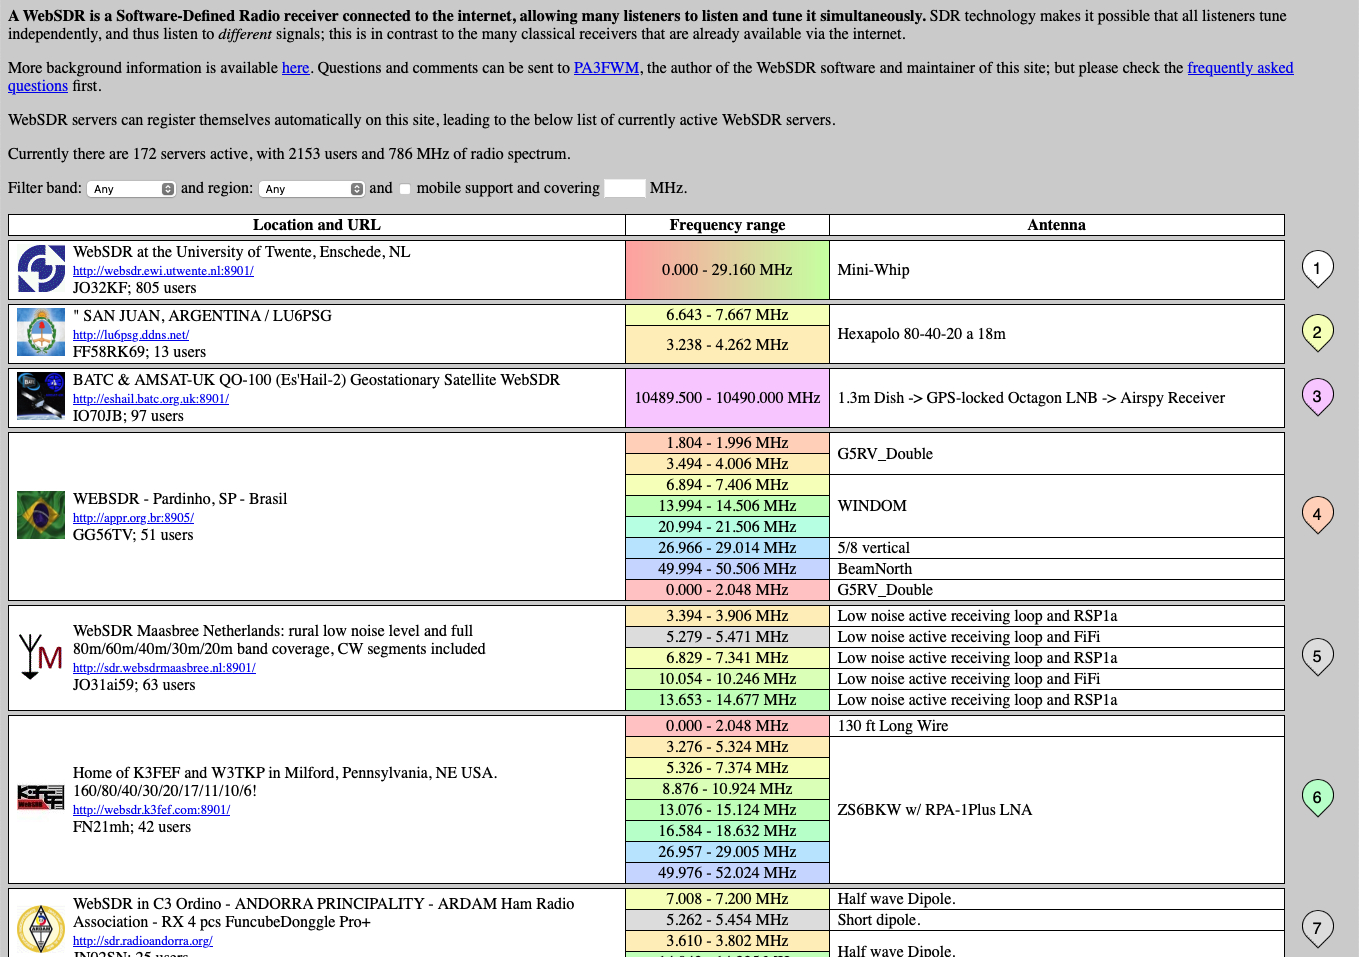
\includegraphics{include/img/websdr-org.png}

}

\caption{websdr.org}

\end{figure}

Scroll down to see all of the places around the world where there are
webSDR stations to listen to. You can pick any one you like, but we'll
focus on one in the U.S. that we use often because it's close to our
location.

\hypertarget{visit-the-k3fef-web-sdr}{%
\section*{Visit the K3FEF web SDR}\label{visit-the-k3fef-web-sdr}}
\addcontentsline{toc}{section}{Visit the K3FEF web SDR}

\markright{Visit the K3FEF web SDR}

Go to \url{http://websdr.k3fef.com}. This station is located in Milford,
Pennsylvania on the Delaware River. It's the closest one to Penn State.
So, it's often one to consult for listeners in our area.

Here is a screenshot of the K3FEF control panel.

\begin{figure}

{\centering 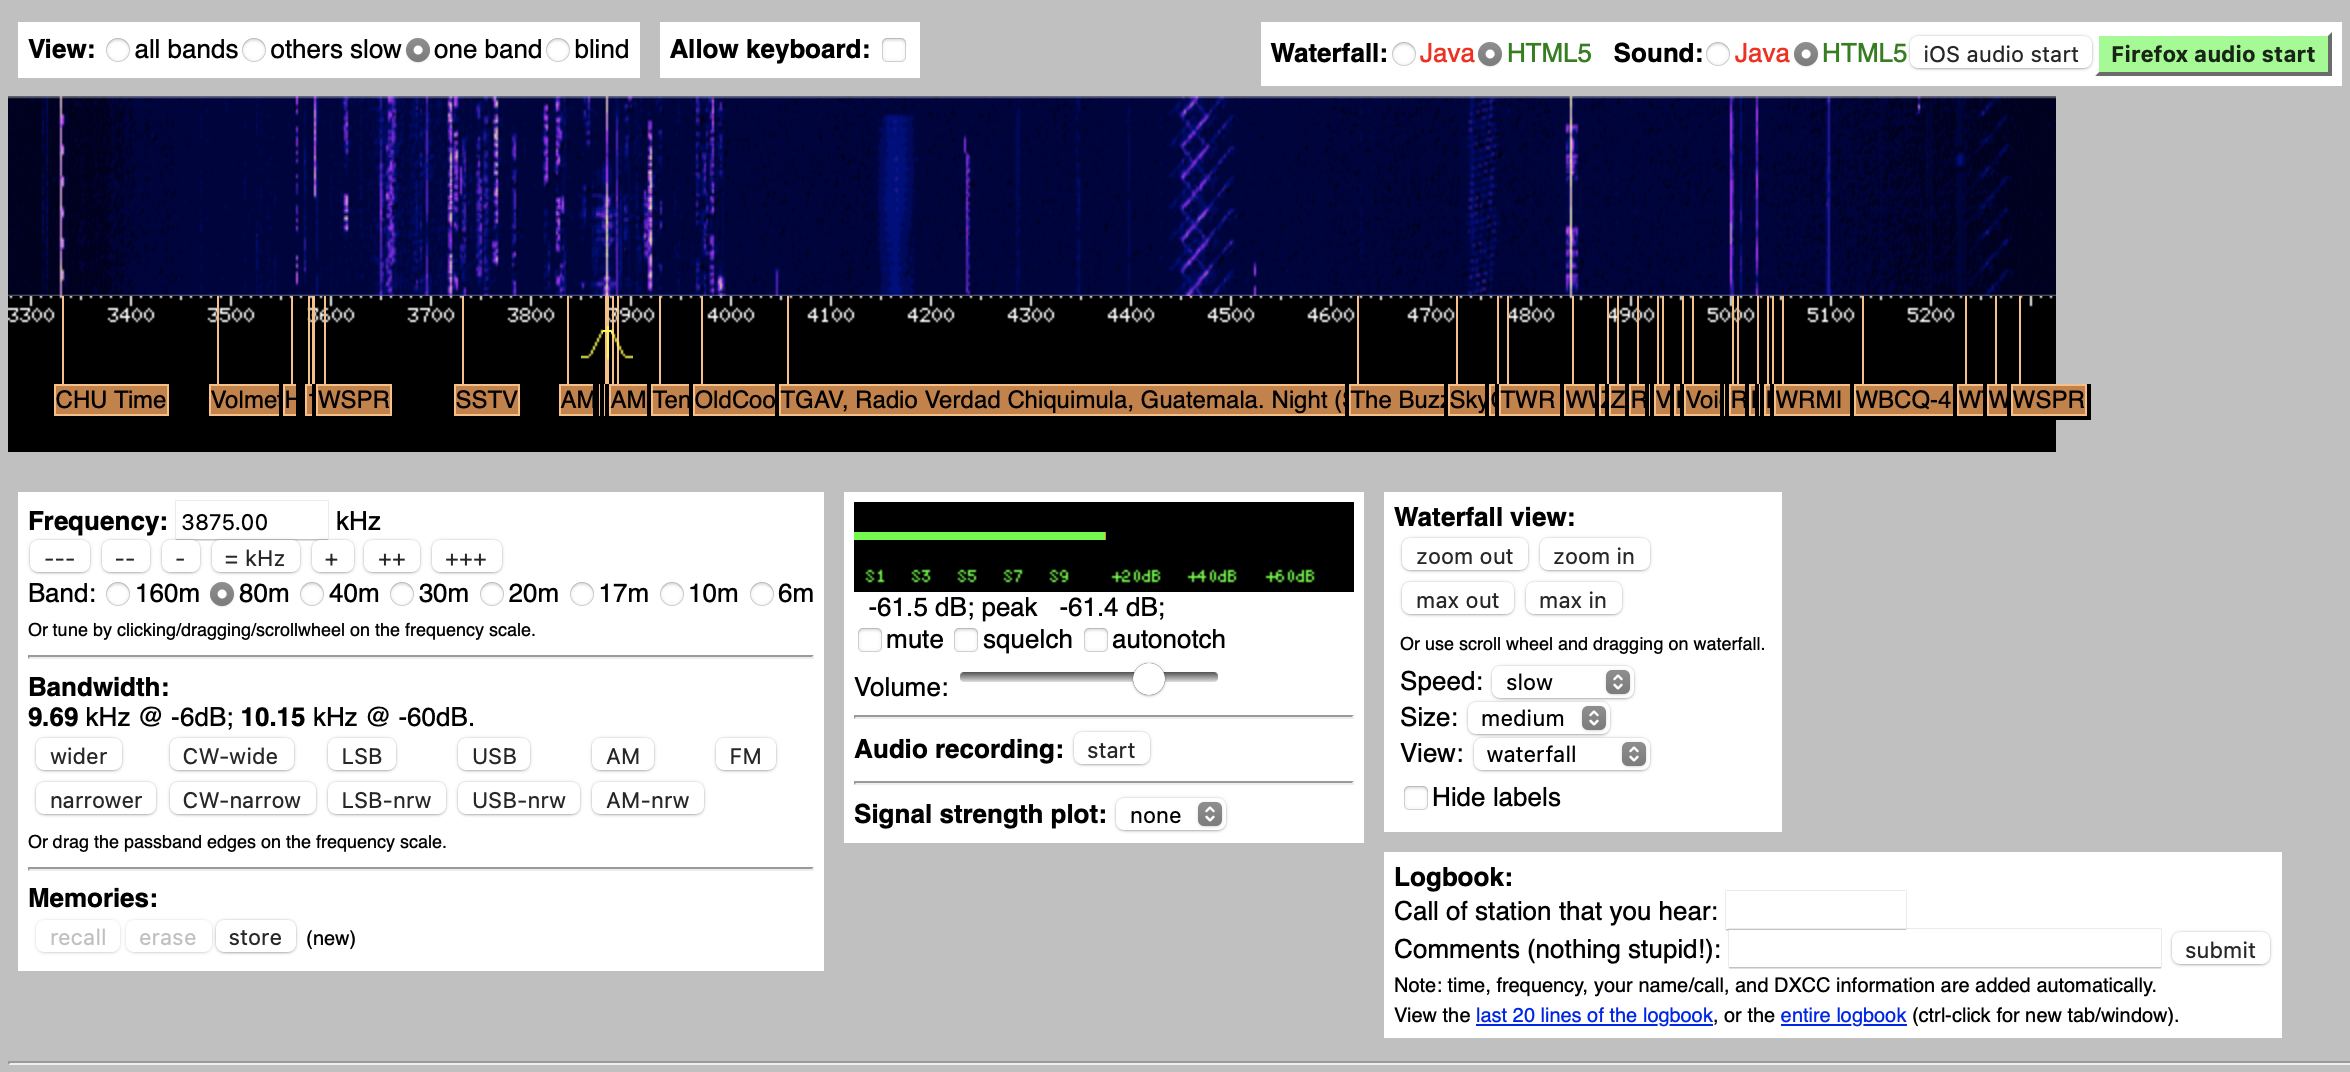
\includegraphics{include/img/k3fef-websdr.png}

}

\caption{K3FEF webSDR at http://websdr.k3fef.com}

\end{figure}

The dark blue area at the top depicts the band activity at the time you
visit. The figure shows radio signals being heard by K3FEF from about
3300 kHz (3.3 MHz) below the 80m ham band to 5300 kHz (5.5 MHz) in the
60m ham band.

If you are watching this on the web, you will see upwards motion. This
is how the webSDR depicts the time series or history of recent signals.
So, time is on the vertical axis of this two-dimensional figure.
Sometimes this type of frequency-over-time display is called a
waterfall. Except this waterfall falls upward.

Below the figure are some orange `flag' or labels that other listeners
have added. These identify the specific transmissions. If you look
especially closely, you'll also see a yellow `hump' around 3875 kHz.
That's the specific frequency this SDR defaulted to when we opened it
up. We'll explain what the yellow hump means a bit later.

In the static figure above, you'll notice a lot of activity between
about 3550 kHz and 4000 kHz. The 80m and 75m ham bands occupy 3500-4000
kHz, so those are hams communicating. The figure was taken about 8:00am
EDT (1200 UTC). These bands are usually open from evening to
mid-morning.

Let's focus on the white panel below the waterfall.

\begin{figure}

{\centering 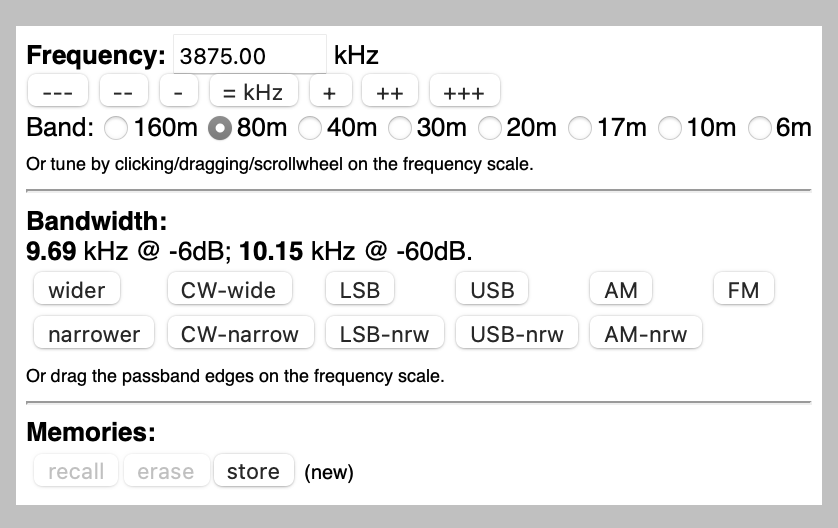
\includegraphics{include/img/k3fef-websdr-panel-1.png}

}

\caption{K3FEF webSDR at http://websdr.k3fef.com}

\end{figure}

The panel's \textbf{Frequency} control tells us that our radio is tuned
to 3875 MHz, right in the middle of the 80/75m band, the phone (voice)
portion. There are some controls to change the frequency, then below
that, a set of buttons to change the band. The highlighted button
confirms that we are in the 80/75m band\footnote{Why is it called the
  80m band and also the 75m band and sometimes the 80m/75m band? Well,
  300/3.5=\texttt{r\ 300/3.5} and 300/4.0=\texttt{r\ 300/4.0}. So, the
  approximate speed of light (in millions of meters per second) divided
  by the frequency in MHz gives us the approximate wavelength of radio
  waves. It's a single 0.5 MHz (500 kHz) chunk of frequency reserved
  exclusively for amateurs that roughly bracket \textasciitilde80-75m.}.

Notice that the K3FEF webSDR covers ham bands up through 6m. It does not
cover the 15m or 12m bands, though.

Below the \textbf{Frequency} control is a set of buttons that control
\textbf{Bandwidth}. No, bandwidth is not the size of your favorite jazz
combo. Bandwidth means how much of the frequency spectrum the webSDR is
capturing at this moment, centered on the 3875 {[}kHz{]} frequency we
just mentioned. Different types of radio transmissions (voice vs.~Morse
code/{[}CW{]} for example) have different bandwidths. We often want to
adjust our bandwidth to match the type of signal. If the bandwidth is
much wider than the signal, we're just adding noise. If the bandwidth is
much narrower than the signal, we can lose information. Voice
transmissions have wider bandwidth than Morse code/{[}CW{]}. And
different types of voice signals have different bandwidths. {[}FM{]} is
the widest, for example; {[}AM{]} is in the middle; and single sideband
{[}SSB{]} the narrowest.

Our bandwidth is 9.69 {[}kHz{]} @ -6 {[}dB{]} \footnote{This means that
  if we look at the peak signal at 3875 kHz and calculate the point on
  both sides of 3875 kHz where the signal drops by 6 decibels (db) or
  about 4-fold, we're left with 9.69 kHz of signal. The \emph{width} of
  the yellow `hump' in the waterfall display shows us this bandwidth
  visually.}. That's wide, except for broadcast FM stations. We can
adjust the bandwidth incrementally using the
\emph{wider}/\emph{narrower} buttons or adjust the bandwidth to match a
specific type of signal: \emph{CW-wide}/\emph{CW-nrw} (narrow),
\emph{LSB-wide}/\emph{LSB-nrw}, \emph{USB-wide}/\emph{USB-nrw},
\emph{AM-wide}/\emph{AM-nrw}, and \emph{FM}. We can also adjust the
bandwidth manually.

\hypertarget{find-a-signal-to-listen-to}{%
\section*{Find a signal to listen to}\label{find-a-signal-to-listen-to}}
\addcontentsline{toc}{section}{Find a signal to listen to}

\markright{Find a signal to listen to}

Click on the {green} \emph{Firefox audio start} button in the upper
right hand of the screen. Be ready to adjust the volume on your computer
downward! Or adjust the volume in the panel or even mute it (see the
figure below).

Chances are that you'll just hear static since we're on a random
frequency.

\begin{figure}

{\centering 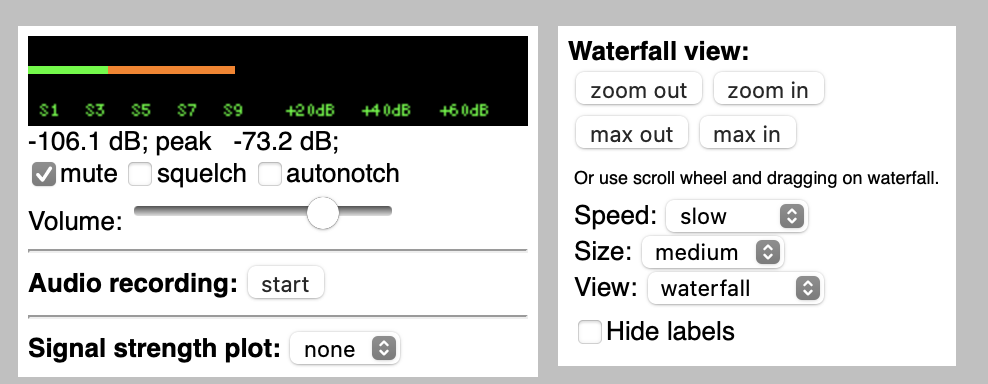
\includegraphics{include/img/k3fef-websdr-panel-2.png}

}

\caption{K3FEF webSDR at http://websdr.k3fef.com}

\end{figure}

To fix that, look at the \textbf{Waterfall view} panel. Zoom \emph{in}
by clicking on the button a couple of times. Sometimes zooming moves
window beyond the frequency where you are currently tuned. If that
happens, you won't see the yellow `hump' anymore.

But you can find it again by clicking on the blue/purple area in the
waterfall and dragging to the left or the right to put your current
frequency--3875 kHz for our example--in the middle of the panel.

In our case, there's a very strong signal around 3810 kHz.

\begin{figure}

{\centering 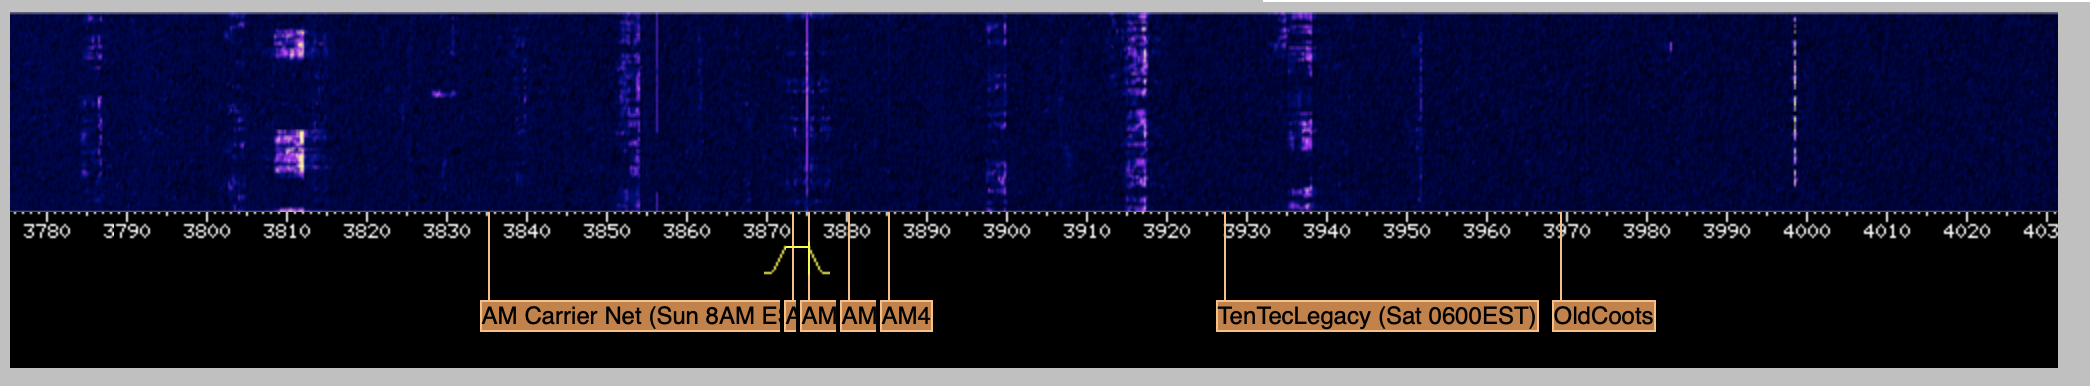
\includegraphics{include/img/k3fef-websdr-3875.png}

}

\caption{K3FEF webSDR at http://websdr.k3fef.com}

\end{figure}

Notice that most of the signal around 3810 kHz (3.810 MHz) lies
\emph{below} 3810. That's because on 75m and 80m, hams use Lower
Sideband ({[}LSB{]}) for {[}phone{]} transmissions. To see another
example of what LSB and upper sideband ({[}USB{]}) signals look like,
see \protect\hyperlink{fig:hf-signals}{figure below}.

\hypertarget{going-further}{%
\section*{Going further}\label{going-further}}
\addcontentsline{toc}{section}{Going further}

\markright{Going further}

Now that you've gotten familiar with the K3FEF WebSDR, you might be
curious to know what else there is to listen to, and equally important,
\emph{when}. I say when because the high frequency (HF) bands change
their propagation characteristics--how far and how well they convey
radio signals--based on the time of day, season of the year, and phase
of the 11-year sunspot cycle, among other characteristics. We'll do a
deeper dive on these topics in the \href{}{Band Conditions} quest. For
now, here are some general rules of thumb about \emph{where} to listen
and \emph{when}:

75m/80m: These bands provide long distance (DX) communication at night,
especially in the winter months, and regional communication in the early
morning hours.

40m: This band also provides long distance communication at night and
more reliable regional communication in the daylight hours.

20m: This band supports long distance communication during daylight
hours.

17m: This band supports long distance communication during daylight
hours.

15m: This band supports long distance communication during daylight
hours.

12m: This band supports long distance communication during daylight
hours during the peak times of the sunspot cycle. It is often closed at
the depth of that cycle.

10m: This band supports long distance communication during daylight
hours during the peak times of the sunspot cycle. It is often closed at
the depth of that cycle.

Now, you might be interested to know what's worth listening to or for.
My recommendation would be for you to listen to established nets that
have published schedules. For example, you can search for a net that
meets specific criteria on the ARRL website at
\href{http://www.arrl.org/arrl-net-directory-search}{www.arrl.org/arrl-net-directory-search}.
You may also want to try the \href{https://netfinder.radio}{NetFinder}
site.

\begin{tcolorbox}[enhanced jigsaw, colframe=quarto-callout-note-color-frame, opacitybacktitle=0.6, colback=white, arc=.35mm, toprule=.15mm, bottomtitle=1mm, breakable, titlerule=0mm, toptitle=1mm, title=\textcolor{quarto-callout-note-color}{\faInfo}\hspace{0.5em}{Note}, rightrule=.15mm, coltitle=black, left=2mm, colbacktitle=quarto-callout-note-color!10!white, opacityback=0, bottomrule=.15mm, leftrule=.75mm]

It would be good to add some information about some SWL stations that
are easy to hear.

Also, there are some nets that are good examples, e.g., the M-Su Rooster
Net on 3.990 MHz and the YSL System Nets, and some frequencies that are
\emph{not} good examples, e.g., 7.200 MHz and 14.313 MHz.

\end{tcolorbox}

\hypertarget{quest-dmr}{%
\chapter*{Quest: DMR}\label{quest-dmr}}
\addcontentsline{toc}{chapter}{Quest: DMR}

\markboth{Quest: DMR}{Quest: DMR}

\begin{tcolorbox}[enhanced jigsaw, colframe=quarto-callout-tip-color-frame, opacitybacktitle=0.6, colback=white, arc=.35mm, toprule=.15mm, bottomtitle=1mm, breakable, titlerule=0mm, toptitle=1mm, title=\textcolor{quarto-callout-tip-color}{\faLightbulb}\hspace{0.5em}{Tip}, rightrule=.15mm, coltitle=black, left=2mm, colbacktitle=quarto-callout-tip-color!10!white, opacityback=0, bottomrule=.15mm, leftrule=.75mm]

These activities are relevant to the following Technician license pool
questions:

\protect\hyperlink{T2B12}{T2B12}; \protect\hyperlink{T4B07}{T4B07};
\protect\hyperlink{T8D02}{T8D02}; \protect\hyperlink{T8D07}{T8D07}.

\end{tcolorbox}

You can listen to Digital Mobile Radio ({[}DMR{]}) transmissions across
the globe on the web without having to log in or have a ham radio
license.

In this quest, we'll listen in on some conversations using DMR.

Remember, as a ham, all of our communications except those controlling
aircraft or satellites are presumed public.

\hypertarget{visit-the-brandmeister-network}{%
\section*{\texorpdfstring{Visit the
\href{https://brandmeister.network}{Brandmeister
Network}}{Visit the Brandmeister Network}}\label{visit-the-brandmeister-network}}
\addcontentsline{toc}{section}{Visit the
\href{https://brandmeister.network}{Brandmeister Network}}

\markright{Visit the Brandmeister Network}

The Brandmeister Network is one of the largest organizations providing
DMR services. The Brandmeister Network maintains a
\href{https://hose.brandmeister.network}{hoseline site} that shows all
of the DMR traffic going through the Network.

You will see something like the following:

\begin{figure}

{\centering 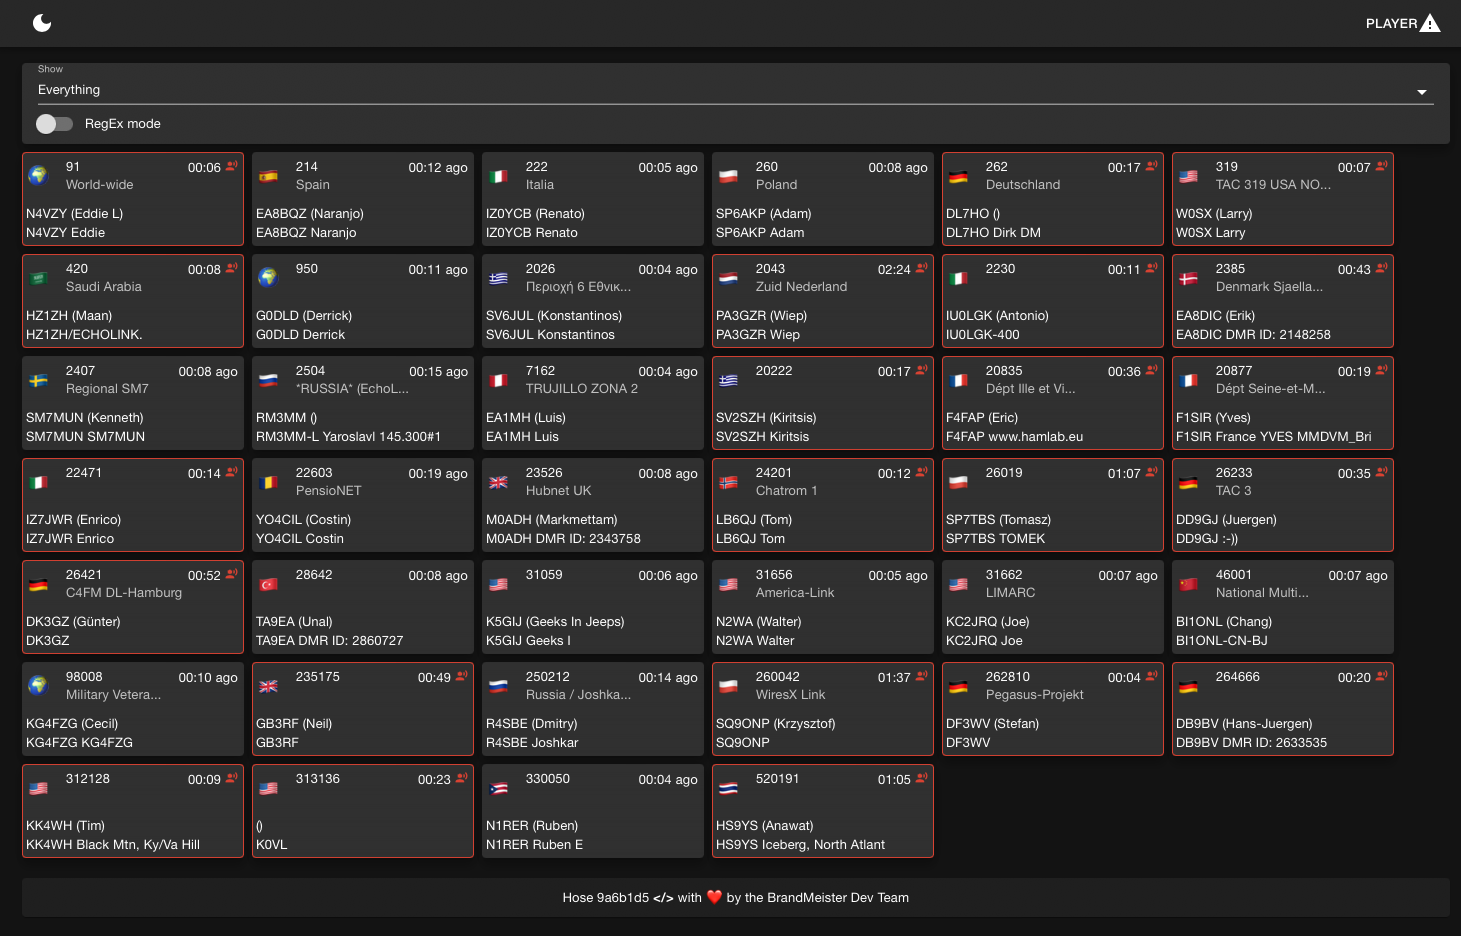
\includegraphics[width=1\textwidth,height=\textheight]{include/img/brandmeister-hoseline-2023-04-03.png}

}

\caption{Brandmeister DMR hoseline as of 2023-04-03 about 1745Z}

\end{figure}

This shows all of the stations connected to the Brandmeister network in
the entire world.

\hypertarget{click-on-an-active-qso}{%
\section*{Click on an active QSO}\label{click-on-an-active-qso}}
\addcontentsline{toc}{section}{Click on an active QSO}

\markright{Click on an active QSO}

To listen in on one of these {[}QSO{]}s, click on an active QSO. Active
QSOs will be outlined in {red}.

\begin{figure}

{\centering 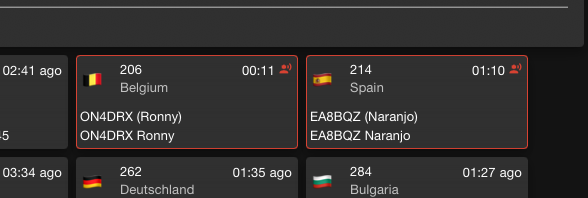
\includegraphics{include/img/brandmeister-network-active-qso.png}

}

\end{figure}

You can also listen in on specific talkgroups. A talkgroup is like a
repeater, except that it repeats signals from stations connected via the
internet. There is often traffic on talkgroup 91 (Worldwide) or
talkgroup 93 (North America), so let's listen in on those.

Click the PLAYER button in the upper right hand corner.

This will open a small panel where you can select what talkgroups to
listen to or which stations to monitor.

\begin{figure}

{\centering 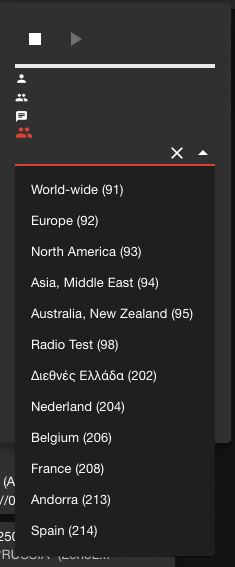
\includegraphics{include/img/brandmeister-hoseline-player-panel.png}

}

\caption{PLAYER panel from hose.brandmeister.network}

\end{figure}

\hypertarget{quest-aprs}{%
\chapter*{Quest: APRS}\label{quest-aprs}}
\addcontentsline{toc}{chapter}{Quest: APRS}

\markboth{Quest: APRS}{Quest: APRS}

In this quest, we'll check-in on the Automatic Packet Reporting System
(APRS) where hams across the world provide real-time information about
their locations and exchange messages, including weather reports.

\hypertarget{visit-aprs.fi}{%
\section*{\texorpdfstring{Visit
\href{https://aprs.fi}{APRS.fi}}{Visit APRS.fi}}\label{visit-aprs.fi}}
\addcontentsline{toc}{section}{Visit \href{https://aprs.fi}{APRS.fi}}

\markright{Visit APRS.fi}

The first time you visit this site, it may show you a view of APRS
activity near the APRS.fi website author's home in Finland (hence the
.fi web domain).

Feel free to scroll out using the minus (-) button in the lower right
hand corner and then click and drag to another location. For example,
here is a view near Philadelphia, PA.

\begin{figure}

{\centering 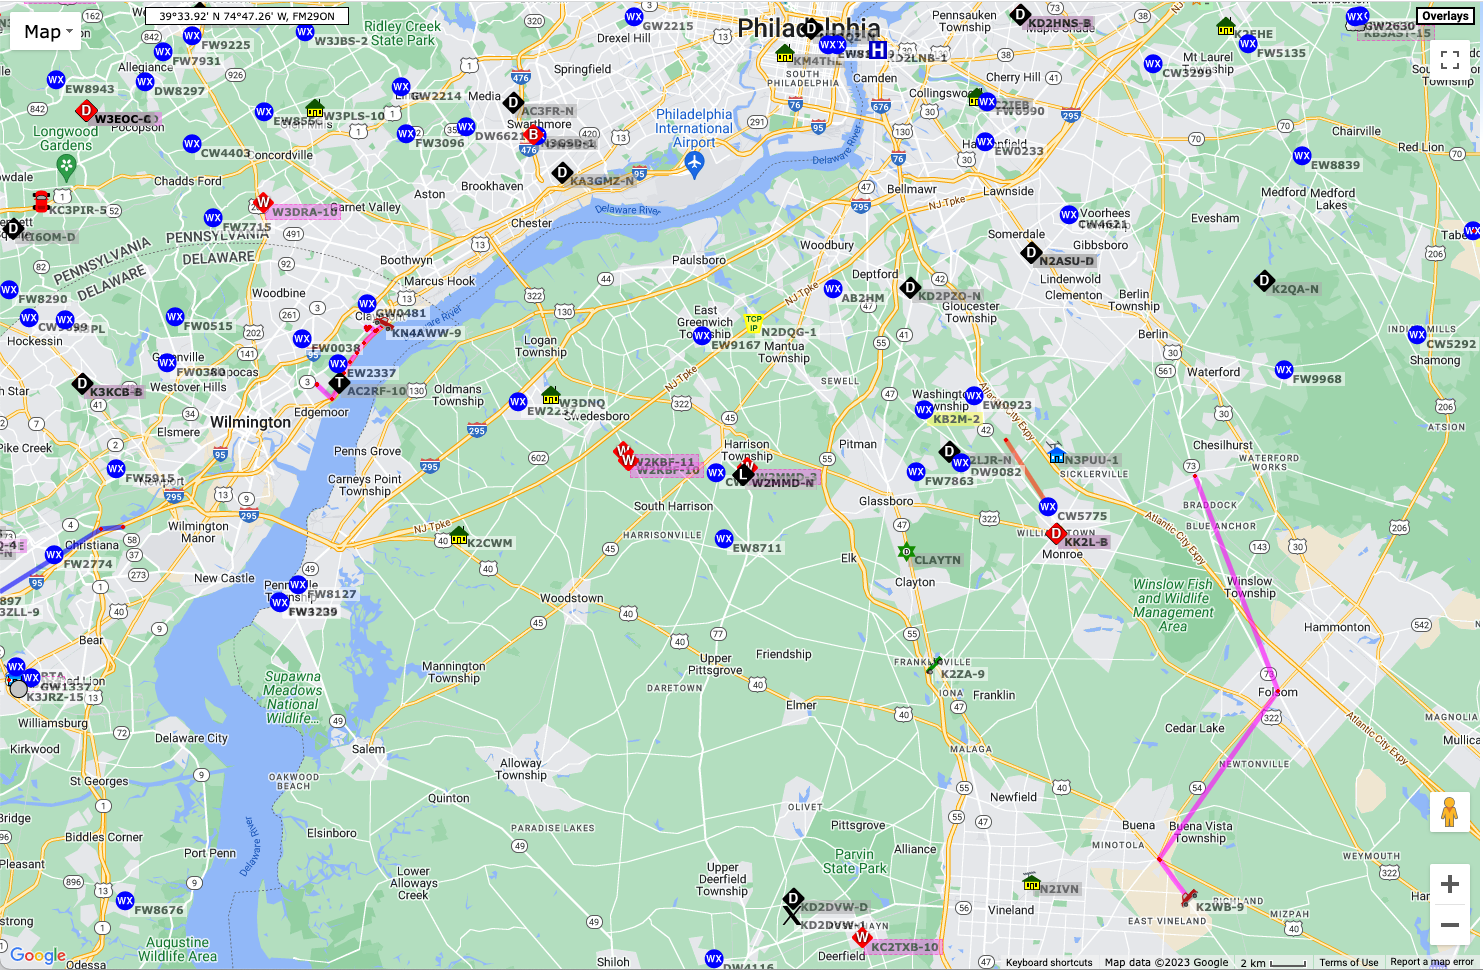
\includegraphics[width=1\textwidth,height=\textheight]{include/img/aprs.fi-2023-04-05.png}

}

\caption{APRS activity near Philadelphia, PA on 2023-04-05}

\end{figure}

Notice that some of the symbols look like vehicles and have a track that
appears to show where they've been.

\hypertarget{get-more-info}{%
\section*{Get more info}\label{get-more-info}}
\addcontentsline{toc}{section}{Get more info}

\markright{Get more info}

Mouse over one of those symbols.

You should see a set of lines connecting the vehicle symbol to another
one on the map. The lines show where the RF signal from the vehicle
traveled before being heard and sent over the Internet to the APRS.fi
site.

\begin{figure}

{\centering 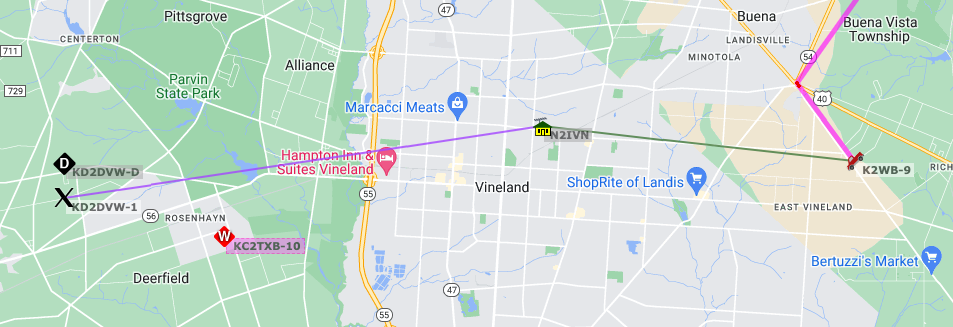
\includegraphics[width=1\textwidth,height=\textheight]{include/img/aprs-track.png}

}

\caption{APRS track of moving vehicle K2WB-9.}

\end{figure}

The figure shows the station K2WB connecting to a home-based relay
station N2IVN and the relayed signal from N2IVN being heard by KD2DVW-1.

\hypertarget{click-on-a-mobile-moving-station}{%
\section*{Click on a mobile (moving)
station}\label{click-on-a-mobile-moving-station}}
\addcontentsline{toc}{section}{Click on a mobile (moving) station}

\markright{Click on a mobile (moving) station}

Click on a mobile (moving) station's icon.

A small window will open with information about that station.

\begin{figure}

{\centering 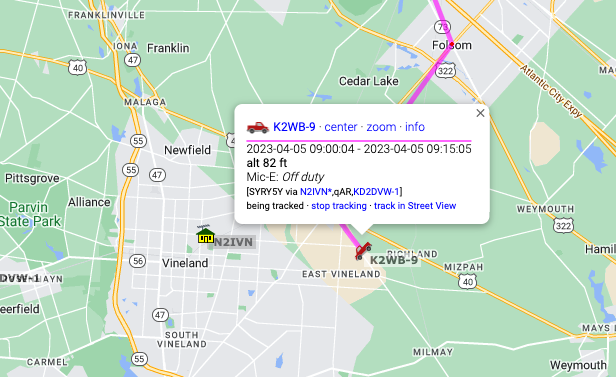
\includegraphics{include/img/aprs-k2wb-9.png}

}

\end{figure}

Click on the info button in the small window.

\begin{figure}

{\centering 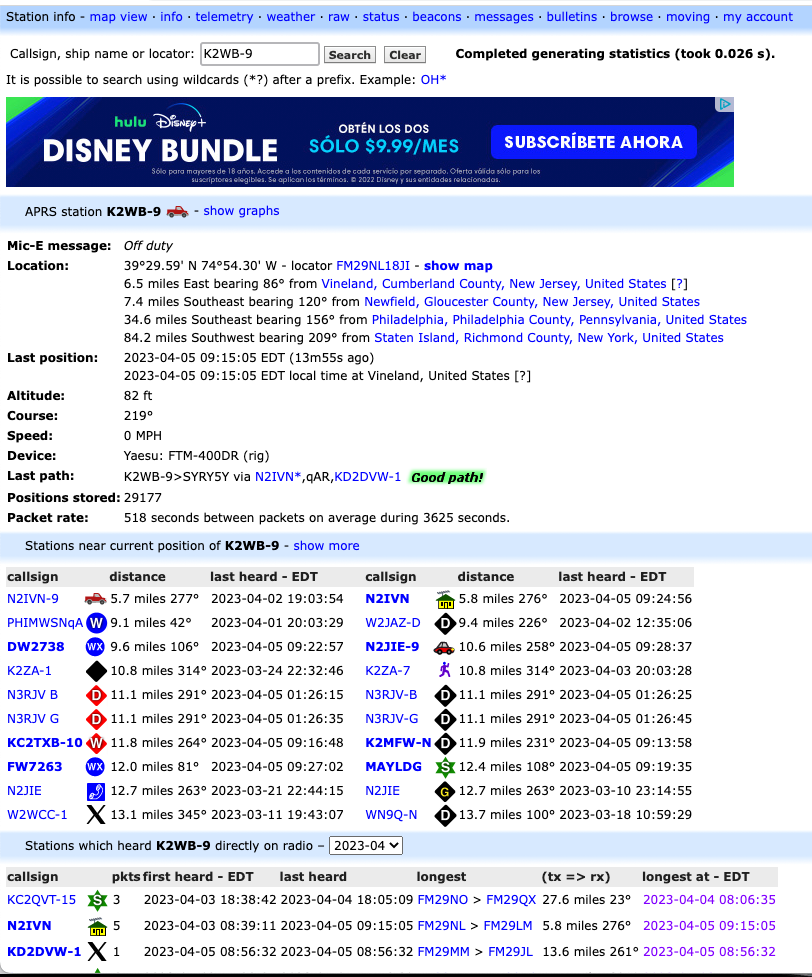
\includegraphics{include/img/aprs-k2wb-9-info.png}

}

\end{figure}

\hypertarget{find-the-international-space-station-iss}{%
\section*{Find the International Space Station
(ISS)}\label{find-the-international-space-station-iss}}
\addcontentsline{toc}{section}{Find the International Space Station
(ISS)}

\markright{Find the International Space Station (ISS)}

The International Space Station has an APRS beacon! So, if you have an
APRS-enabled radio set up you can hear the ISS when it passes near your
location (and you are listening on the ISS APRS frequency of 144.825 MHz
in the 2m band).

Enter \texttt{ISS} in the ``Track callsign:'' window in the upper right
of the aprs.fi site.

I did this on the morning of 2023-04-05, and here was the result.

\begin{Shaded}
\begin{Highlighting}[]
\NormalTok{knitr}\SpecialCharTok{::}\FunctionTok{include\_graphics}\NormalTok{(}\StringTok{"include/img/aprs{-}iss{-}2023{-}04{-}05.png"}\NormalTok{)}
\end{Highlighting}
\end{Shaded}

\begin{figure}[H]

{\centering 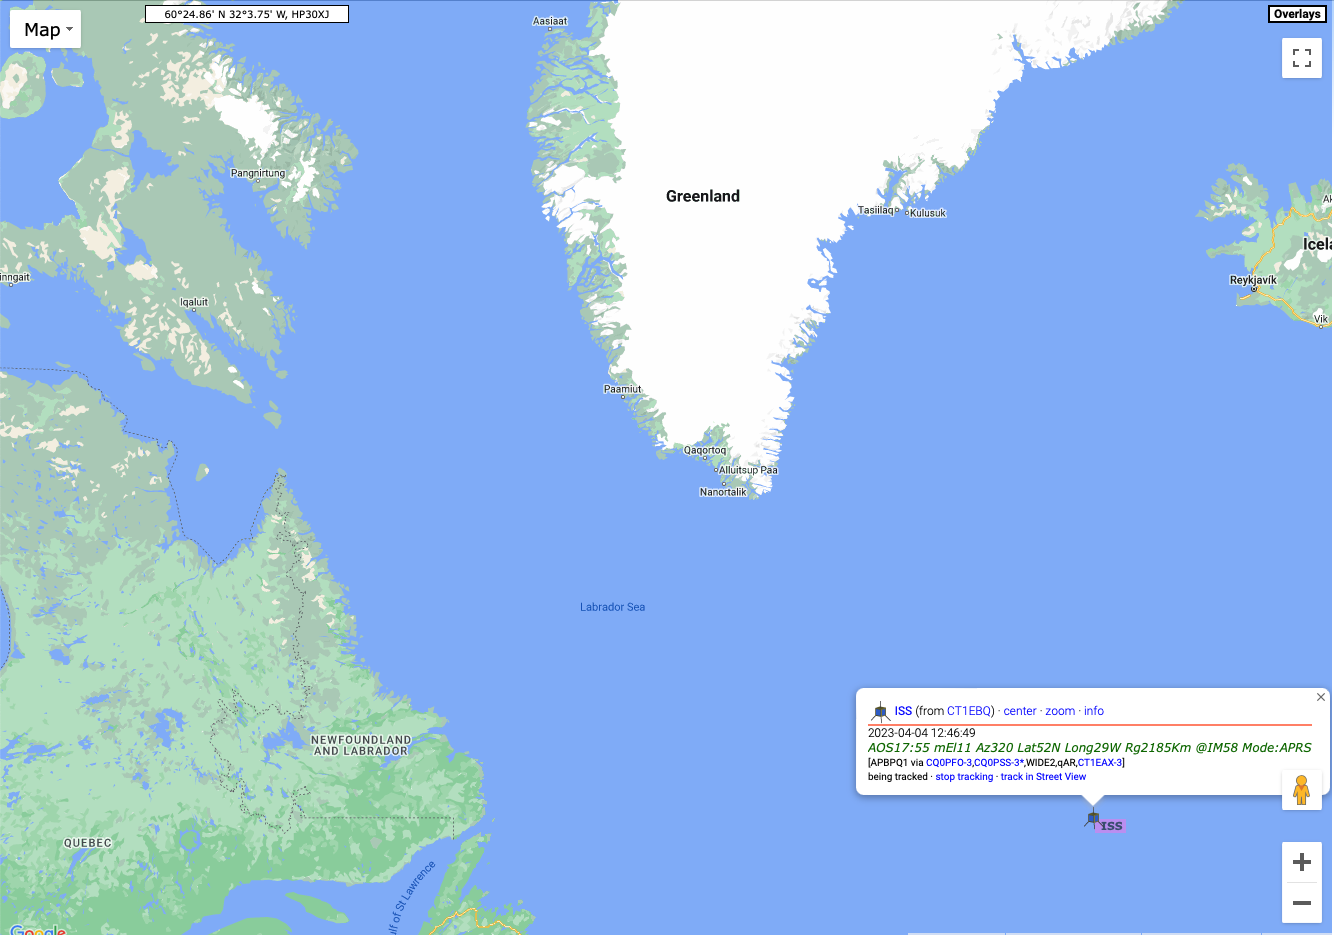
\includegraphics{include/img/aprs-iss-2023-04-05.png}

}

\end{figure}

The ISS was somewhere over the North Atlantic Ocean. I say \emph{was},
because if you look closely, you'll see that the last time the ISS was
heard on APRS was on 2023-04-04, about 20 hours before the time I took
this screenshot. The APRS beacon goes on and off from time to time.

\hypertarget{quest-sattelites}{%
\chapter*{Quest: Satellite tracking}\label{quest-sattelites}}
\addcontentsline{toc}{chapter}{Quest: Satellite tracking}

\markboth{Quest: Satellite tracking}{Quest: Satellite tracking}

Hams have launched satellites that permit communication across large
areas, and the International Space Station (ISS) has ham radio equipment
on board.

\hypertarget{visit-httpswww.n2yo.comspace-station}{%
\section*{\texorpdfstring{Visit
\url{https://www.n2yo.com/space-station/}}{Visit https://www.n2yo.com/space-station/}}\label{visit-httpswww.n2yo.comspace-station}}
\addcontentsline{toc}{section}{Visit
\url{https://www.n2yo.com/space-station/}}

\markright{Visit https://www.n2yo.com/space-station/}

The window in the upper left will show a map of the current location of
the ISS.

The window in the upper right will show the current live video feed from
the ISS. If it's dark, that's probably because the ISS is on the night
side of the Earth.

\hypertarget{visit-the-amateur-satellite-corporation-amsat}{%
\section*{\texorpdfstring{Visit the
\href{https://www.amsat.org/}{Amateur Satellite Corporation
(AMSAT)}}{Visit the Amateur Satellite Corporation (AMSAT)}}\label{visit-the-amateur-satellite-corporation-amsat}}
\addcontentsline{toc}{section}{Visit the
\href{https://www.amsat.org/}{Amateur Satellite Corporation (AMSAT)}}

\markright{Visit the Amateur Satellite Corporation (AMSAT)}

The \href{https://www.amsat.org/}{Amateur Satellite Corporation (AMSAT)}
also maintains a tracking \href{https://www.amsat.org/track/}{site.}

Here you can choose to track a number of amateur satellites.

\begin{figure}

{\centering 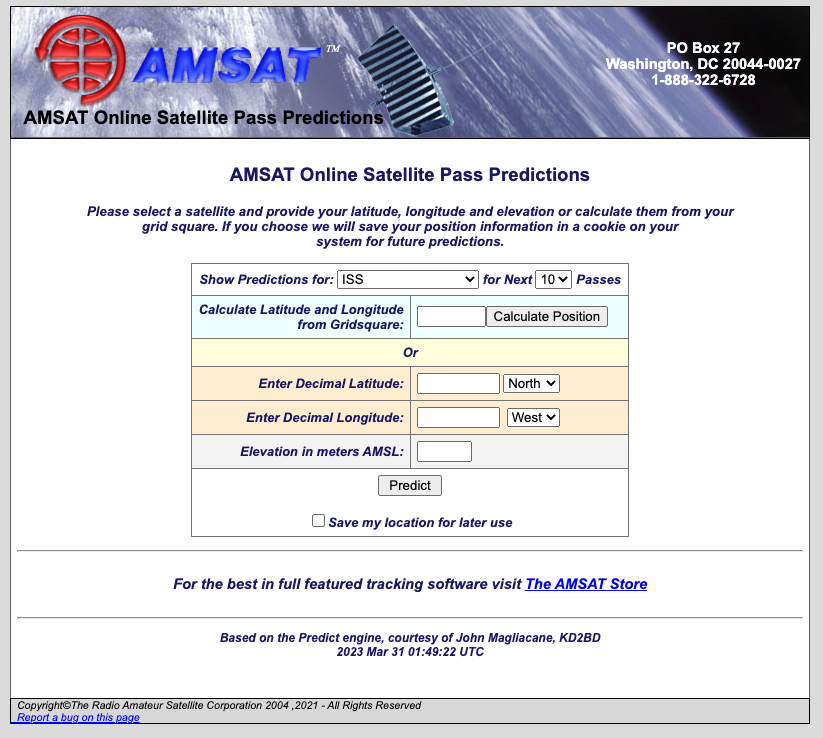
\includegraphics{include/img/amsat-track.png}

}

\end{figure}

The site will calculate the next time a satellite will pass over your
location. You need to give it your latitude and longitude or your grid
square for this to work.

What's a grid square? Well every part of the Earth has been assigned a
code that is a combination of letters and numbers. The codes are part of
the
\href{https://en.wikipedia.org/wiki/Maidenhead_Locator_System}{Maidenhead
Locator System}.

By \textless a href=``https://en.wikipedia.org/wiki/User:Mysid''
class=``extiw''
title=``w:User:Mysid''\textgreater Mysid\textless/a\textgreater{} -
Self-drawn in Inkscape., Public Domain, Link

See the following two figures from Wikipedia.

By User:Denelson83 - \textless a rel=``nofollow'' class=``external
free''
href=``http://visibleearth.nasa.gov/view\_rec.php?id=2433''\textgreater http://visibleearth.nasa.gov/view\_rec.php?id=2433\textless/a\textgreater,
Public Domain, Link

By Oona Räisänen (\textless a
href=``https://en.wikipedia.org/wiki/User:Mysid'' class=``extiw''
title=``w:User:Mysid''\textgreater Mysid\textless/a\textgreater) - Base
map from \textless a
href=``//commons.wikimedia.org/wiki/File:Blank\_map\_of\_Europe\_(polar\_stereographic\_projection)\_cropped.svg''
class=``mw-redirect'' title=``File:Blank map of Europe (polar
stereographic projection) cropped.svg''\textgreater Image:Blank map of
Europe (polar stereographic projection)
cropped.svg\textless/a\textgreater; Grid drawn in Inkscape and based on
the (public domain) output of Great Circle Maps v2.3., CC BY-SA 3.0,
Link

To find out your particular grid square, visit
\url{https://www.karhukoti.com/maidenhead-grid-square-locator}. The site
gives you both your latitude and longitude and grid square. The figure
below shows my approximate location and grid square, FN10.

\begin{figure}

{\centering 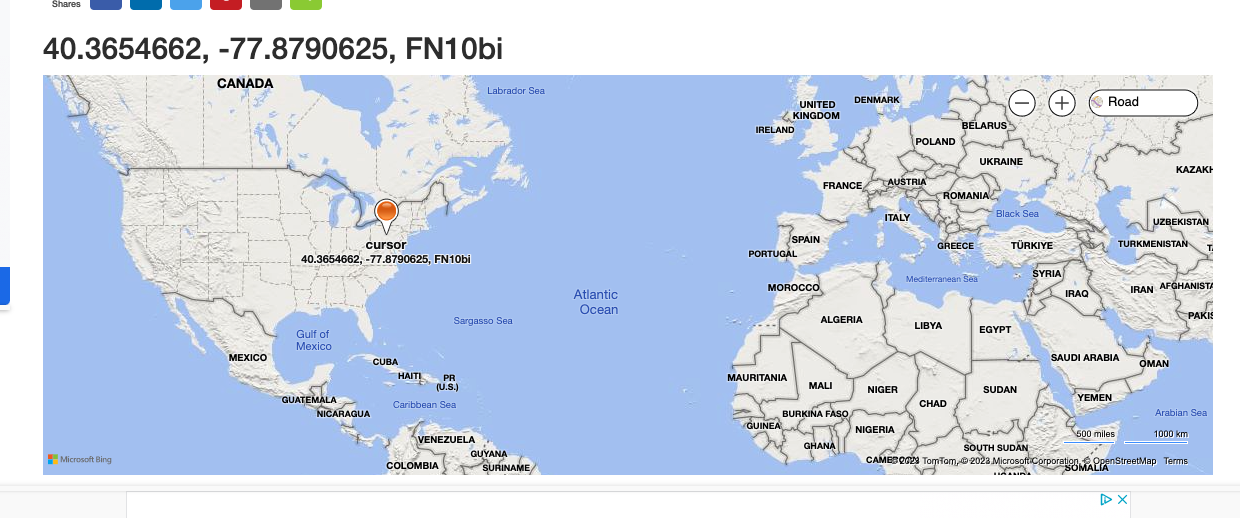
\includegraphics{include/img/karhukoti-grid-square.png}

}

\end{figure}

Notice that grid squares can be increasingly precise. For our purposes
now, the four character grid square is sufficient. Hams who operate
digital modes like FT8 and FT4 using the WSJT-X software use grid
squares, too. And some hams ``collect'' contacts in different grid
squares. For now, we'll use our grid square to calculate when the ISS
will pass over our grid square.

\hypertarget{when-will-the-iss-pass-over-you-next}{%
\section*{When will the ISS pass over you
next?}\label{when-will-the-iss-pass-over-you-next}}
\addcontentsline{toc}{section}{When will the ISS pass over you next?}

\markright{When will the ISS pass over you next?}

Enter your grid square in the AMSAT Tracking site.

Hit ``Calculate Position'' to let the site calculate your latitude and
longitude, then hit the ``Predict'' button.

The results show the next several passes of the {[}ISS{]} over my grid
square. Yours will be different, even if you live in my grid square,
because the ISS is always moving.

\begin{figure}

{\centering 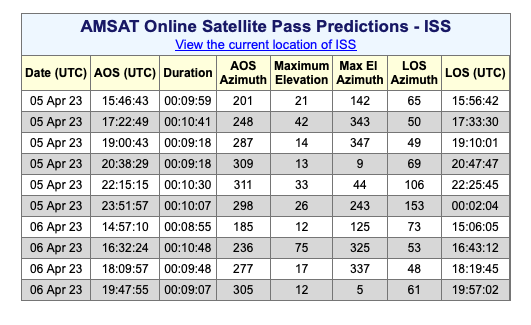
\includegraphics{include/img/amsat-iss-pred-fn10.png}

}

\end{figure}

\hypertarget{quest_pota}{%
\chapter*{Quest: POTA/SOTA hunting}\label{quest_pota}}
\addcontentsline{toc}{chapter}{Quest: POTA/SOTA hunting}

\markboth{Quest: POTA/SOTA hunting}{Quest: POTA/SOTA hunting}

\hypertarget{about-1}{%
\section*{About}\label{about-1}}
\addcontentsline{toc}{section}{About}

\markright{About}

In this quest, you will ``hunt'' hams who are operating using portable
stations from one of several thousand parks around the world as part of
the Parks on the Air (POTA) system.

\hypertarget{visit-pota.app}{%
\section*{Visit Pota.app}\label{visit-pota.app}}
\addcontentsline{toc}{section}{Visit Pota.app}

\markright{Visit Pota.app}

The site shows hams who are active on the air \emph{right now} and on
what frequencies and using which modes.

\hypertarget{choose-a-station-to-hunt}{%
\section*{Choose a station to ``hunt''}\label{choose-a-station-to-hunt}}
\addcontentsline{toc}{section}{Choose a station to ``hunt''}

\markright{Choose a station to ``hunt''}

By hunt, of course, we mean try to hear on the radio. Once you're
licensed with appropriate privileges, you can try to make contact. For
now, let's just try to hear the station.

You have some decisions to make. Which mode, CW, FT8, or phone? Which
band?

Unless you have already set up a receiver to copy and decode FT8, you
can eliminate stations using {[}FT8{]} or {[}FT4{]}. Phone is the
easiest, but also requires the best band conditions.

Here are some rules of thumb to guide your choices:

\begin{enumerate}
\def\labelenumi{\arabic{enumi}.}
\item
  The lower frequency (higher wavelength) bands (160m, 80m/75m, 60m, and
  40m) propagate longer distances at night than during the day. During
  the early morning hours, 80m/75m might support regional propagation,
  meaning you can hear stations within several hundred miles of your
  location. 60m and 40m might also work for regional communication
  throughout the day.
\item
  The higher bands (30m, 20m, 17m, 15m, 12m, and 10m) are long distance
  (DX) bands and are most active during the day and under good solar
  conditions.
\end{enumerate}

Once you've chosen a station to hunt, you can try to hear them on a
WebSDR.

\hypertarget{open-websdr}{%
\section*{Open WebSDR}\label{open-websdr}}
\addcontentsline{toc}{section}{Open WebSDR}

\markright{Open WebSDR}

If you pick a WebSDR near your location, then you'll need to consider
the rules of thumb above.

If you pick a WebSDR somewhere else, you'll have to think like a ham in
one of those locations: What bands are open to hams and to what parts of
the world from that location?

\hypertarget{tune-to-the-pota-station-frequency}{%
\section*{Tune to the POTA station
frequency}\label{tune-to-the-pota-station-frequency}}
\addcontentsline{toc}{section}{Tune to the POTA station frequency}

\markright{Tune to the POTA station frequency}

If the station is still active on the frequency and propagation to the
WebSDR location is good, you should see a signal in the waterfall. Try
to copy the station? Can you hear the callsign? Can you hear any
stations trying to call.

\hypertarget{quest-identify-the-signal}{%
\chapter*{Quest: Identify the signal}\label{quest-identify-the-signal}}
\addcontentsline{toc}{chapter}{Quest: Identify the signal}

\markboth{Quest: Identify the signal}{Quest: Identify the signal}

\hypertarget{about-2}{%
\section*{About}\label{about-2}}
\addcontentsline{toc}{section}{About}

\markright{About}

In this quest, you'll use WebSDR or an SDR receiver to try to find and
identify various signals found on the HF and VHF/UHF bands.

\begin{figure}

{\centering 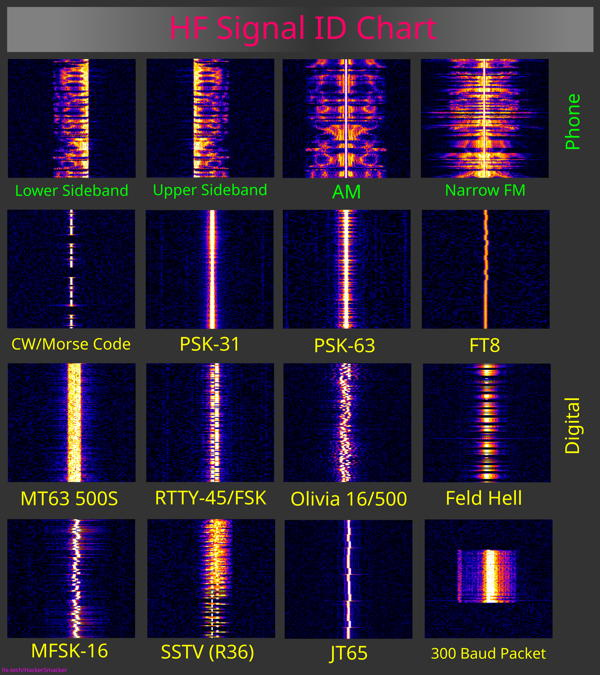
\includegraphics{include/img/hf-signal-chart-scaled.jpg}

}

\caption{HF signal chart from
https://www.reddit.com/r/amateurradio/comments/12ota0q/hf\_signal\_identification\_chart\_the\_shortawaited/?utm\_source=share\&utm\_medium=ios\_app\&utm\_name=ioscss\&utm\_content=1\&utm\_term=10}

\end{figure}

\begin{figure}

{\centering 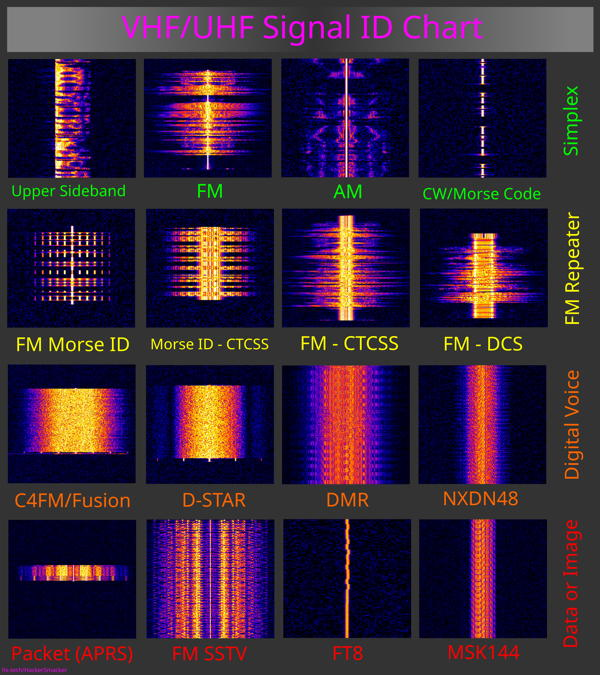
\includegraphics{include/img/vhf-signal-chart-scaled.jpg}

}

\caption{VHF signal chart from
https://www.reddit.com/r/amateurradio/comments/12okhb4/i\_whipped\_up\_a\_quick\_vhfuhf\_signal\_id\_chart\_might/?utm\_source=share\&utm\_medium=ios\_app\&utm\_name=ioscss\&utm\_content=1\&utm\_term=10}

\end{figure}

\hypertarget{quest-find-hams-in-your-area}{%
\chapter*{Quest: Find hams in your
area}\label{quest-find-hams-in-your-area}}
\addcontentsline{toc}{chapter}{Quest: Find hams in your area}

\markboth{Quest: Find hams in your area}{Quest: Find hams in your area}

\hypertarget{about-3}{%
\section*{About}\label{about-3}}
\addcontentsline{toc}{section}{About}

\markright{About}

The FCC amateur radio license database is public. That's why some hams
prefer to use a post office (P.O.) box as their permanent surface
mailing address for their license. However, the fact that the database
is public makes it easy to find hams in your geographic area.

\hypertarget{open-the-amateur-radio-license-map-application}{%
\subsection*{Open the Amateur Radio License Map
application}\label{open-the-amateur-radio-license-map-application}}
\addcontentsline{toc}{subsection}{Open the Amateur Radio License Map
application}

Visit \url{https://haminfo.tetranz.com/map}

\begin{figure}

{\centering 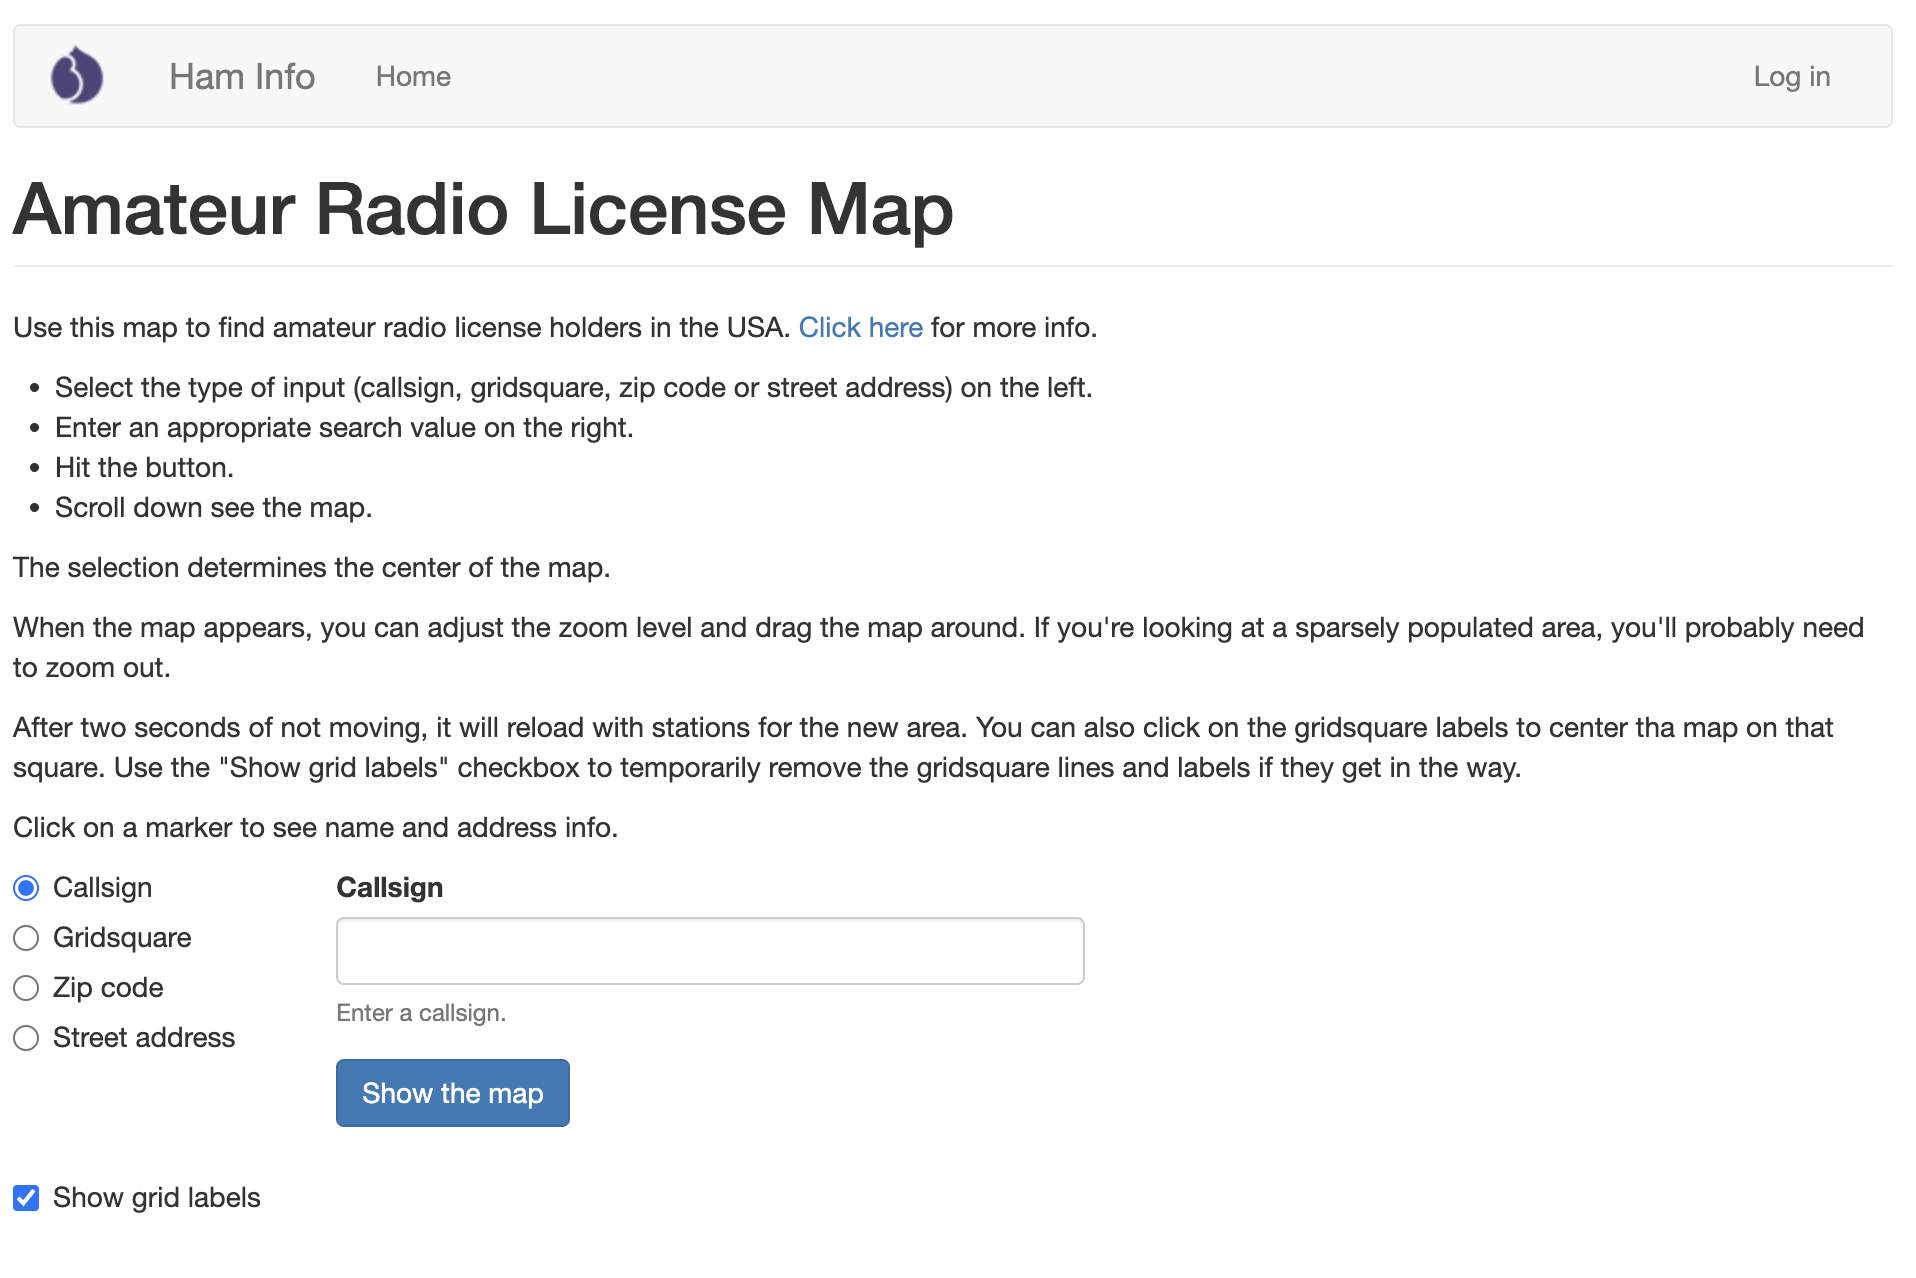
\includegraphics[width=1\textwidth,height=\textheight]{include/img/ham-radio-license-map.png}

}

\caption{https://haminfo.tetranz.com/map}

\end{figure}

\hypertarget{search-for-hams-in-your-current-zip-code}{%
\subsection*{Search for hams in your current Zip
code}\label{search-for-hams-in-your-current-zip-code}}
\addcontentsline{toc}{subsection}{Search for hams in your current Zip
code}

I live in 16801. Here is a zoomed-out view of all the hams whose home
addresses in the FCC database list 16801.

\begin{figure}

{\centering 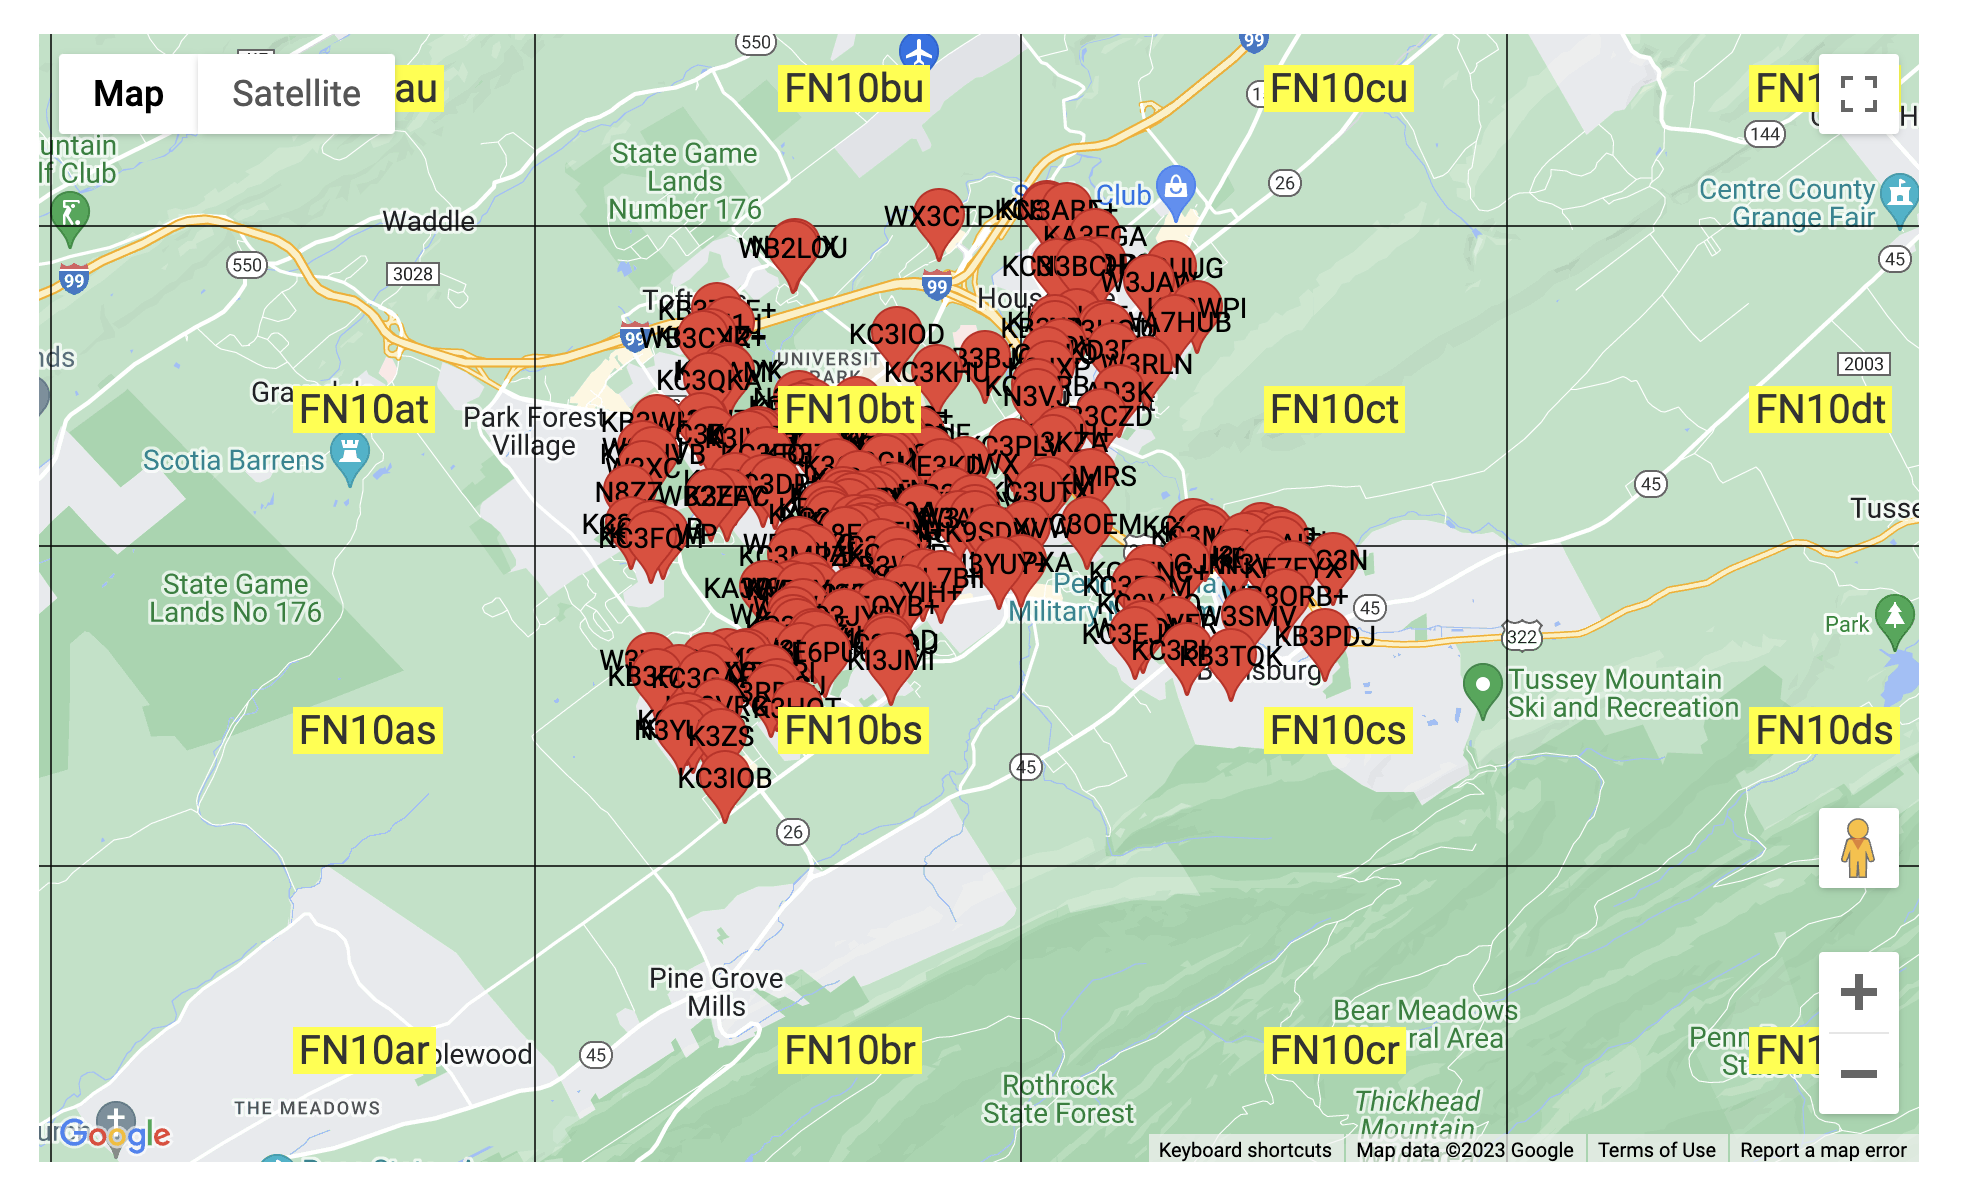
\includegraphics[width=1\textwidth,height=\textheight]{include/img/hams-in-16801.png}

}

\caption{Hams in Zip code 16801 from https://haminfo.tetranz.com/map}

\end{figure}

If you check the ``Show grid labels'' checkbox you will see that the map
shows the 6-character {[}grid square{]} designator. Some hams
``collect'' QSOs from different grid squares. Many hams operating
{[}FT8{]} or {[}FT4{]} exchange grid squares, as do those who operate
amateur satellites, see the
\protect\hyperlink{quest-satellites}{satellite quest}.

\hypertarget{search-for-a-specific-callsign}{%
\subsection*{Search for a specific
callsign}\label{search-for-a-specific-callsign}}
\addcontentsline{toc}{subsection}{Search for a specific callsign}

If you know a ham's callsign, enter it in the Callsign box.

Here is the map of licensed hams near to the mailing address for K3CR,
the Penn State Amateur Radio Club's callsign.

\begin{figure}

{\centering 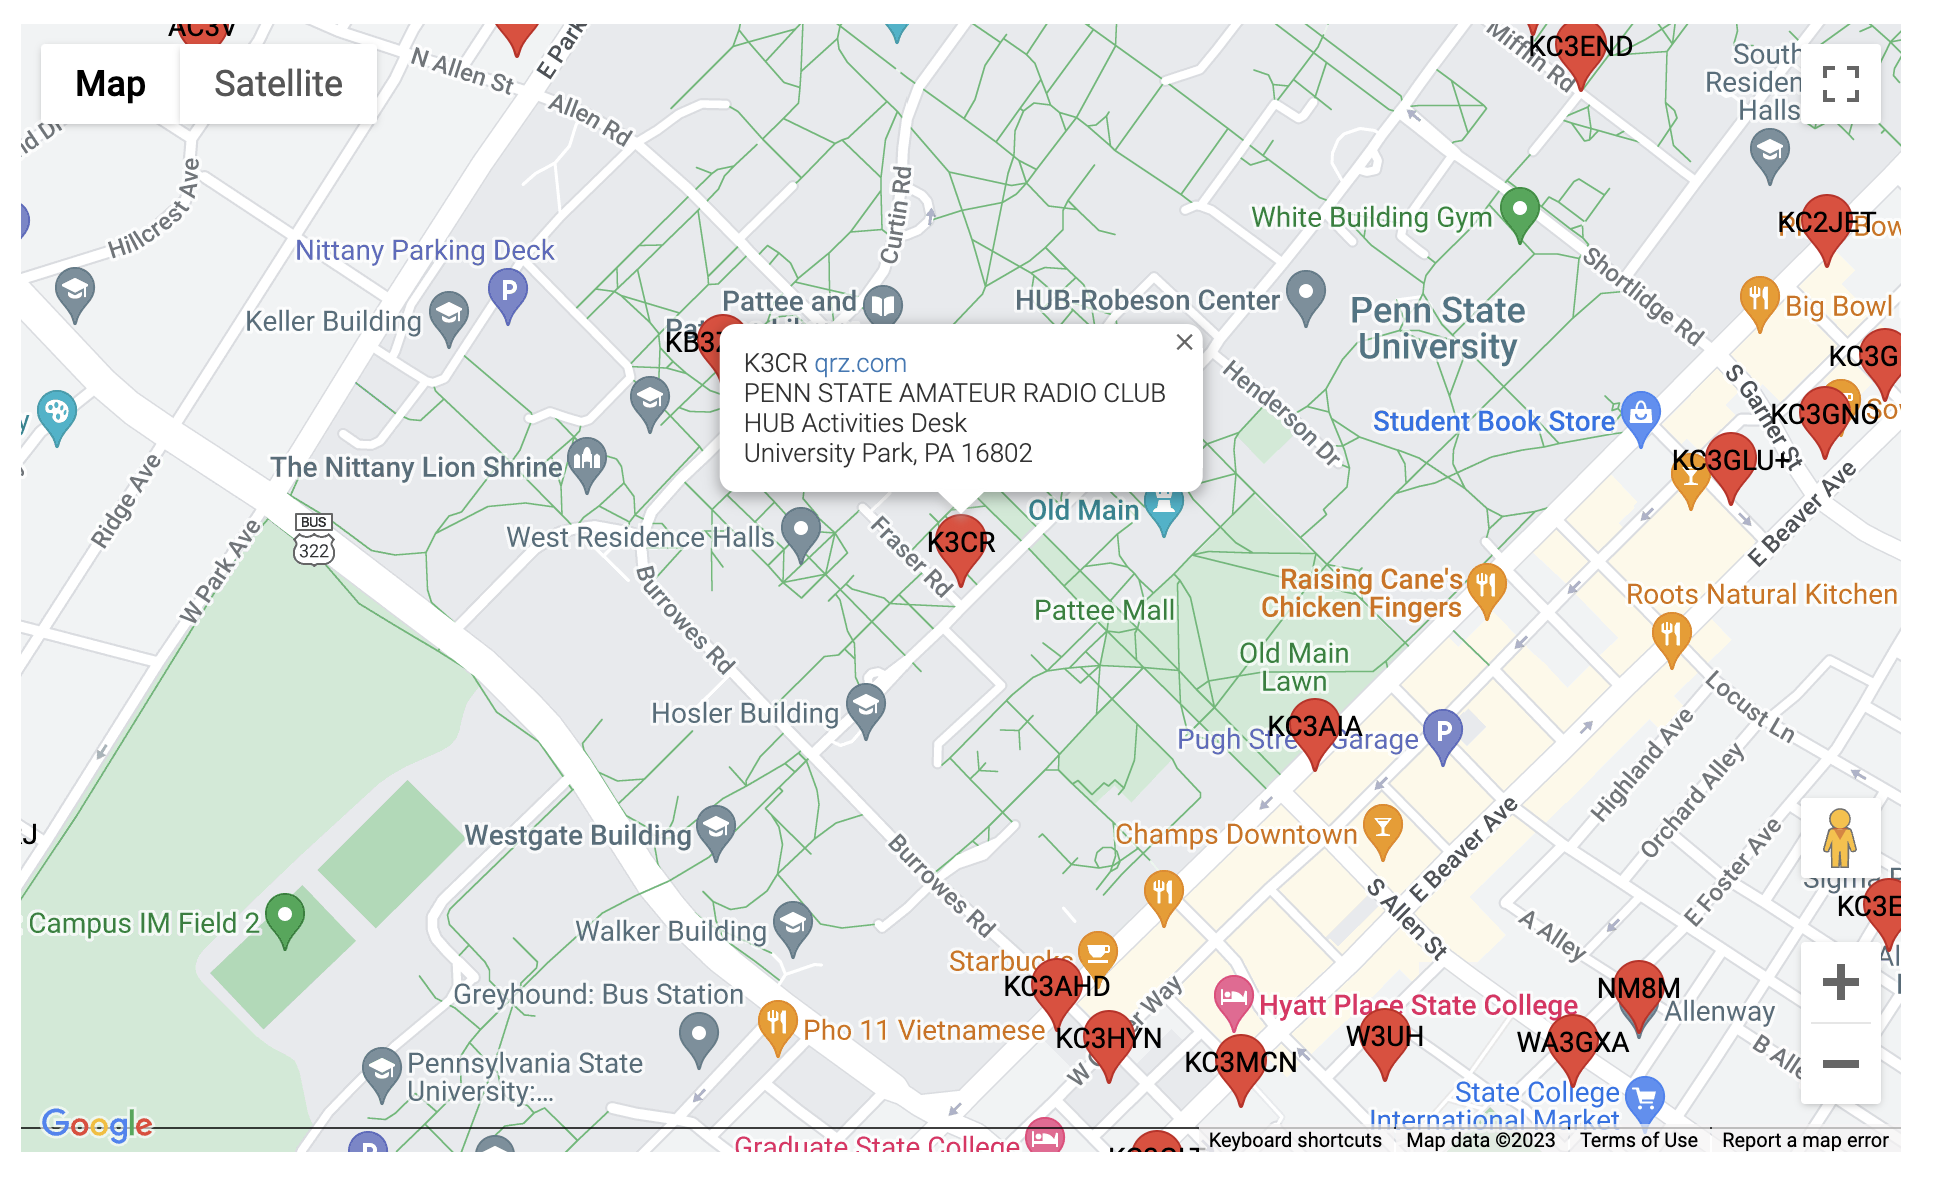
\includegraphics[width=1\textwidth,height=\textheight]{include/img/hams-near-k3cr.png}

}

\caption{Hams near K3CR from https://haminfo.tetranz.com/map}

\end{figure}

\begin{tcolorbox}[enhanced jigsaw, colframe=quarto-callout-note-color-frame, opacitybacktitle=0.6, colback=white, arc=.35mm, toprule=.15mm, bottomtitle=1mm, breakable, titlerule=0mm, toptitle=1mm, title=\textcolor{quarto-callout-note-color}{\faInfo}\hspace{0.5em}{Note}, rightrule=.15mm, coltitle=black, left=2mm, colbacktitle=quarto-callout-note-color!10!white, opacityback=0, bottomrule=.15mm, leftrule=.75mm]

You \emph{must} maintain a valid address with the FCC and that address
is public. Some hams who prefer not to have their physical address
publicly available rent a post office (PO) box and use that for their
address in the FCC database. This is perfectly acceptable.

\end{tcolorbox}

\hypertarget{quest-ham-geography}{%
\chapter*{Quest: Ham geography}\label{quest-ham-geography}}
\addcontentsline{toc}{chapter}{Quest: Ham geography}

\markboth{Quest: Ham geography}{Quest: Ham geography}

\hypertarget{about-4}{%
\section*{About}\label{about-4}}
\addcontentsline{toc}{section}{About}

\markright{About}

One of the great joys of ham radio is communicating with people in
different places. There are multiple ways to divide up the globe into
smaller chunks. In this quest, we'll explore some of the ways hams have
sliced up the global pie, geographically speaking. Each slice has its
use in ham radio.

See \url{https://www.mapability.com/ei8ic/maps/maps.php}

\hypertarget{itu-regions}{%
\section*{ITU Regions}\label{itu-regions}}
\addcontentsline{toc}{section}{ITU Regions}

\markright{ITU Regions}

\url{https://en.wikipedia.org/wiki/ITU_Region}

\begin{figure}

{\centering \includegraphics{index_files/mediabag/IARU_Regions_01.png}

}

\caption{ITU region map from
https://www.mapability.com/ei8ic/maps/regions.php}

\end{figure}

\hypertarget{itu-zones}{%
\section*{ITU Zones}\label{itu-zones}}
\addcontentsline{toc}{section}{ITU Zones}

\markright{ITU Zones}

\begin{figure}

{\centering \includegraphics{index_files/mediabag/ITU_Zones_ARRL_01.png}

}

\caption{ITU zones map from
https://www.mapability.com/ei8ic/maps/ituzone.php}

\end{figure}

\hypertarget{dx-entities}{%
\section*{DX Entities}\label{dx-entities}}
\addcontentsline{toc}{section}{DX Entities}

\markright{DX Entities}

ARRL: \url{http://www.arrl.org/country-lists-prefixes}

\url{https://www.ng3k.com/Dxcc/dxcc.html}

\hypertarget{cq-zones}{%
\section*{CQ Zones}\label{cq-zones}}
\addcontentsline{toc}{section}{CQ Zones}

\markright{CQ Zones}

\begin{figure}

{\centering \includegraphics{index_files/mediabag/CQ_Zones_01.png}

}

\caption{CQ Magazine zones map from
https://www.mapability.com/ei8ic/maps/cqzone.php}

\end{figure}

\hypertarget{callsign-areas}{%
\subsection*{Callsign areas}\label{callsign-areas}}
\addcontentsline{toc}{subsection}{Callsign areas}

\begin{figure}

{\centering \includegraphics{index_files/mediabag/USA_Call_Areas_1652.png}

}

\caption{USA callsign areas from
https://www.mapability.com/ei8ic/maps/usa\_call\_areas.php}

\end{figure}

\hypertarget{arrl-divisions}{%
\section*{ARRL divisions}\label{arrl-divisions}}
\addcontentsline{toc}{section}{ARRL divisions}

\markright{ARRL divisions}

\begin{figure}

{\centering \includegraphics{index_files/mediabag/ARRL_Divisions_1701.png}

}

\caption{ARRL divisions map from
https://www.mapability.com/ei8ic/maps/arrl\_divisions.php}

\end{figure}

\hypertarget{arrlrac-sections}{%
\subsection*{ARRL/RAC sections}\label{arrlrac-sections}}
\addcontentsline{toc}{subsection}{ARRL/RAC sections}

\begin{figure}

{\centering \includegraphics{index_files/mediabag/ARRL_RAC_Sections_20.png}

}

\caption{ARRL/RAC sections map from
https://www.mapability.com/ei8ic/maps/sections\_2.php}

\end{figure}

\hypertarget{summits-on-the-air}{%
\section*{Summits on the Air}\label{summits-on-the-air}}
\addcontentsline{toc}{section}{Summits on the Air}

\markright{Summits on the Air}

\hypertarget{parks-on-the-air}{%
\section*{Parks on the Air}\label{parks-on-the-air}}
\addcontentsline{toc}{section}{Parks on the Air}

\markright{Parks on the Air}

\hypertarget{maidenhead-locator}{%
\section*{Maidenhead Locator}\label{maidenhead-locator}}
\addcontentsline{toc}{section}{Maidenhead Locator}

\markright{Maidenhead Locator}

\url{https://en.wikipedia.org/wiki/Maidenhead_Locator_System\#:~:text=The\%20Maidenhead\%20Locator\%20System\%20(a.k.a.,was\%20limited\%20to\%20European\%20contacts}

By User:Denelson83 - \textless a rel=``nofollow'' class=``external
free''
href=``http://visibleearth.nasa.gov/view\_rec.php?id=2433''\textgreater http://visibleearth.nasa.gov/view\_rec.php?id=2433\textless/a\textgreater,
Public Domain, Link

\url{https://www.levinecentral.com/ham/grid_square.php?Call=K3CR}

\hypertarget{latitudelongitude}{%
\section*{Latitude/Longitude}\label{latitudelongitude}}
\addcontentsline{toc}{section}{Latitude/Longitude}

\markright{Latitude/Longitude}

\hypertarget{great-circle-maps}{%
\section*{Great Circle maps}\label{great-circle-maps}}
\addcontentsline{toc}{section}{Great Circle maps}

\markright{Great Circle maps}

\begin{figure}

{\centering \includegraphics{index_files/mediabag/washington_usa_great.png}

}

\caption{Great circle map centered on Washington, DC from
https://www.mapability.com/ei8ic/maps/great\_circle/capital\_cities/washington\_usa\_great\_circle\_map.php}

\end{figure}

\part{Gear}

\hypertarget{about-5}{%
\section*{About}\label{about-5}}
\addcontentsline{toc}{section}{About}

\markright{About}

We've shown that there are many ham-related activities that a person can
enjoy without buying any new gear. But of course, buying or borrowing
radio equipment dramatically expands what a ham or ham-to-be can do.
There's an old saying that if you ask two hams the same question about
what gear to buy, they'll give you three opinions, and you should ignore
all of them. Ok, so that's not much help.

In this short section, I'm going to give you a very opinionated take on
\emph{how you should think} about what gear to buy, not what specific
bit of equipment to buy.

But before doing that, here are some general observations:

\begin{itemize}
\tightlist
\item
  There is \emph{no} perfect (fill in the blank, i.e., radio, antenna,
  etc).
\item
  Most hams who remain active in the hobby end up with more than one
  radio.
\item
  Yes, older used equipment seems more expensive than it seems like it
  should be.
\end{itemize}

\hypertarget{planning}{%
\chapter*{Planning}\label{planning}}
\addcontentsline{toc}{chapter}{Planning}

\markboth{Planning}{Planning}

\hypertarget{about-6}{%
\section*{About}\label{about-6}}
\addcontentsline{toc}{section}{About}

\markright{About}

Before you spend a dollar, I suggest that you put some time into
planning the initial phases of your ham ``career''. Your interests will
probably change over time, but it's a good idea to start with what
excites you about the hobby right now. Here are some questions to
consider. None of them have either/or answers.

\hypertarget{questions}{%
\section*{Questions}\label{questions}}
\addcontentsline{toc}{section}{Questions}

\markright{Questions}

\begin{itemize}
\tightlist
\item
  \emph{Where} do you plan to operate?
\end{itemize}

From home, in your car, or from a portable location like a park or a
mountain summit?

\begin{itemize}
\tightlist
\item
  \emph{What mode or modes} do you want to operate in these places?
\end{itemize}

Voice (SSB or FM), digital modes, or CW?

\begin{itemize}
\tightlist
\item
  \emph{What type(s) of activities} interest you in using these modes?
\end{itemize}

Special event support, contesting, SOTA/POTA, rag-chewing, nets.

\begin{itemize}
\tightlist
\item
  \emph{Who} do you want to communicate with?
\end{itemize}

People you don't know (yet) or very specific individuals.

And last, but certainly not the least important:

\begin{itemize}
\tightlist
\item
  \emph{How much} do you have to spend?
\end{itemize}

In my opinion, the first question, \emph{where} you plan to operate, has
the biggest influence on your choices. So, what follows are three
separate chapters relating to setting up a fixed station at-home,
operating mobile (from a vehicle), and field or portable operations.

\part{FCC Regulations}

\hypertarget{part-97}{%
\chapter{FCC Part 97}\label{part-97}}

The following was downloaded as a
\href{include/pdf/47\%20CFR\%20Part\%2097\%20(up\%20to\%20date\%20as\%20of\%203-30-2023).pdf}{PDF}
from
\url{https://www.ecfr.gov/current/title-47/chapter-I/subchapter-D/part-97}
on 2023-04-01.

\begin{center}\rule{0.5\linewidth}{0.5pt}\end{center}

PART 97---AMATEUR RADIO SERVICE Authority:
\href{https://www.govinfo.gov/link/uscode/47/151}{47 U.S.C. 151}--155,
301--609, unless otherwise noted. Source:
\href{https://www.federalregister.gov/citation/54-FR-25857}{54 FR
25857}, June 20, 1989, unless otherwise noted.

\begin{tcolorbox}[enhanced jigsaw, colframe=quarto-callout-note-color-frame, opacitybacktitle=0.6, colback=white, arc=.35mm, toprule=.15mm, bottomtitle=1mm, breakable, titlerule=0mm, toptitle=1mm, title=\textcolor{quarto-callout-note-color}{\faInfo}\hspace{0.5em}{Note}, rightrule=.15mm, coltitle=black, left=2mm, colbacktitle=quarto-callout-note-color!10!white, opacityback=0, bottomrule=.15mm, leftrule=.75mm]

Editorial Note: Nomenclature changes to part 97 appear at 63 FR 54077,
Oct.~8, 1998.

\end{tcolorbox}

\hypertarget{subpart-A}{%
\section*{Subpart A---General Provisions}\label{subpart-A}}
\addcontentsline{toc}{section}{Subpart A---General Provisions}

\markright{Subpart A---General Provisions}

\hypertarget{97.1}{%
\subsection*{§ 97.1 Basis and purpose.}\label{97.1}}
\addcontentsline{toc}{subsection}{§ 97.1 Basis and purpose.}

The rules and regulations in this part are designed to provide an
amateur radio service having a fundamental purpose as expressed in the
following principles:

\begin{enumerate}
\def\labelenumi{(\alph{enumi})}
\item
  Recognition and enhancement of the value of the amateur service to the
  public as a voluntary noncommercial communication service,
  particularly with respect to providing emergency communications.
\item
  Continuation and extension of the amateur's proven ability to
  contribute to the advancement of the radio art.
\item
  Encouragement and improvement of the amateur service through rules
  which provide for advancing skills in both the communication and
  technical phases of the art.
\item
  Expansion of the existing reservoir within the amateur radio service
  of trained operators, technicians, and electronics experts.
\item
  Continuation and extension of the amateur's unique ability to enhance
  international goodwill.
\end{enumerate}

\hypertarget{97.3}{%
\subsection*{§ 97.3 Definitions.}\label{97.3}}
\addcontentsline{toc}{subsection}{§ 97.3 Definitions.}

\begin{enumerate}
\def\labelenumi{(\alph{enumi})}
\tightlist
\item
  The definitions of terms used in part 97 are:
\end{enumerate}

\begin{enumerate}
\def\labelenumi{(\arabic{enumi})}
\item
  \leavevmode\vadjust pre{\hypertarget{amateur-operator}{}}%
  Amateur operator. A person named in an amateur operator/primary
  license station grant on the ULS consolidated licensee database to be
  the control operator of an amateur station.
\item
  \leavevmode\vadjust pre{\hypertarget{amateur-radio-service}{}}%
  Amateur radio services. The amateur service, the amateur-satellite
  service and the radio amateur civil emergency service.
\item
  \leavevmode\vadjust pre{\hypertarget{amateur-service}{}}%
  Amateur service. A radiocommunication service for the purpose of
  self-training, intercommunication and technical investigations carried
  out by amateurs, that is, duly authorized persons interested in radio
  technique solely with a personal aim and without pecuniary interest.
\item
  \leavevmode\vadjust pre{\hypertarget{amateur-station}{}}%
  Amateur station. A station in an amateur radio service consisting of
  the apparatus necessary for carrying on radiocommunications.
\item
  \leavevmode\vadjust pre{\hypertarget{automatic-control}{}}%
  Automatic control. The use of devices and procedures for control of a
  station when it is transmitting so that compliance with the FCC Rules
  is achieved without the control operator being present at a control
  point.
\item
  \leavevmode\vadjust pre{\hypertarget{auxiliary-station}{}}%
  Auxiliary station. An amateur station, other than in a message
  forwarding system, that is transmitting communications point-to-point
  within a system of cooperating amateur stations.
\item
  \leavevmode\vadjust pre{\hypertarget{bandwidth}{}}%
  Bandwidth. The width of a frequency band outside of which the mean
  power of the transmitted signal is attenuated at least 26 dB below the
  mean power of the transmitted signal within the band.
\item
  \leavevmode\vadjust pre{\hypertarget{beacon}{}}%
  Beacon. An amateur station transmitting communications for the
  purposes of observation of propagation and reception or other related
  experimental activities.
\item
  \leavevmode\vadjust pre{\hypertarget{broadcasting}{}}%
  Broadcasting. Transmissions intended for reception by the general
  public, either direct or relayed.
\item
  Call sign system. The method used to select a call sign for amateur
  station over-the-air identification purposes. The call sign systems
  are:
\end{enumerate}

\begin{enumerate}
\def\labelenumi{(\roman{enumi})}
\item
  Sequential call sign system. The call sign is selected by the FCC from
  an alphabetized list corresponding to the geographic region of the
  licensee's mailing address and operator class. The call sign is shown
  on the license. The FCC will issue public announcements detailing the
  procedures of the sequential call sign system.
\item
  Vanity call sign system. The call sign is selected by the FCC from a
  list of call signs requested by the licensee. The call sign is shown
  on the license. The FCC will issue public announcements detailing the
  procedures of the vanity call sign system.
\item
  Special event call sign system. The call sign is selected by the
  station licensee from a list of call signs shown on a common data base
  coordinated, maintained and disseminated by the amateur station
  special event call sign data base coordinators. The call sign must
  have the single letter prefix K, N or W, followed by a single numeral
  0 through 9, followed by a single letter A through W or Y or Z (for
  example K1A). The special event call sign is substituted for the call
  sign shown on the station license grant while the station is
  transmitting. The FCC will issue public announcements detailing the
  procedures of the special event call sign system.
\end{enumerate}

\begin{enumerate}
\def\labelenumi{(\arabic{enumi})}
\setcounter{enumi}{11}
\item
  CEPT radio amateur license. A license issued by a country belonging to
  the European Conference of Postal and Telecommunications
  Administrations (CEPT) that has adopted Recommendation T/R 61--01
  (Nice 1985, Paris 1992, Nicosia 2003).
\item
  \leavevmode\vadjust pre{\hypertarget{control-operator}{}}%
  Control operator. An amateur operator designated by the licensee of a
  station to be responsible for the transmissions from that station to
  assure compliance with the FCC Rules.
\item
  \leavevmode\vadjust pre{\hypertarget{control-point}{}}%
  Control point. The location at which the control operator function is
  performed.
\item
  \leavevmode\vadjust pre{\hypertarget{CSCE}{}}%
  CSCE. Certificate of successful completion of an examination.
\item
  \leavevmode\vadjust pre{\hypertarget{earth-station}{}}%
  Earth station. An amateur station located on, or within 50 km of, the
  Earth's surface intended for communications with space stations or
  with other Earth stations by means of one or more other objects in
  space.
\item
  {[}Reserved{]}
\item
  External RF power amplifier. A device capable of increasing power
  output when used in conjunction with, but not an integral part of, a
  transmitter.
\item
  {[}Reserved{]}
\item
  FAA. Federal Aviation Administration.
\item
  FCC. Federal Communications Commission.
\item
  \leavevmode\vadjust pre{\hypertarget{frequency-coordinator}{}}%
  Frequency coordinator. An entity, recognized in a local or regional
  area by amateur operators whose stations are eligible to be auxiliary
  or repeater stations, that recommends transmit/receive channels and
  associated operating and technical parameters for such stations in
  order to avoid or minimize potential interference.
\item
  Harmful interference. Interference which endangers the functioning of
  a radionavigation service or of other safety services or seriously
  degrades, obstructs or repeatedly interrupts a radiocommunication
  service operating in accordance with the Radio Regulations.
\item
  IARP (International Amateur Radio Permit). A document issued pursuant
  to the terms of the Inter-American Convention on an International
  Amateur Radio Permit by a country signatory to that Convention, other
  than the United States. Montrouis, Haiti. AG/doc.3216/95.
\item
  Indicator. Words, letters or numerals appended to and separated from
  the call sign during the station identification.
\item
  Information bulletin. A message directed only to amateur operators
  consisting solely of subject matter of direct interest to the amateur
  service.
\item
  In-law. A parent, stepparent, sibling, or step-sibling of a licensee's
  spouse; the spouse of a licensee's sibling, step-sibling, child, or
  stepchild; or the spouse of a licensee's spouse's sibling or
  step-sibling.
\item
  International Morse code. A dot-dash code as defined in ITU--T
  Recommendation F.1 (March, 1998), Division B, I. Morse code.
\item
  ITU. International Telecommunication Union.
\item
  \leavevmode\vadjust pre{\hypertarget{line-A}{}}%
  Line A. Begins at Aberdeen, WA, running by great circle arc to the
  intersection of 48° N, 120° W, thence along parallel 48° N, to the
  intersection of 95° W, thence by great circle arc through the
  southernmost point of Duluth, MN, thence by great circle arc to 45° N,
  85° W, thence southward along meridian 85° W, to its intersection with
  parallel 41° N, thence along parallel 41° N, to its intersection with
  meridian 82° W, thence by great circle arc through the southernmost
  point of Bangor, ME, thence by great circle arc through the
  southernmost point of Searsport, ME, at which point it terminates.
\item
  \leavevmode\vadjust pre{\hypertarget{local-control}{}}%
  Local control. The use of a control operator who directly manipulates
  the operating adjustments in the station to achieve compliance with
  the FCC Rules.
\item
  Message forwarding system. A group of amateur stations participating
  in a voluntary, cooperative, interactive arrangement where
  communications are sent from the control operator of an originating
  station to the control operator of one or more destination stations by
  one or more forwarding stations.
\item
  National Radio Quiet Zone. The area in Maryland, Virginia and West
  Virginia Bounded by 39°15′ N on the north, 78°30′ W on the east,
  37°30′ N on the south and 80°30′ W on the west.
\item
  Physician. For the purpose of this part, a person who is licensed to
  practice in a place where the amateur service is regulated by the FCC,
  as either a Doctor of Medicine (M.D.) or a Doctor of Osteopathy (D.O.)
\item
  Question pool. All current examination questions for a designated
  written examination element.
\item
  Question set. A series of examination questions on a given examination
  selected from the question pool.
\item
  Radio Regulations. The latest ITU Radio Regulations to which the
  United States is a party.
\item
  \leavevmode\vadjust pre{\hypertarget{RACES}{}}%
  RACES (radio amateur civil emergency service). A radio service using
  amateur stations for civil defense communications during periods of
  local, regional or national civil emergencies.
\item
  \leavevmode\vadjust pre{\hypertarget{remote-control}{}}%
  Remote control. The use of a control operator who indirectly
  manipulates the operating adjustments in the station through a control
  link to achieve compliance with the FCC Rules.
\item
  \leavevmode\vadjust pre{\hypertarget{repeater}{}}%
  Repeater. An amateur station that simultaneously retransmits the
  transmission of another amateur station on a different channel or
  channels.
\item
  \leavevmode\vadjust pre{\hypertarget{space-station}{}}%
  Space station. An amateur station located more than 50 km above the
  Earth's surface.
\item
  Space telemetry. A one-way transmission from a space station of
  measurements made from the measuring instruments in a spacecraft,
  including those relating to the functioning of the spacecraft.
\item
  Spurious emission. An emission, or frequencies outside the necessary
  bandwidth of a transmission, the level of which may be reduced without
  affecting the information being transmitted.
\item
  Telecommand. A one-way transmission to initiate, modify, or terminate
  functions of a device at a distance.
\item
  Telecommand station. An amateur station that transmits communications
  to initiate, modify or terminate functions of a space station.
\item
  Telemetry. A one-way transmission of measurements at a distance from
  the measuring instrument.
\item
  \leavevmode\vadjust pre{\hypertarget{third-party-communications}{}}%
  Third party communications. A message from the control operator (first
  party) of an amateur station to another amateur station control
  operator (second party) on behalf of another person (third party).
\item
  ULS (Universal Licensing System). The consolidated database,
  application filing system and processing system for all Wireless
  Telecommunications Services.
\item
  VE. Volunteer examiner.
\item
  VEC. Volunteer-examiner coordinator.
\end{enumerate}

\begin{enumerate}
\def\labelenumi{(\alph{enumi})}
\setcounter{enumi}{1}
\tightlist
\item
  The definitions of technical symbols used in this part are:
\end{enumerate}

\begin{enumerate}
\def\labelenumi{(\arabic{enumi})}
\item
  EHF (extremely high frequency). The frequency range 30--300 GHz.
\item
  EIRP (equivalent isotropically radiated power). The product of the
  power supplied to the antenna and the antenna gain in a given
  direction relative to an isotropic antenna (absolute or isotropic
  gain).
\end{enumerate}

Note: Divide EIRP by 1.64 to convert to effective radiated power. (3)
ERP (effective radiated power) (in a given direction). The product of
the power supplied to the antenna and its gain relative to a half-wave
dipole in a given direction.

Note: Multiply ERP by 1.64 to convert to equivalent isotropically
radiated power. (4) HF (high frequency). The frequency range 3--30 MHz.

\begin{enumerate}
\def\labelenumi{(\arabic{enumi})}
\setcounter{enumi}{4}
\item
  Hz. Hertz.
\item
  LF (low frequency). The frequency range 30--300 kHz.
\item
  \begin{enumerate}
  \def\labelenumii{\alph{enumii}.}
  \setcounter{enumii}{12}
  \tightlist
  \item
    Meters.
  \end{enumerate}
\item
  MF (medium frequency). The frequency range 300--3000 kHz.
\item
  PEP (peak envelope power). The average power supplied to the antenna
  transmission line by a transmitter during one RF cycle at the crest of
  the modulation envelope taken under normal operating conditions.
\item
  RF. Radio frequency.
\item
  SHF (super high frequency). The frequency range 3--30 GHz.
\item
  UHF (ultra high frequency). The frequency range 300--3000 MHz.
\item
  VHF (very high frequency). The frequency range 30--300 MHz.
\item
  W. Watts.
\end{enumerate}

\begin{enumerate}
\def\labelenumi{(\alph{enumi})}
\setcounter{enumi}{2}
\tightlist
\item
  The following terms are used in this part to indicate emission types.
  Refer to § 2.201 of the FCC Rules, Emission, modulation and
  transmission characteristics, for information on emission type
  designators.
\end{enumerate}

\begin{itemize}
\item
  \begin{enumerate}
  \def\labelenumi{(\arabic{enumi})}
  \tightlist
  \item
    CW. International Morse code telegraphy emissions having designators
    with A, C, H, J or R as the first symbol; 1 as the second symbol; A
    or B as the third symbol; and emissions J2A and J2B.
  \end{enumerate}
\item
  \begin{enumerate}
  \def\labelenumi{(\arabic{enumi})}
  \setcounter{enumi}{1}
  \tightlist
  \item
    Data. Telemetry, telecommand and computer communications emissions
    having
  \end{enumerate}

  \begin{itemize}
  \item
    \begin{enumerate}
    \def\labelenumi{(\roman{enumi})}
    \tightlist
    \item
      designators with A, C, D, F, G, H, J or R as the first symbol, 1
      as the second symbol, and D as the third symbol;
    \end{enumerate}
  \item
    \begin{enumerate}
    \def\labelenumi{(\roman{enumi})}
    \setcounter{enumi}{1}
    \tightlist
    \item
      emission J2D; and
    \end{enumerate}
  \item
    \begin{enumerate}
    \def\labelenumi{(\roman{enumi})}
    \setcounter{enumi}{2}
    \tightlist
    \item
      emissions A1C, F1C, F2C, J2C, and J3C having an occupied bandwidth
      of 500 Hz or less when transmitted on an amateur service frequency
      below 30 MHz. Only a digital code of a type specifically
      authorized in this part may be transmitted.
    \end{enumerate}
  \end{itemize}
\item
  \begin{enumerate}
  \def\labelenumi{(\arabic{enumi})}
  \setcounter{enumi}{2}
  \tightlist
  \item
    Image. Facsimile and television emissions having designators with A,
    C, D, F, G, H, J or R as the first symbol; 1, 2 or 3 as the second
    symbol; C or F as the third symbol; and emissions having B as the
    first symbol; 7, 8 or 9 as the second symbol; W as the third symbol.
  \end{enumerate}
\item
  \begin{enumerate}
  \def\labelenumi{(\arabic{enumi})}
  \setcounter{enumi}{3}
  \tightlist
  \item
    MCW. Tone-modulated international Morse code telegraphy emissions
    having designators with A, C, D, F, G, H or R as the first symbol; 2
    as the second symbol; A or B as the third symbol.
  \end{enumerate}
\item
  \begin{enumerate}
  \def\labelenumi{(\arabic{enumi})}
  \setcounter{enumi}{4}
  \tightlist
  \item
    Phone. Speech and other sound emissions having designators with A,
    C, D, F, G, H, J or R as the first symbol; 1, 2, 3 or X as the
    second symbol; E as the third symbol. Also speech emissions having B
    or F as the first symbol; 7, 8 or 9 as the second symbol; E as the
    third symbol. MCW for the purpose of performing the station
    identification procedure, or for providing telegraphy practice
    interspersed with speech. Incidental tones for the purpose of
    selective calling or alerting or to control the level of a
    demodulated signal may also be considered phone.
  \end{enumerate}
\item
  \begin{enumerate}
  \def\labelenumi{(\arabic{enumi})}
  \setcounter{enumi}{5}
  \tightlist
  \item
    Pulse. Emissions having designators with K, L, M, P, Q, V or W as
    the first symbol; 0, 1, 2, 3, 7, 8, 9 or X as the second symbol; A,
    B, C, D, E, F, N, W or X as the third symbol.
  \end{enumerate}
\item
  \begin{enumerate}
  \def\labelenumi{(\arabic{enumi})}
  \setcounter{enumi}{6}
  \tightlist
  \item
    RTTY. Narrow-band direct-printing telegraphy emissions having
    designators with A, C, D, F, G, H, J or R as the first symbol; 1 as
    the second symbol; B as the third symbol; and emission J2B. Only a
    digital code of a type specifically authorized in this part may be
    transmitted.
  \end{enumerate}
\item
  \begin{enumerate}
  \def\labelenumi{(\arabic{enumi})}
  \setcounter{enumi}{7}
  \tightlist
  \item
    SS. Spread spectrum emissions using bandwidth-expansion modulation
    emissions having designators with A, C, D, F, G, H, J or R as the
    first symbol; X as the second symbol; X as the third symbol.
  \end{enumerate}
\item
  \begin{enumerate}
  \def\labelenumi{(\arabic{enumi})}
  \setcounter{enumi}{8}
  \tightlist
  \item
    Test. Emissions containing no information having the designators
    with N as the third symbol. Test does not include pulse emissions
    with no information or modulation unless pulse emissions are also
    authorized in the frequency band.
  \end{enumerate}
\end{itemize}

{[}54 FR 25857, June 20, 1989{]}

EDITORIAL NOTE Editorial Note: For Federal Register citations affecting
§ 97.3, see the List of CFR Sections Affected, which appears in the
Finding Aids section of the printed volume and at www.govinfo.gov.

\hypertarget{97.5}{%
\subsection*{§ 97.5 Station license required.}\label{97.5}}
\addcontentsline{toc}{subsection}{§ 97.5 Station license required.}

\begin{enumerate}
\def\labelenumi{(\alph{enumi})}
\tightlist
\item
  The station apparatus must be under the physical control of a person
  named in an amateur station license grant on the ULS consolidated
  license database or a person authorized for alien reciprocal operation
  by § 97.107 of this part, before the station may transmit on any
  amateur service frequency from any place that is:
\end{enumerate}

\begin{itemize}
\item
  \begin{enumerate}
  \def\labelenumi{(\arabic{enumi})}
  \tightlist
  \item
    Within 50 km of the Earth's surface and at a place where the amateur
    service is regulated by the FCC;
  \end{enumerate}
\item
  \begin{enumerate}
  \def\labelenumi{(\arabic{enumi})}
  \setcounter{enumi}{1}
  \tightlist
  \item
    Within 50 km of the Earth's surface and aboard any vessel or craft
    that is documented or registered in the United States; or
  \end{enumerate}
\item
  \begin{enumerate}
  \def\labelenumi{(\arabic{enumi})}
  \setcounter{enumi}{2}
  \tightlist
  \item
    More than 50 km above the Earth's surface aboard any craft that is
    documented or registered in the United States.
  \end{enumerate}
\end{itemize}

\begin{enumerate}
\def\labelenumi{(\alph{enumi})}
\setcounter{enumi}{1}
\tightlist
\item
  The types of station license grants are:
\end{enumerate}

\begin{itemize}
\item
  \begin{enumerate}
  \def\labelenumi{(\arabic{enumi})}
  \tightlist
  \item
    An operator/primary station license grant. One, but only one,
    operator/primary station license grant may be held by any one
    person. The primary station license is granted together with the
    amateur operator license. Except for a representative of a foreign
    government, any person who qualifies by examination is eligible to
    apply for an operator/primary station license grant.
  \end{enumerate}
\item
  \begin{enumerate}
  \def\labelenumi{(\arabic{enumi})}
  \setcounter{enumi}{1}
  \tightlist
  \item
    A club station license grant. A club station license grant may be
    held only by the person who is the license trustee designated by an
    officer of the club. The trustee must be a person who holds an
    operator/primary station license grant. The club must be composed of
    at least four persons and must have a name, a document of
    organization, management, and a primary purpose devoted to amateur
    service activities consistent with this part.
  \end{enumerate}
\item
  \begin{enumerate}
  \def\labelenumi{(\arabic{enumi})}
  \setcounter{enumi}{2}
  \tightlist
  \item
    A military recreation station license grant. A military recreation
    station license grant may be held only by the person who is the
    license custodian designated by the official in charge of the United
    States military recreational premises where the station is situated.
    The person must not be a representative of a foreign government. The
    person need not hold an amateur operator license grant.
  \end{enumerate}
\end{itemize}

\begin{enumerate}
\def\labelenumi{(\alph{enumi})}
\setcounter{enumi}{2}
\item
  The person named in the station license grant or who is authorized for
  alien reciprocal operation by § 97.107 of this part may use, in
  accordance with the applicable rules of this part, the transmitting
  apparatus under the physical control of the person at places where the
  amateur service is regulated by the FCC.
\item
  A CEPT radio-amateur license is issued to the person by the country of
  which the person is a citizen. The person must not:
\end{enumerate}

\begin{itemize}
\item
  \begin{enumerate}
  \def\labelenumi{(\arabic{enumi})}
  \tightlist
  \item
    Be a resident alien or citizen of the United States, regardless of
    any other citizenship also held;
  \end{enumerate}
\item
  \begin{enumerate}
  \def\labelenumi{(\arabic{enumi})}
  \setcounter{enumi}{1}
  \tightlist
  \item
    Hold an FCC-issued amateur operator license nor reciprocal permit
    for alien amateur licensee;
  \end{enumerate}
\item
  \begin{enumerate}
  \def\labelenumi{(\arabic{enumi})}
  \setcounter{enumi}{2}
  \tightlist
  \item
    Be a prior amateur service licensee whose FCC-issued license was
    revoked, suspended for less than the balance of the license term and
    the suspension is still in effect, suspended for the balance of the
    license term and relicensing has not taken place, or surrendered for
    cancellation following notice of revocation, suspension or monetary
    forfeiture proceedings; or
  \end{enumerate}
\item
  \begin{enumerate}
  \def\labelenumi{(\arabic{enumi})}
  \setcounter{enumi}{3}
  \tightlist
  \item
    Be the subject of a cease and desist order that relates to amateur
    service operation and which is still in effect.
  \end{enumerate}
\end{itemize}

\begin{enumerate}
\def\labelenumi{(\alph{enumi})}
\setcounter{enumi}{4}
\tightlist
\item
  An IARP is issued to the person by the country of which the person is
  a citizen. The person must not:
\end{enumerate}

\begin{itemize}
\item
  \begin{enumerate}
  \def\labelenumi{(\arabic{enumi})}
  \tightlist
  \item
    Be a resident alien or citizen of the United States, regardless of
    any other citizenship also held;
  \end{enumerate}
\item
  \begin{enumerate}
  \def\labelenumi{(\arabic{enumi})}
  \setcounter{enumi}{1}
  \tightlist
  \item
    Hold an FCC-issued amateur operator license nor reciprocal permit
    for alien amateur licensee;
  \end{enumerate}
\item
  \begin{enumerate}
  \def\labelenumi{(\arabic{enumi})}
  \setcounter{enumi}{2}
  \tightlist
  \item
    Be a prior amateur service licensee whose FCC-issued license was
    revoked, suspended for less than the balance of the license term and
    the suspension is still in effect, suspended for the balance of the
    license term and relicensing has not taken place, or surrendered for
    cancellation following notice of revocation, suspension or monetary
    forfeiture proceedings; or
  \end{enumerate}
\item
  \begin{enumerate}
  \def\labelenumi{(\arabic{enumi})}
  \setcounter{enumi}{3}
  \tightlist
  \item
    Be the subject of a cease and desist order that relates to amateur
    service operation and which is still in effect.
  \end{enumerate}
\end{itemize}

{[}59 FR 54831, Nov.~2, 1994, as amended at 62 FR 17567, Apr.~10, 1997;
63 FR 68977, Dec.~14, 1998; 75 FR 78169, Dec.~15, 2010{]}

\hypertarget{97.7}{%
\subsection*{§ 97.7 Control operator required.}\label{97.7}}
\addcontentsline{toc}{subsection}{§ 97.7 Control operator required.}

When transmitting, each amateur station must have a control operator.
The control operator must be a person:

\begin{enumerate}
\def\labelenumi{(\alph{enumi})}
\item
  For whom an amateur operator/primary station license grant appears on
  the ULS consolidated licensee database, or
\item
  Who is authorized for alien reciprocal operation by § 97.107 of this
  part.
\end{enumerate}

{[}63 FR 68978, Dec.~14, 1998{]}

\hypertarget{97.9}{%
\subsection*{§ 97.9 Operator license grant.}\label{97.9}}
\addcontentsline{toc}{subsection}{§ 97.9 Operator license grant.}

\begin{enumerate}
\def\labelenumi{(\alph{enumi})}
\item
  The classes of amateur operator license grants are: Novice,
  Technician, General, Advanced, and Amateur Extra. The person named in
  the operator license grant is authorized to be the control operator of
  an amateur station with the privileges authorized to the operator
  class specified on the license grant.
\item
  The person named in an operator license grant of Novice, Technician,
  General or Advanced Class, who has properly submitted to the
  administering VEs a FCC Form 605 document requesting examination for
  an operator license grant of a higher class, and who holds a CSCE
  indicating that the person has completed the necessary examinations
  within the previous 365 days, is authorized to exercise the rights and
  privileges of the higher operator class until final disposition of the
  application or until 365 days following the passing of the
  examination, whichever comes first.
\end{enumerate}

{[}75 FR 78169, Dec.~15, 2010{]}

\hypertarget{97.11}{%
\subsection*{§ 97.11 Stations aboard ships or aircraft.}\label{97.11}}
\addcontentsline{toc}{subsection}{§ 97.11 Stations aboard ships or
aircraft.}

\begin{enumerate}
\def\labelenumi{(\alph{enumi})}
\item
  The installation and operation of an amateur station on a ship or
  aircraft must be approved by the master of the ship or pilot in
  command of the aircraft.
\item
  The station must be separate from and independent of all other radio
  apparatus installed on the ship or aircraft, except a common antenna
  may be shared with a voluntary ship radio installation. The station's
  transmissions must not cause interference to any other apparatus
  installed on the ship or aircraft.
\item
  The station must not constitute a hazard to the safety of life or
  property. For a station aboard an aircraft, the apparatus shall not be
  operated while the aircraft is operating under Instrument Flight
  Rules, as defined by the FAA, unless the station has been found to
  comply with all applicable FAA Rules.
\end{enumerate}

\hypertarget{restrictions-on-station-location.}{%
\subsection*{§ 97.13 Restrictions on station
location.}\label{restrictions-on-station-location.}}
\addcontentsline{toc}{subsection}{§ 97.13 Restrictions on station
location.}

\begin{enumerate}
\def\labelenumi{(\alph{enumi})}
\item
  Before placing an amateur station on land of environmental importance
  or that is significant in American history, architecture or culture,
  the licensee may be required to take certain actions prescribed by §§
  1.1305--1.1319 of this chapter.
\item
  A station within 1600 m (1 mile) of an FCC monitoring facility must
  protect that facility from harmful interference. Failure to do so
  could result in imposition of operating restrictions upon the amateur
  station pursuant to § 97.121. Geographical coordinates of the
  facilities that require protection are listed in § 0.121(c) of this
  chapter.
\item
  Before causing or allowing an amateur station to transmit from any
  place where the operation of the station could cause human exposure to
  RF electromagnetic field levels in excess of those allowed under §
  1.1310 of this chapter, the licensee is required to take certain
  actions.
\end{enumerate}

\begin{itemize}
\item
  \begin{enumerate}
  \def\labelenumi{(\arabic{enumi})}
  \tightlist
  \item
    The licensee shall ensure compliance with the Commission's radio
    frequency exposure requirements in §§ 1.1307(b), 2.1091, and 2.1093
    of this chapter, where applicable. In lieu of evaluation with the
    general population/uncontrolled exposure limits, amateur licensees
    may evaluate their operation with respect to members of his or her
    immediate household using the occupational/controlled exposure
    limits in § 1.1310, provided appropriate training and information
    has been accessed by the amateur licensee and members of his/her
    household. RF exposure of other nearby persons who are not members
    of the amateur licensee's household must be evaluated with respect
    to the general population/uncontrolled exposure limits. Appropriate
    methodologies and guidance for evaluating amateur radio service
    operation is described in the Office of Engineering and Technology
    (OET) Bulletin 65, Supplement B.
  \end{enumerate}
\item
  \begin{enumerate}
  \def\labelenumi{(\arabic{enumi})}
  \setcounter{enumi}{1}
  \tightlist
  \item
    If the routine environmental evaluation indicates that the RF
    electromagnetic fields could exceed the limits contained in § 1.1310
    of this chapter in accessible areas, the licensee must take action
    to prevent human exposure to such RF electromagnetic fields. Further
    information on evaluating compliance with these limits can be found
    in the FCC's OET Bulletin Number 65, ``Evaluating Compliance with
    FCC Guidelines for Human Exposure to Radiofrequency Electromagnetic
    Fields.''
  \end{enumerate}
\end{itemize}

{[}54 FR 25857, June 20, 1989, as amended at 55 FR 20398, May 16, 1990;
61 FR 41019, Aug.~7, 1996; 62 FR 47963, Sept.~12, 1997; 62 FR 49557,
Sept.~22, 1997; 62 FR 61448, Nov.~18, 1997; 63 FR 68978, Dec.~14, 1998;
65 FR 6549, Feb.~10, 2000; 80 FR 53752, Sept.~8, 2015; 85 FR 18151,
Apr.~1, 2020{]}

\hypertarget{station-antenna-structures.}{%
\subsection*{§ 97.15 Station antenna
structures.}\label{station-antenna-structures.}}
\addcontentsline{toc}{subsection}{§ 97.15 Station antenna structures.}

\begin{enumerate}
\def\labelenumi{(\alph{enumi})}
\item
  Owners of certain antenna structures more than 60.96 meters (200 feet)
  above ground level at the site or located near or at a public use
  airport must notify the Federal Aviation Administration and register
  with the Commission as required by part 17 of this chapter.
\item
  Except as otherwise provided herein, a station antenna structure may
  be erected at heights and dimensions sufficient to accommodate amateur
  service communications. (State and local regulation of a station
  antenna structure must not preclude amateur service communications.
  Rather, it must reasonably accommodate such communications and must
  constitute the minimum practicable regulation to accomplish the state
  or local authority's legitimate purpose. See PRB--1, 101 FCC 2d 952
  (1985) for details.)
\item
  Antennas used to transmit in the 2200 m and 630 m bands must not
  exceed 60 meters in height above ground level.
\end{enumerate}

{[}64 FR 53242, Oct.~1, 1999, as amended at 82 FR 27214, June 14,
2017{]}

\hypertarget{97.17}{%
\subsection*{§ 97.17 Application for new license grant.}\label{97.17}}
\addcontentsline{toc}{subsection}{§ 97.17 Application for new license
grant.}

\begin{enumerate}
\def\labelenumi{(\alph{enumi})}
\item
  Any qualified person is eligible to apply for a new operator/primary
  station, club station or military recreation station license grant. No
  new license grant will be issued for a Novice or Advanced Class
  operator/primary station.
\item
  Each application for a new amateur service license grant must be filed
  with the FCC as follows:
\end{enumerate}

\begin{itemize}
\item
  \begin{enumerate}
  \def\labelenumi{(\arabic{enumi})}
  \tightlist
  \item
    Each candidate for an amateur radio operator license which requires
    the applicant to pass one or more examination elements must present
    the administering VEs with all information required by the rules
    prior to the examination. The VEs may collect all necessary
    information in any manner of their choosing, including creating
    their own forms.
  \end{enumerate}
\item
  \begin{enumerate}
  \def\labelenumi{(\arabic{enumi})}
  \setcounter{enumi}{1}
  \tightlist
  \item
    For a new club or military recreation station license grant, each
    applicant must present all information required by the rules to an
    amateur radio organization having tax-exempt status under section
    501(c)(3) of the Internal Revenue Code of 1986 that provides
    voluntary, uncompensated and unreimbursed services in providing club
    and military recreation station call signs (``Club Station Call Sign
    Administrator'') who must submit the information to the FCC in an
    electronic batch file. The Club Station Call Sign Administrator may
    collect the information required by these rules in any manner of
    their choosing, including creating their own forms. The Club Station
    Call Sign Administrator must retain the applicants information for
    at least 15 months and make it available to the FCC upon request.
    The FCC will issue public announcements listing the qualified
    organizations that have completed a pilot autogrant batch filing
    project and are authorized to serve as a Club Station Call Sign
    Administrator.
  \end{enumerate}
\item
  \begin{enumerate}
  \def\labelenumi{(\alph{enumi})}
  \setcounter{enumi}{2}
  \tightlist
  \item
    No person shall obtain or attempt to obtain, or assist another
    person to obtain or attempt to obtain, an amateur service license
    grant by fraudulent means.
  \end{enumerate}
\item
  \begin{enumerate}
  \def\labelenumi{(\alph{enumi})}
  \setcounter{enumi}{3}
  \tightlist
  \item
    One unique call sign will be shown on the license grant of each new
    primary, club and military recreation station. The call sign will be
    selected by the sequential call sign system. Effective February 14,
    2011, no club station license grants will be issued to a licensee
    who is shown as the license trustee on an existing club station
    license grant.
  \end{enumerate}
\end{itemize}

{[}63 FR 68978, Dec.~14, 1998, as amended at 64 FR 53242, Oct.~1, 1999;
65 FR 6549, Feb.~10, 2000; 75 FR 78170, Dec.~15, 2010{]}

\hypertarget{application-for-a-vanity-call-sign.}{%
\subsection*{§ 97.19 Application for a vanity call
sign.}\label{application-for-a-vanity-call-sign.}}
\addcontentsline{toc}{subsection}{§ 97.19 Application for a vanity call
sign.}

\begin{enumerate}
\def\labelenumi{(\alph{enumi})}
\item
  The person named in an operator/primary station license grant or in a
  club station license grant is eligible to make application for
  modification of the license grant, or the renewal thereof, to show a
  call sign selected by the vanity call sign system. Effective February
  14, 2011, the person named in a club station license grant that shows
  on the license a call sign that was selected by a trustee is not
  eligible for an additional vanity call sign. (The person named in a
  club station license grant that shows on the license a call sign that
  was selected by a trustee is eligible for a vanity call sign for his
  or her operator/primary station license grant on the same basis as any
  other person who holds an operator/primary station license grant.)
  Military recreation stations are not eligible for a vanity call sign.
\item
  Each application for a modification of an operator/primary or club
  station license grant, or the renewal thereof, to show a call sign
  selected by the vanity call sign system must be filed in accordance
  with § 1.913 of this chapter.
\item
  Unassigned call signs are available to the vanity call sign system
  with the following exceptions:
\end{enumerate}

\begin{itemize}
\item
  \begin{enumerate}
  \def\labelenumi{(\arabic{enumi})}
  \tightlist
  \item
    A call sign shown on an expired license grant is not available to
    the vanity call sign system for 2 years following the expiration of
    the license.
  \end{enumerate}
\item
  \begin{enumerate}
  \def\labelenumi{(\arabic{enumi})}
  \setcounter{enumi}{1}
  \tightlist
  \item
    A call sign shown on a surrendered or canceled license grant (except
    for a license grant that is canceled pursuant to § 97.31) is not
    available to the vanity call sign system for 2 years following the
    date such action is taken. (The availability of a call sign shown on
    a license canceled pursuant to § 97.31 is governed by paragraph
    (c)(3) of this section.)
  \end{enumerate}

  \begin{itemize}
  \item
    \begin{enumerate}
    \def\labelenumi{(\roman{enumi})}
    \tightlist
    \item
      This 2-year period does not apply to any license grant pursuant to
      paragraph (c)(3)(i), (ii), or (iii) of this section that is
      surrendered, canceled, revoked, voided, or set aside because the
      grantee acknowledged or the Commission determined that the grantee
      was not eligible for the exception. In such a case, the call sign
      is not available to the vanity call sign system for 30 days
      following the date such action is taken, or for the period for
      which the call sign would not have been available to the vanity
      call sign system pursuant to paragraphs (c)(2) or (3) of this
      section but for the intervening grant to the ineligible applicant,
      whichever is later.
    \end{enumerate}
  \item
    \begin{enumerate}
    \def\labelenumi{(\roman{enumi})}
    \setcounter{enumi}{1}
    \tightlist
    \item
      An applicant to whose operator/primary station license grant, or
      club station license grant for which the applicant is the trustee,
      the call sign was previously assigned is exempt from the 2-year
      period set forth in paragraph (c)(2) of this section.
    \end{enumerate}
  \end{itemize}
\item
  \begin{enumerate}
  \def\labelenumi{(\arabic{enumi})}
  \setcounter{enumi}{2}
  \tightlist
  \item
    A call sign shown on a license canceled pursuant to § 97.31 of this
    part is not available to the vanity call sign system for 2 years
    following the person's death, or for 2 years following the
    expiration of the license grant, whichever is sooner. If, however, a
    license is canceled more than 2 years after the licensee's death (or
    within 30 days before the second anniversary of the licensee's
    death), the call sign is not available to the vanity call sign
    system for 30 days following the date such action is taken. The
    following applicants are exempt from this 2-year period:
  \end{enumerate}

  \begin{itemize}
  \item
    \begin{enumerate}
    \def\labelenumi{(\roman{enumi})}
    \tightlist
    \item
      An applicant to whose operator/primary station license grant, or
      club station license grant for which the applicant is the trustee,
      the call sign was previously assigned; or
    \end{enumerate}
  \item
    \begin{enumerate}
    \def\labelenumi{(\roman{enumi})}
    \setcounter{enumi}{1}
    \tightlist
    \item
      An applicant who is the spouse, child, grandchild, stepchild,
      parent, grandparent, stepparent, brother, sister, stepbrother,
      stepsister, aunt, uncle, niece, nephew, or in-law of the person
      now deceased or of any other deceased former holder of the call
      sign, provided that the vanity call sign requested by the
      applicant is from the group of call signs corresponding to the
      same or lower class of operator license held by the applicant as
      designated in the sequential call sign system; or
    \end{enumerate}
  \item
    \begin{enumerate}
    \def\labelenumi{(\roman{enumi})}
    \setcounter{enumi}{2}
    \tightlist
    \item
      An applicant who is a club station license trustee acting with a
      written statement of consent signed by either the licensee ante
      mortem but who is now deceased, or by at least one relative as
      listed in paragraph (c)(3)(ii) of this section, of the person now
      deceased or of any other deceased former holder of the call sign,
      provided that the deceased former holder was a member of the club
      during his or her life.
    \end{enumerate}
  \end{itemize}
\end{itemize}

\begin{enumerate}
\def\labelenumi{(\alph{enumi})}
\setcounter{enumi}{3}
\tightlist
\item
  The vanity call sign requested by an applicant must be selected from
  the group of call signs corresponding to the same or lower class of
  operator license held by the applicant as designated in the sequential
  call sign system.
\end{enumerate}

\begin{itemize}
\item
  \begin{enumerate}
  \def\labelenumi{(\arabic{enumi})}
  \tightlist
  \item
    The applicant must request that the call sign shown on the license
    grant be vacated and provide a list of up to 25 call signs in order
    of preference. In the event that the Commission receives more than
    one application requesting a vanity call sign from an applicant on
    the same receipt day, the Commission will process only the first
    such application entered into the Universal Licensing System.
    Subsequent vanity call sign applications from that applicant with
    the same receipt date will not be accepted.
  \end{enumerate}
\item
  \begin{enumerate}
  \def\labelenumi{(\arabic{enumi})}
  \setcounter{enumi}{1}
  \tightlist
  \item
    The first assignable call sign from the applicant's list will be
    shown on the license grant. When none of those call signs are
    assignable, the call sign vacated by the applicant will be shown on
    the license grant.
  \end{enumerate}
\item
  \begin{enumerate}
  \def\labelenumi{(\arabic{enumi})}
  \setcounter{enumi}{2}
  \tightlist
  \item
    Vanity call signs will be selected from those call signs assignable
    at the time the application is processed by the FCC.
  \end{enumerate}
\item
  \begin{enumerate}
  \def\labelenumi{(\arabic{enumi})}
  \setcounter{enumi}{3}
  \tightlist
  \item
    A call sign designated under the sequential call sign system for
    Alaska, Hawaii, Caribbean Insular Areas, and Pacific Insular areas
    will be assigned only to a primary or club station whose licensee's
    mailing address is in the corresponding state, commonwealth, or
    island. This limitation does not apply to an applicant for the call
    sign as the spouse, child, grandchild, stepchild, parent,
    grandparent, stepparent, brother, sister, stepbrother, stepsister,
    aunt, uncle, niece, nephew, or in-law, of the former holder now
    deceased.
  \end{enumerate}
\end{itemize}

{[}60 FR 7460, Feb.~8, 1995, as amended at 60 FR 50123, Sept.~28, 1995;
60 FR 53132, Oct.~12, 1995; 63 FR 68979, Dec.~14, 1998; 71 FR 66461,
Nov.~15, 2006; 75 FR 78170, Dec.~15, 2010{]}

\hypertarget{97.21}{%
\subsection*{§ 97.21 Application for a modified or renewed license
grant.}\label{97.21}}
\addcontentsline{toc}{subsection}{§ 97.21 Application for a modified or
renewed license grant.}

\begin{enumerate}
\def\labelenumi{(\alph{enumi})}
\tightlist
\item
  A person holding a valid amateur station license grant:
\end{enumerate}

\begin{itemize}
\item
  \begin{enumerate}
  \def\labelenumi{(\arabic{enumi})}
  \tightlist
  \item
    Must apply to the FCC for a modification of the license grant as
    necessary to show the correct mailing and email address, licensee
    name, club name, license trustee name, or license custodian name in
    accordance with § 1.913 of this chapter. For a club or military
    recreation station license grant, the application must be presented
    in document form to a Club Station Call Sign Administrator who must
    submit the information thereon to the FCC in an electronic batch
    file. The Club Station Call Sign Administrator must retain the
    collected information for at least 15 months and make it available
    to the FCC upon request. A Club Station Call Sign Administrator
    shall not file with the Commission any application to modify a club
    station license grant that was submitted by a person other than the
    trustee as shown on the license grant, except an application to
    change the club station license trustee. An application to modify a
    club station license grant to change the license trustee name must
    be submitted to a Club Station Call Sign Administrator and must be
    signed by an officer of the club.
  \end{enumerate}
\item
  \begin{enumerate}
  \def\labelenumi{(\arabic{enumi})}
  \setcounter{enumi}{1}
  \tightlist
  \item
    May apply to the FCC for a modification of the operator/primary
    station license grant to show a higher operator class. Applicants
    must present the administering VEs with all information required by
    the rules prior to the examination. The VEs may collect all
    necessary information in any manner of their choosing, including
    creating their own forms.
  \end{enumerate}
\item
  \begin{enumerate}
  \def\labelenumi{(\arabic{enumi})}
  \setcounter{enumi}{2}
  \tightlist
  \item
    May apply to the FCC for renewal of the license grant for another
    term in accordance with §§ 1.913 and 1.949 of this chapter.
    Application for renewal of a Technician Plus Class operator/primary
    station license will be processed as an application for renewal of a
    Technician Class operator/primary station license.
  \end{enumerate}

  \begin{itemize}
  \item
    \begin{enumerate}
    \def\labelenumi{(\roman{enumi})}
    \tightlist
    \item
      For a station license grant showing a call sign obtained through
      the vanity call sign system, the application must be filed in
      accordance with § 97.19 of this part in order to have the vanity
      call sign reassigned to the station.
    \end{enumerate}
  \item
    \begin{enumerate}
    \def\labelenumi{(\roman{enumi})}
    \setcounter{enumi}{1}
    \tightlist
    \item
      For a primary station license grant showing a call sign obtained
      through the sequential call sign system, and for a primary station
      license grant showing a call sign obtained through the vanity call
      sign system but whose grantee does not want to have the vanity
      call sign reassigned to the station, the application must be filed
      with the FCC in accordance with § 1.913 of this chapter. When the
      application has been received by the FCC on or before the license
      expiration date, the license operating authority is continued
      until the final disposition of the application.
    \end{enumerate}
  \item
    \begin{enumerate}
    \def\labelenumi{(\roman{enumi})}
    \setcounter{enumi}{2}
    \tightlist
    \item
      For a club station or military recreation station license grant
      showing a call sign obtained through the sequential call sign
      system, and for a club station license grant showing a call sign
      obtained through the vanity call sign system but whose grantee
      does not want to have the vanity call sign reassigned to the
      station, the application must be presented in document form to a
      Club Station Call Sign Administrator who must submit the
      information thereon to the FCC in an electronic batch file. The
      replacement call sign will be selected by the sequential call sign
      system. The Club Station Call Sign Administrator must retain the
      collected information for at least 15 months and make it available
      to the FCC upon request.
    \end{enumerate}
  \end{itemize}
\end{itemize}

\begin{enumerate}
\def\labelenumi{(\alph{enumi})}
\setcounter{enumi}{1}
\item
  A person whose amateur station license grant has expired may apply to
  the FCC for renewal of the license grant for another term during a 2
  year filing grace period. The application must be received at the
  address specified above prior to the end of the grace period. Unless
  and until the license grant is renewed, no privileges in this part are
  conferred.
\item
  Except as provided in paragraph (a)(3) of this section, a call sign
  obtained under the sequential or vanity call sign system will be
  reassigned to the station upon renewal or modification of a station
  license.
\end{enumerate}

{[}63 FR 68979, Dec.~14, 1998, as amended at 64 FR 53242, Oct.~1, 1999;
65 FR 6550, Feb.~10, 2000; 75 FR 78170, Dec.~15, 2010; 79 FR 35291, July
21, 2014; 85 FR 85532, Dec.~29, 2020{]}

\hypertarget{97.23}{%
\subsection*{§ 97.23 Mailing and email addresses.}\label{97.23}}
\addcontentsline{toc}{subsection}{§ 97.23 Mailing and email addresses.}

Each license grant must show the grantee's correct name, mailing
address, and email address. The email address must be an address where
the grantee can receive electronic correspondence. Revocation of the
station license or suspension of the operator license may result when
correspondence from the FCC is returned as undeliverable because the
grantee failed to provide the correct email address.

{[}85 FR 85533, Dec.~29, 2020{]}

\hypertarget{97.25}{%
\subsection*{§ 97.25 License term.}\label{97.25}}
\addcontentsline{toc}{subsection}{§ 97.25 License term.}

An amateur service license is normally granted for a 10-year term.

{[}63 FR 68979, Dec.~14, 1998{]}

\hypertarget{fcc-modification-of-station-license-grant.}{%
\subsection{§ 97.27 FCC modification of station license
grant.}\label{fcc-modification-of-station-license-grant.}}

\begin{enumerate}
\def\labelenumi{(\alph{enumi})}
\tightlist
\item
  The FCC may modify a station license grant, either for a limited time
  or for the duration of the term thereof, if it determines:
\end{enumerate}

\begin{itemize}
\item
  \begin{enumerate}
  \def\labelenumi{(\arabic{enumi})}
  \tightlist
  \item
    That such action will promote the public interest, convenience, and
    necessity; or
  \end{enumerate}
\item
  \begin{enumerate}
  \def\labelenumi{(\arabic{enumi})}
  \setcounter{enumi}{1}
  \tightlist
  \item
    That such action will promote fuller compliance with the provisions
    of the Communications Act of 1934, as amended, or of any treaty
    ratified by the United States.
  \end{enumerate}
\end{itemize}

\begin{enumerate}
\def\labelenumi{(\alph{enumi})}
\setcounter{enumi}{1}
\tightlist
\item
  When the FCC makes such a determination, it will issue an order of
  modification. The order will not become final until the licensee is
  notified in writing of the proposed action and the grounds and reasons
  therefor. The licensee will be given reasonable opportunity of no less
  than 30 days to protest the modification; except that, where safety of
  life or property is involved, a shorter period of notice may be
  provided. Any protest by a licensee of an FCC order of modification
  will be handled in accordance with the provisions of 47 U.S.C. 316.
\end{enumerate}

{[}59 FR 54833, Nov.~2, 1994, as amended at 63 FR 68979, Dec.~14,
1998{]}

\hypertarget{replacement-license-grant-document.}{%
\subsection*{§ 97.29 Replacement license grant
document.}\label{replacement-license-grant-document.}}
\addcontentsline{toc}{subsection}{§ 97.29 Replacement license grant
document.}

Each grantee whose amateur station license grant document is lost,
mutilated or destroyed may apply to the FCC for a replacement in
accordance with § 1.913 of this chapter.

{[}63 FR 68979, Dec.~14, 1998{]}

\hypertarget{cancellation-on-account-of-the-licensees-death.}{%
\subsection*{§ 97.31 Cancellation on account of the licensee's
death.}\label{cancellation-on-account-of-the-licensees-death.}}
\addcontentsline{toc}{subsection}{§ 97.31 Cancellation on account of the
licensee's death.}

\begin{enumerate}
\def\labelenumi{(\alph{enumi})}
\item
  A person may request cancellation of an operator/primary station
  license grant on account of the licensee's death by submitting a
  signed request that includes a death certificate, obituary, or Social
  Security Death Index data that shows the person named in the
  operator/primary station license grant has died. Such a request may be
  submitted as a pleading associated with the deceased licensee's
  license. See § 1.45 of this chapter. In addition, the Commission may
  cancel an operator/primary station license grant if it becomes aware
  of the grantee's death through other means. No action will be taken
  during the last thirty days of the post-expiration grace period (see §
  97.21(b)) on a request to cancel a license due to the licensee's
  death.
\item
  A license that is canceled due to the licensee's death is canceled as
  of the date of the licensee's death.
\end{enumerate}

{[}75 FR 78171, Dec.~15, 2010{]}

\hypertarget{subpart-bstation-operation-standards}{%
\section*{Subpart B---Station Operation
Standards}\label{subpart-bstation-operation-standards}}
\addcontentsline{toc}{section}{Subpart B---Station Operation Standards}

\markright{Subpart B---Station Operation Standards}

\hypertarget{97.101}{%
\subsection*{§ 97.101 General standards.}\label{97.101}}
\addcontentsline{toc}{subsection}{§ 97.101 General standards.}

\begin{enumerate}
\def\labelenumi{(\alph{enumi})}
\item
  In all respects not specifically covered by FCC Rules each amateur
  station must be operated in accordance with good engineering and good
  amateur practice.
\item
  Each station licensee and each control operator must cooperate in
  selecting transmitting channels and in making the most effective use
  of the amateur service frequencies. No frequency will be assigned for
  the exclusive use of any station.
\item
  At all times and on all frequencies, each control operator must give
  priority to stations providing emergency communications, except to
  stations transmitting communications for training drills and tests in
  RACES.
\item
  No amateur operator shall willfully or maliciously interfere with or
  cause interference to any radio communication or signal.
\end{enumerate}

\hypertarget{station-licensee-responsibilities.}{%
\subsection*{§ 97.103 Station licensee
responsibilities.}\label{station-licensee-responsibilities.}}
\addcontentsline{toc}{subsection}{§ 97.103 Station licensee
responsibilities.}

\begin{enumerate}
\def\labelenumi{(\alph{enumi})}
\item
  The station licensee is responsible for the proper operation of the
  station in accordance with the FCC Rules. When the control operator is
  a different amateur operator than the station licensee, both persons
  are equally responsible for proper operation of the station.
\item
  The station licensee must designate the station control operator. The
  FCC will presume that the station licensee is also the control
  operator, unless documentation to the contrary is in the station
  records.
\item
  The station licensee must make the station and the station records
  available for inspection upon request by an FCC representative.
\end{enumerate}

{[}54 FR 25857, June 20, 1989, as amended at 71 FR 66462, Nov.~15, 2006;
75 FR 27201, May 14, 2010{]}

\hypertarget{control-operator-duties.}{%
\subsection*{§ 97.105 Control operator
duties.}\label{control-operator-duties.}}
\addcontentsline{toc}{subsection}{§ 97.105 Control operator duties.}

\begin{enumerate}
\def\labelenumi{(\alph{enumi})}
\item
  The control operator must ensure the immediate proper operation of the
  station, regardless of the type of control.
\item
  A station may only be operated in the manner and to the extent
  permitted by the privileges authorized for the class of operator
  license held by the control operator.
\end{enumerate}

\hypertarget{reciprocal-operating-authority.}{%
\subsection*{§ 97.107 Reciprocal operating
authority.}\label{reciprocal-operating-authority.}}
\addcontentsline{toc}{subsection}{§ 97.107 Reciprocal operating
authority.}

A non-citizen of the United States (``alien'') holding an amateur
service authorization granted by the alien's government is authorized to
be the control operator of an amateur station located at places where
the amateur service is regulated by the FCC, provided there is in effect
a multilateral or bilateral reciprocal operating arrangement, to which
the United States and the alien's government are parties, for amateur
service operation on a reciprocal basis. The FCC will issue public
announcements listing the countries with which the United States has
such an arrangement. No citizen of the United States or person holding
an FCC amateur operator/primary station license grant is eligible for
the reciprocal operating authority granted by this section. The
privileges granted to a control operator under this authorization are:

\begin{enumerate}
\def\labelenumi{(\alph{enumi})}
\tightlist
\item
  For an amateur service license granted by the Government of Canada:
\end{enumerate}

\begin{itemize}
\item
  \begin{enumerate}
  \def\labelenumi{(\arabic{enumi})}
  \tightlist
  \item
    The terms of the Convention Between the United States and Canada
    (TIAS No.~2508) Relating to the Operation by Citizens of Either
    Country of Certain Radio Equipment or Stations in the Other Country;
  \end{enumerate}
\item
  \begin{enumerate}
  \def\labelenumi{(\arabic{enumi})}
  \setcounter{enumi}{1}
  \tightlist
  \item
    The operating terms and conditions of the amateur service license
    issued by the Government of Canada; and
  \end{enumerate}
\item
  \begin{enumerate}
  \def\labelenumi{(\arabic{enumi})}
  \setcounter{enumi}{2}
  \tightlist
  \item
    The applicable rules of this part, but not to exceed the control
    operator privileges of an FCC-granted Amateur Extra Class operator
    license.
  \end{enumerate}
\end{itemize}

\begin{enumerate}
\def\labelenumi{(\alph{enumi})}
\setcounter{enumi}{1}
\tightlist
\item
  For an amateur service license granted by any country, other than
  Canada, with which the United States has a multilateral or bilateral
  agreement:
\end{enumerate}

\begin{itemize}
\item
  \begin{enumerate}
  \def\labelenumi{(\arabic{enumi})}
  \tightlist
  \item
    The terms of the agreement between the alien's government and the
    United States;
  \end{enumerate}
\item
  \begin{enumerate}
  \def\labelenumi{(\arabic{enumi})}
  \setcounter{enumi}{1}
  \tightlist
  \item
    The operating terms and conditions of the amateur service license
    granted by the alien's government;
  \end{enumerate}
\item
  \begin{enumerate}
  \def\labelenumi{(\arabic{enumi})}
  \setcounter{enumi}{2}
  \tightlist
  \item
    The applicable rules of this part, but not to exceed the control
    operator privileges of an FCC-granted Amateur Extra Class operator
    license; and
  \end{enumerate}
\end{itemize}

\begin{enumerate}
\def\labelenumi{(\alph{enumi})}
\setcounter{enumi}{2}
\tightlist
\item
  At any time the FCC may, in its discretion, modify, suspend or cancel
  the reciprocal operating authority granted to any person by this
  section.
\end{enumerate}

{[}63 FR 68979, Dec.~14, 1998{]}

\hypertarget{station-control.}{%
\subsection*{§ 97.109 Station control.}\label{station-control.}}
\addcontentsline{toc}{subsection}{§ 97.109 Station control.}

\begin{enumerate}
\def\labelenumi{(\alph{enumi})}
\item
  Each amateur station must have at least one control point.
\item
  When a station is being locally controlled, the control operator must
  be at the control point. Any station may be locally controlled.
\item
  When a station is being remotely controlled, the control operator must
  be at the control point. Any station may be remotely controlled.
\item
  When a station is being automatically controlled, the control operator
  need not be at the control point. Only stations specifically
  designated elsewhere in this part may be automatically controlled.
  Automatic control must cease upon notification by a Regional Director
  that the station is transmitting improperly or causing harmful
  interference to other stations. Automatic control must not be resumed
  without prior approval of the Regional Director.
\end{enumerate}

{[}54 FR 39535, Sept.~27, 1989, as amended at 60 FR 26001, May 16, 1995;
69 FR 24997, May 5, 2004; 80 FR 53753, Sept.~8, 2015{]}

\hypertarget{97.111}{%
\subsection*{§ 97.111 Authorized transmissions.}\label{97.111}}
\addcontentsline{toc}{subsection}{§ 97.111 Authorized transmissions.}

\begin{enumerate}
\def\labelenumi{(\alph{enumi})}
\tightlist
\item
  An amateur station may transmit the following types of two-way
  communications:
\end{enumerate}

\begin{itemize}
\item
  \begin{enumerate}
  \def\labelenumi{(\arabic{enumi})}
  \tightlist
  \item
    Transmissions necessary to exchange messages with other stations in
    the amateur service, except those in any country whose
    administration has notified the ITU that it objects to such
    communications. The FCC will issue public notices of current
    arrangements for international communications.
  \end{enumerate}
\item
  \begin{enumerate}
  \def\labelenumi{(\arabic{enumi})}
  \setcounter{enumi}{1}
  \tightlist
  \item
    Transmissions necessary to meet essential communication needs and to
    facilitate relief actions.
  \end{enumerate}
\item
  \begin{enumerate}
  \def\labelenumi{(\arabic{enumi})}
  \setcounter{enumi}{2}
  \tightlist
  \item
    Transmissions necessary to exchange messages with a station in
    another FCC-regulated service while providing emergency
    communications;
  \end{enumerate}
\item
  \begin{enumerate}
  \def\labelenumi{(\arabic{enumi})}
  \setcounter{enumi}{3}
  \tightlist
  \item
    Transmissions necessary to exchange messages with a United States
    government station, necessary to providing communications in RACES;
    and
  \end{enumerate}
\item
  \begin{enumerate}
  \def\labelenumi{(\arabic{enumi})}
  \setcounter{enumi}{4}
  \tightlist
  \item
    Transmissions necessary to exchange messages with a station in a
    service not regulated by the FCC, but authorized by the FCC to
    communicate with amateur stations. An amateur station may exchange
    messages with a participating United States military station during
    an Armed Forces Day Communications Test.
  \end{enumerate}
\end{itemize}

\begin{enumerate}
\def\labelenumi{(\alph{enumi})}
\setcounter{enumi}{1}
\tightlist
\item
  In addition to one-way transmissions specifically authorized elsewhere
  in this part, an amateur station may transmit the following types of
  one-way communications:
\end{enumerate}

\begin{itemize}
\item
  \begin{enumerate}
  \def\labelenumi{(\arabic{enumi})}
  \tightlist
  \item
    Brief transmissions necessary to make adjustments to the station;
  \end{enumerate}
\item
  \begin{enumerate}
  \def\labelenumi{(\arabic{enumi})}
  \setcounter{enumi}{1}
  \tightlist
  \item
    Brief transmissions necessary to establishing two-way communications
    with other stations;
  \end{enumerate}
\item
  \begin{enumerate}
  \def\labelenumi{(\arabic{enumi})}
  \setcounter{enumi}{2}
  \tightlist
  \item
    Telecommand;
  \end{enumerate}
\item
  \begin{enumerate}
  \def\labelenumi{(\arabic{enumi})}
  \setcounter{enumi}{3}
  \tightlist
  \item
    Transmissions necessary to providing emergency communications;
  \end{enumerate}
\item
  \begin{enumerate}
  \def\labelenumi{(\arabic{enumi})}
  \setcounter{enumi}{4}
  \tightlist
  \item
    Transmissions necessary to assisting persons learning, or improving
    proficiency in, the international Morse code; and
  \end{enumerate}
\item
  \begin{enumerate}
  \def\labelenumi{(\arabic{enumi})}
  \setcounter{enumi}{5}
  \tightlist
  \item
    Transmissions necessary to disseminate information bulletins.
  \end{enumerate}
\item
  \begin{enumerate}
  \def\labelenumi{(\arabic{enumi})}
  \setcounter{enumi}{6}
  \tightlist
  \item
    Transmissions of telemetry.
  \end{enumerate}
\end{itemize}

{[}54 FR 25857, June 20, 1989, as amended at 56 FR 56171, Nov.~1, 1991;
71 FR 25982, May 3, 2006; 71 FR 66462, Nov.~15, 2006{]}

\hypertarget{97.113}{%
\subsection*{§ 97.113 Prohibited transmissions.}\label{97.113}}
\addcontentsline{toc}{subsection}{§ 97.113 Prohibited transmissions.}

\begin{enumerate}
\def\labelenumi{(\alph{enumi})}
\tightlist
\item
  No amateur station shall transmit:
\end{enumerate}

\begin{itemize}
\item
  \begin{enumerate}
  \def\labelenumi{(\arabic{enumi})}
  \tightlist
  \item
    Communications specifically prohibited elsewhere in this part;
  \end{enumerate}
\item
  \begin{enumerate}
  \def\labelenumi{(\arabic{enumi})}
  \setcounter{enumi}{1}
  \tightlist
  \item
    Communications for hire or for material compensation, direct or
    indirect, paid or promised, except as otherwise provided in these
    rules;
  \end{enumerate}
\item
  \begin{enumerate}
  \def\labelenumi{(\arabic{enumi})}
  \setcounter{enumi}{2}
  \tightlist
  \item
    Communications in which the station licensee or control operator has
    a pecuniary interest, including communications on behalf of an
    employer, with the following exceptions:
  \end{enumerate}

  \begin{itemize}
  \item
    \begin{enumerate}
    \def\labelenumi{(\roman{enumi})}
    \tightlist
    \item
      A station licensee or station control operator may participate on
      behalf of an employer in an emergency preparedness or disaster
      readiness test or drill, limited to the duration and scope of such
      test or drill, and operational testing immediately prior to such
      test or drill. Tests or drills that are not government-sponsored
      are limited to a total time of one hour per week; except that no
      more than twice in any calendar year, they may be conducted for a
      period not to exceed 72 hours.
    \end{enumerate}
  \item
    \begin{enumerate}
    \def\labelenumi{(\roman{enumi})}
    \setcounter{enumi}{1}
    \tightlist
    \item
      An amateur operator may notify other amateur operators of the
      availability for sale or trade of apparatus normally used in an
      amateur station, provided that such activity is not conducted on a
      regular basis.
    \end{enumerate}
  \item
    \begin{enumerate}
    \def\labelenumi{(\roman{enumi})}
    \setcounter{enumi}{2}
    \tightlist
    \item
      A control operator may accept compensation as an incident of a
      teaching position during periods of time when an amateur station
      is used by that teacher as a part of classroom instruction at an
      educational institution.
    \end{enumerate}
  \item
    \begin{enumerate}
    \def\labelenumi{(\roman{enumi})}
    \setcounter{enumi}{3}
    \tightlist
    \item
      The control operator of a club station may accept compensation for
      the periods of time when the station is transmitting telegraphy
      practice or information bulletins, provided that the station
      transmits such telegraphy practice and bulletins for at least 40
      hours per week; schedules operations on at least six amateur
      service MF and HF bands using reasonable measures to maximize
      coverage; where the schedule of normal operating times and
      frequencies is published at least 30 days in advance of the actual
      transmissions; and where the control operator does not accept any
      direct or indirect compensation for any other service as a control
      operator.
    \end{enumerate}
  \end{itemize}
\item
  \begin{enumerate}
  \def\labelenumi{(\arabic{enumi})}
  \setcounter{enumi}{3}
  \tightlist
  \item
    Music using a phone emission except as specifically provided
    elsewhere in this section; communications intended to facilitate a
    criminal act; messages encoded for the purpose of obscuring their
    meaning, except as otherwise provided herein; obscene or indecent
    words or language; or false or deceptive messages, signals or
    identification.
  \end{enumerate}
\item
  \begin{enumerate}
  \def\labelenumi{(\arabic{enumi})}
  \setcounter{enumi}{4}
  \tightlist
  \item
    Communications, on a regular basis, which could reasonably be
    furnished alternatively through other radio services.
  \end{enumerate}
\end{itemize}

\begin{enumerate}
\def\labelenumi{(\alph{enumi})}
\setcounter{enumi}{1}
\item
  An amateur station shall not engage in any form of broadcasting, nor
  may an amateur station transmit one-way communications except as
  specifically provided in these rules; nor shall an amateur station
  engage in any activity related to program production or news gathering
  for broadcasting purposes, except that communications directly related
  to the immediate safety of human life or the protection of property
  may be provided by amateur stations to broadcasters for dissemination
  to the public where no other means of communication is reasonably
  available before or at the time of the event.
\item
  No station shall retransmit programs or signals emanating from any
  type of radio station other than an amateur station, except
  propagation and weather forecast information intended for use by the
  general public and originated from United States Government stations,
  and communications, including incidental music, originating on United
  States Government frequencies between a manned spacecraft and its
  associated Earth stations. Prior approval for manned spacecraft
  communications retransmissions must be obtained from the National
  Aeronautics and Space Administration. Such retransmissions must be for
  the exclusive use of amateur radio operators. Propagation, weather
  forecasts, and manned spacecraft communications retransmissions may
  not be conducted on a regular basis, but only occasionally, as an
  incident of normal amateur radio communications.
\item
  No amateur station, except an auxiliary, repeater, or space station,
  may automatically retransmit the radio signals of other amateur
  station.
\end{enumerate}

{[}58 FR 43072, Aug.~13, 1993; 58 FR 47219, Sept.~8, 1993, as amended at
71 FR 25982, May 3, 2006; 71 FR 66462, Nov.~15, 2006; 75 FR 46857,
Aug.~4, 2010; 79 FR 35291, June 20, 2014{]}

\hypertarget{third-party-communications.}{%
\subsection*{§ 97.115 Third party
communications.}\label{third-party-communications.}}
\addcontentsline{toc}{subsection}{§ 97.115 Third party communications.}

\begin{enumerate}
\def\labelenumi{(\alph{enumi})}
\tightlist
\item
  An amateur station may transmit messages for a third party to:
\end{enumerate}

\begin{itemize}
\item
  \begin{enumerate}
  \def\labelenumi{(\arabic{enumi})}
  \tightlist
  \item
    Any station within the jurisdiction of the United States.
  \end{enumerate}
\item
  \begin{enumerate}
  \def\labelenumi{(\arabic{enumi})}
  \setcounter{enumi}{1}
  \tightlist
  \item
    Any station within the jurisdiction of any foreign government when
    transmitting emergency or disaster relief communications and any
    station within the jurisdiction of any foreign government whose
    administration has made arrangements with the United States to allow
    amateur stations to be used for transmitting international
    communications on behalf of third parties. No station shall transmit
    messages for a third party to any station within the jurisdiction of
    any foreign government whose administration has not made such an
    arrangement. This prohibition does not apply to a message for any
    third party who is eligible to be a control operator of the station.
  \end{enumerate}
\end{itemize}

\begin{enumerate}
\def\labelenumi{(\alph{enumi})}
\setcounter{enumi}{1}
\tightlist
\item
  The third party may participate in stating the message where:
\end{enumerate}

\begin{itemize}
\item
  \begin{enumerate}
  \def\labelenumi{(\arabic{enumi})}
  \tightlist
  \item
    The control operator is present at the control point and is
    continuously monitoring and supervising the third party's
    participation; and
  \end{enumerate}
\item
  \begin{enumerate}
  \def\labelenumi{(\arabic{enumi})}
  \setcounter{enumi}{1}
  \tightlist
  \item
    The third party is not a prior amateur service licensee whose
    license was revoked or not renewed after hearing and re-licensing
    has not taken place; suspended for less than the balance of the
    license term and the suspension is still in effect; suspended for
    the balance of the license term and re-licensing has not taken
    place; or surrendered for cancellation following notice of
    revocation, suspension or monetary forfeiture proceedings. The third
    party may not be the subject of a cease and desist order which
    relates to amateur service operation and which is still in effect.
  \end{enumerate}
\end{itemize}

\begin{enumerate}
\def\labelenumi{(\alph{enumi})}
\setcounter{enumi}{2}
\item
  No station may transmit third party communications while being
  automatically controlled except a station transmitting a RTTY or data
  emission.
\item
  At the end of an exchange of international third party communications,
  the station must also transmit in the station identification procedure
  the call sign of the station with which a third party message was
  exchanged.
\end{enumerate}

{[}54 FR 25857, June 20, 1989; 54 FR 39535, Sept.~27, 1989, as amended
at 71 FR 25982, May 3, 2006; 71 FR 66462, Nov.~15, 2006{]}

\hypertarget{97.117}{%
\subsection*{§ 97.117 International communications.}\label{97.117}}
\addcontentsline{toc}{subsection}{§ 97.117 International
communications.}

Transmissions to a different country, where permitted, shall be limited
to communications incidental to the purposes of the amateur service and
to remarks of a personal character.

{[}71 FR 25982, May 3, 2006{]}

\hypertarget{97.119}{%
\subsection*{§ 97.119 Station identification.}\label{97.119}}
\addcontentsline{toc}{subsection}{§ 97.119 Station identification.}

\begin{enumerate}
\def\labelenumi{(\alph{enumi})}
\item
  Each amateur station, except a space station or telecommand station,
  must transmit its assigned call sign on its transmitting channel at
  the end of each communication, and at least every 10 minutes during a
  communication, for the purpose of clearly making the source of the
  transmissions from the station known to those receiving the
  transmissions. No station may transmit unidentified communications or
  signals, or transmit as the station call sign, any call sign not
  authorized to the station.
\item
  The call sign must be transmitted with an emission authorized for the
  transmitting channel in one of the following ways:
\end{enumerate}

\begin{itemize}
\item
  \begin{enumerate}
  \def\labelenumi{(\arabic{enumi})}
  \tightlist
  \item
    By a CW emission. When keyed by an automatic device used only for
    identification, the speed must not exceed 20 words per minute;
  \end{enumerate}
\item
  \begin{enumerate}
  \def\labelenumi{(\arabic{enumi})}
  \setcounter{enumi}{1}
  \tightlist
  \item
    By a phone emission in the English language. Use of a
    \protect\hyperlink{phonetic-alphabet}{phonetic alphabet} as an aid
    for correct station identification is encouraged;
  \end{enumerate}
\item
  \begin{enumerate}
  \def\labelenumi{(\arabic{enumi})}
  \setcounter{enumi}{2}
  \tightlist
  \item
    By a RTTY emission using a specified digital code when all or part
    of the communications are transmitted by a RTTY or data emission;
  \end{enumerate}
\item
  \begin{enumerate}
  \def\labelenumi{(\arabic{enumi})}
  \setcounter{enumi}{3}
  \tightlist
  \item
    By an image emission conforming to the applicable transmission
    standards, either color or monochrome, of § 73.682(a) of the FCC
    Rules when all or part of the communications are transmitted in the
    same image emission
  \end{enumerate}
\end{itemize}

\begin{enumerate}
\def\labelenumi{(\alph{enumi})}
\setcounter{enumi}{2}
\item
  One or more indicators may be included with the call sign. Each
  indicator must be separated from the call sign by the slant mark (/)
  or by any suitable word that denotes the slant mark. If an indicator
  is self-assigned, it must be included before, after, or both before
  and after, the call sign. No self-assigned indicator may conflict with
  any other indicator specified by the FCC Rules or with any prefix
  assigned to another country.
\item
  When transmitting in conjunction with an event of special
  significance, a station may substitute for its assigned call sign a
  special event call sign as shown for that station for that period of
  time on the common data base coordinated, maintained and disseminated
  by the special event call sign data base coordinators. Additionally,
  the station must transmit its assigned call sign at least once per
  hour during such transmissions.
\item
  When the operator license class held by the control operator exceeds
  that of the station licensee, an indicator consisting of the call sign
  assigned to the control operator's station must be included after the
  call sign.
\item
  When the control operator is a person who is exercising the rights and
  privileges authorized by § 97.9(b) of this part, an indicator must be
  included after the call sign as follows:
\end{enumerate}

\begin{itemize}
\item
  \begin{enumerate}
  \def\labelenumi{(\arabic{enumi})}
  \tightlist
  \item
    For a control operator who has requested a license modification from
    Novice Class to Technical Class: KT;
  \end{enumerate}
\item
  \begin{enumerate}
  \def\labelenumi{(\arabic{enumi})}
  \setcounter{enumi}{1}
  \tightlist
  \item
    For a control operator who has requested a license modification from
    Novice or Technician to General Class: AG;
  \end{enumerate}
\item
  \begin{enumerate}
  \def\labelenumi{(\arabic{enumi})}
  \setcounter{enumi}{2}
  \tightlist
  \item
    For a control operator who has requested a license modification from
    Novice, Technician, General, or Advanced Class to Amateur Extra
    Class: AE.
  \end{enumerate}
\end{itemize}

\begin{enumerate}
\def\labelenumi{(\alph{enumi})}
\setcounter{enumi}{6}
\tightlist
\item
  When the station is transmitting under the authority of § 97.107 of
  this part, an indicator consisting of the appropriate letter-numeral
  designating the station location must be included before the call sign
  that was issued to the station by the country granting the license.
  For an amateur service license granted by the Government of Canada,
  however, the indicator must be included after the call sign. At least
  once during each intercommunication, the identification announcement
  must include the geographical location as nearly as possible by city
  and state, commonwealth or possession.
\end{enumerate}

{[}54 FR 25857, June 20, 1989, as amended at 54 FR 39535, Sept.~27,
1989; 55 FR 30457, July 26, 1990; 56 FR 28, Jan.~2, 1991; 62 FR 17567,
Apr.~10, 1997; 63 FR 68980, Dec.~14, 1998; 64 FR 51471, Sept.~23, 1999;
66 FR 20752, Apr.~25, 2001; 75 FR 78171, Dec.~15, 2010{]}

\hypertarget{restricted-operation.}{%
\subsection*{§ 97.121 Restricted
operation.}\label{restricted-operation.}}
\addcontentsline{toc}{subsection}{§ 97.121 Restricted operation.}

\begin{enumerate}
\def\labelenumi{(\alph{enumi})}
\item
  If the operation of an amateur station causes general interference to
  the reception of transmissions from stations operating in the domestic
  broadcast service when receivers of good engineering design, including
  adequate selectivity characteristics, are used to receive such
  transmissions, and this fact is made known to the amateur station
  licensee, the amateur station shall not be operated during the hours
  from 8 p.m. to 10:30 p.m., local time, and on Sunday for the
  additional period from 10:30 a.m. until 1 p.m., local time, upon the
  frequency or frequencies used when the interference is created.
\item
  In general, such steps as may be necessary to minimize interference to
  stations operating in other services may be required after
  investigation by the FCC.
\end{enumerate}

\hypertarget{subpart-cspecial-operations}{%
\section*{Subpart C---Special
Operations}\label{subpart-cspecial-operations}}
\addcontentsline{toc}{section}{Subpart C---Special Operations}

\markright{Subpart C---Special Operations}

\hypertarget{auxiliary-station.}{%
\subsection*{§ 97.201 Auxiliary station.}\label{auxiliary-station.}}
\addcontentsline{toc}{subsection}{§ 97.201 Auxiliary station.}

\begin{enumerate}
\def\labelenumi{(\alph{enumi})}
\item
  Any amateur station licensed to a holder of a Technician, General,
  Advanced or Amateur Extra Class operator license may be an auxiliary
  station. A holder of a Technician, General, Advanced or Amateur Extra
  Class operator license may be the control operator of an auxiliary
  station, subject to the privileges of the class of operator license
  held.
\item
  An auxiliary station may transmit only on the 2 m and shorter
  wavelength bands, except the 144.0--144.5 MHz, 145.8--146.0 MHz,
  219--220 MHz, 222.00--222.15 MHz, 431--433 MHz, and 435--438 MHz
  segments.
\item
  Where an auxiliary station causes harmful interference to another
  auxiliary station, the licensees are equally and fully responsible for
  resolving the interference unless one station's operation is
  recommended by a frequency coordinator and the other station's is not.
  In that case, the licensee of the non-coordinated auxiliary station
  has primary responsibilty to resolve the interference.
\item
  An auxiliary station may be automatically controlled.
\item
  An auxiliary station may transmit one-way communications.
\end{enumerate}

{[}54 FR 25857, June 20, 1989, as amended at 56 FR 56171, Nov.~1, 1991;
60 FR 15687, Mar.~27, 1995; 63 FR 68980, Dec.~14, 1998; 71 FR 66462,
Nov.~15, 2006; 75 FR 78171, Dec.~15, 2010{]}

\hypertarget{beacon-station.}{%
\subsection*{§ 97.203 Beacon station.}\label{beacon-station.}}
\addcontentsline{toc}{subsection}{§ 97.203 Beacon station.}

\begin{enumerate}
\def\labelenumi{(\alph{enumi})}
\item
  Any amateur station licensed to a holder of a Technician, General,
  Advanced or Amateur Extra Class operator license may be a beacon. A
  holder of a Technician, General, Advanced or Amateur Extra Class
  operator license may be the control operator of a beacon, subject to
  the privileges of the class of operator license held.
\item
  A beacon must not concurrently transmit on more than 1 channel in the
  same amateur service frequency band, from the same station location.
\item
  The transmitter power of a beacon must not exceed 100 W.
\item
  A beacon may be automatically controlled while it is transmitting on
  the 28.20--28.30 MHz, 50.06--50.08 MHz, 144.275--144.300 MHz,
  222.05--222.06 MHz or 432.300--432.400 MHz segments, or on the 33 cm
  and shorter wavelength bands.
\item
  Before establishing an automatically controlled beacon in the National
  Radio Quiet Zone or before changing the transmitting frequency,
  transmitter power, antenna height or directivity, the station licensee
  must give written notification thereof to the Interference Office,
  National Radio Astronomy Observatory, P.O. Box 2, Green Bank, WV
  24944.
\end{enumerate}

\begin{itemize}
\item
  \begin{enumerate}
  \def\labelenumi{(\arabic{enumi})}
  \tightlist
  \item
    The notification must include the geographical coordinates of the
    antenna, antenna ground elevation above mean sea level (AMSL),
    antenna center of radiation above ground level (AGL), antenna
    directivity, proposed frequency, type of emission, and transmitter
    power.
  \end{enumerate}
\item
  \begin{enumerate}
  \def\labelenumi{(\arabic{enumi})}
  \setcounter{enumi}{1}
  \tightlist
  \item
    If an objection to the proposed operation is received by the FCC
    from the National Radio Astronomy Observatory at Green Bank,
    Pocahontas County, WV, for itself or on behalf of the Naval Research
    Laboratory at Sugar Grove, Pendleton County, WV, within 20 days from
    the date of notification, the FCC will consider all aspects of the
    problem and take whatever action is deemed appropriate.
  \end{enumerate}
\end{itemize}

\begin{enumerate}
\def\labelenumi{(\alph{enumi})}
\setcounter{enumi}{5}
\item
  A beacon must cease transmissions upon notification by a Regional
  Director that the station is operating improperly or causing undue
  interference to other operations. The beacon may not resume
  transmitting without prior approval of the Regional Director.
\item
  A beacon may transmit one-way communications.
\end{enumerate}

{[}54 FR 25857, June 20, 1989, as amended at 55 FR 9323, Mar.~13, 1990;
56 FR 19610, Apr.~29, 1991; 56 FR 32517, July 17, 1991; 62 FR 55536,
Oct.~27, 1997; 63 FR 41204, Aug.~3, 1998; 63 FR 68980, Dec.~14, 1998; 69
FR 24997, May 5, 2004; 71 FR 66462, Nov.~15, 2006; 75 FR 78171, Dec.~15,
2010; 80 FR 53753, Sept.~8, 2015{]}

\hypertarget{repeater-station.}{%
\subsection*{§ 97.205 Repeater station.}\label{repeater-station.}}
\addcontentsline{toc}{subsection}{§ 97.205 Repeater station.}

\begin{enumerate}
\def\labelenumi{(\alph{enumi})}
\item
  Any amateur station licensed to a holder of a Technician, General,
  Advanced or Amateur Extra Class operator license may be a repeater. A
  holder of a Technician, General, Advanced or Amateur Extra Class
  operator license may be the control operator of a repeater, subject to
  the privileges of the class of operator license held.
\item
  A repeater may receive and retransmit only on the 10 m and shorter
  wavelength frequency bands except the 28.0--29.5 MHz, 50.0--51.0 MHz,
  144.0--144.5 MHz, 145.5--146.0 MHz, 222.00--222.15 MHz, 431.0--433.0
  Mhz, and 435.0--438.0 Mhz segments.
\item
  Where the transmissions of a repeater cause harmful interference to
  another repeater, the two station licensees are equally and fully
  responsible for resolving the interference unless the operation of one
  station is recommended by a frequency coordinator and the operation of
  the other station is not. In that case, the licensee of the
  non-coordinated repeater has primary responsibility to resolve the
  interference.
\item
  A repeater may be automatically controlled.
\item
  Ancillary functions of a repeater that are available to users on the
  input channel are not considered remotely controlled functions of the
  station. Limiting the use of a repeater to only certain user stations
  is permissible.
\item
  {[}Reserved{]}
\item
  The control operator of a repeater that retransmits inadvertently
  communications that violate the rules in this part is not accountable
  for the violative communications.
\item
  The provisions of this paragraph do not apply to repeaters that
  transmit on the 1.2 cm or shorter wavelength bands. Before
  establishing a repeater within 16 km (10 miles) of the Arecibo
  Observatory or before changing the transmitting frequency, transmitter
  power, antenna height or directivity of an existing repeater, the
  station licensee must give written notification thereof to the
  Interference Office, Arecibo Observatory, HC3 Box 53995, Arecibo,
  Puerto Rico 00612, in writing or electronically, of the technical
  parameters of the proposal. Licensees who choose to transmit
  information electronically should e-mail to: prcz@naic.edu.
\end{enumerate}

\begin{itemize}
\item
  \begin{enumerate}
  \def\labelenumi{(\arabic{enumi})}
  \tightlist
  \item
    The notification shall state the geographical coordinates of the
    antenna (NAD--83 datum), antenna height above mean sea level (AMSL),
    antenna center of radiation above ground level (AGL), antenna
    directivity and gain, proposed frequency and FCC Rule Part, type of
    emission, effective radiated power, and whether the proposed use is
    itinerant. Licensees may wish to consult interference guidelines
    provided by Cornell University.
  \end{enumerate}
\item
  \begin{enumerate}
  \def\labelenumi{(\arabic{enumi})}
  \setcounter{enumi}{1}
  \tightlist
  \item
    If an objection to the proposed operation is received by the FCC
    from the Arecibo Observatory, Arecibo, Puerto Rico, within 20 days
    from the date of notification, the FCC will consider all aspects of
    the problem and take whatever action is deemed appropriate. The
    licensee will be required to make reasonable efforts in order to
    resolve or mitigate any potential interference problem with the
    Arecibo Observatory.
  \end{enumerate}
\end{itemize}

{[}54 FR 25857, June 20, 1989, as amended at 55 FR 4613, Feb.~9, 1990;
56 FR 32517, July 17, 1991; 58 FR 64385, Dec.~7, 1993; 59 FR 18975,
Apr.~21, 1994; 62 FR 55536, Oct.~27, 1997; 63 FR 41205, Aug.~3, 1998; 63
FR 68980, Dec.~14, 1998; 69 FR 24997, May 5, 2004; 70 FR 31374, June 1,
2005{]}

\hypertarget{97.207}{%
\subsection*{§ 97.207 Space station.}\label{97.207}}
\addcontentsline{toc}{subsection}{§ 97.207 Space station.}

\begin{enumerate}
\def\labelenumi{(\alph{enumi})}
\item
  Any amateur station may be a space station. A holder of any class
  operator license may be the control operator of a space station,
  subject to the privileges of the class of operator license held by the
  control operator.
\item
  A space station must be capable of effecting a cessation of
  transmissions by telecommand whenever such cessation is ordered by the
  FCC.
\item
  The following frequency bands and segments are authorized to space
  stations:
\end{enumerate}

\begin{itemize}
\item
  \begin{enumerate}
  \def\labelenumi{(\arabic{enumi})}
  \tightlist
  \item
    The 17 m, 15 m, 12 m, and 10 m bands, 6 mm, 4 mm, 2 mm and 1 mm
    bands; and
  \end{enumerate}
\item
  \begin{enumerate}
  \def\labelenumi{(\arabic{enumi})}
  \setcounter{enumi}{1}
  \tightlist
  \item
    The 7.0--7.1 MHz, 14.00--14.25 MHz, 144--146 MHz, 435--438 MHz,
    2400--2450 MHz, 5.83--5.85 GHz, 10.45--10.50 GHz, and 24.00--24.05
    GHz segments.
  \end{enumerate}
\end{itemize}

\begin{enumerate}
\def\labelenumi{(\alph{enumi})}
\setcounter{enumi}{3}
\item
  A space station may automatically retransmit the radio signals of
  Earth stations and other space stations.
\item
  A space station may transmit one-way communications.
\item
  Space telemetry transmissions may consist of specially coded messages
  intended to facilitate communications or related to the function of
  the spacecraft.
\item
  The license grantee of each space station must make the following
  written notifications to the International Bureau, FCC, Washington, DC
  20554.
\end{enumerate}

\begin{itemize}
\item
  \begin{enumerate}
  \def\labelenumi{(\arabic{enumi})}
  \tightlist
  \item
    A pre-space notification within 30 days after the date of launch
    vehicle determination, but no later than 90 days before integration
    of the space station into the launch vehicle. The notification must
    be in accordance with the provisions of Articles 9 and 11 of the
    International Telecommunication Union (ITU) Radio Regulations and
    must specify the information required by Appendix 4 and Resolution
    No.~642 of the ITU Radio Regulations. The notification must also
    include a description of the design and operational strategies that
    the space station will use to mitigate orbital debris, including the
    following information:
  \end{enumerate}

  \begin{itemize}
  \item
    \begin{enumerate}
    \def\labelenumi{(\roman{enumi})}
    \tightlist
    \item
      A statement that the space station operator has assessed and
      limited the amount of debris released in a planned manner during
      normal operations. Where applicable, this statement must include
      an orbital debris mitigation disclosure for any separate
      deployment devices, distinct from the space station launch
      vehicle, that may become a source of orbital debris;
    \end{enumerate}
  \item
    \begin{enumerate}
    \def\labelenumi{(\roman{enumi})}
    \setcounter{enumi}{1}
    \tightlist
    \item
      A statement indicating whether the space station operator has
      assessed and limited the probability that the space station(s)
      will become a source of debris by collision with small debris or
      meteoroids that would cause loss of control and prevent disposal.
      The statement must indicate whether this probability for an
      individual space station is 0.01 (1 in 100) or less, as calculated
      using the NASA Debris Assessment Software or a higher fidelity
      assessment tool;
    \end{enumerate}
  \item
    \begin{enumerate}
    \def\labelenumi{(\roman{enumi})}
    \setcounter{enumi}{2}
    \tightlist
    \item
      A statement that the space station operator has assessed and
      limited the probability, during and after completion of mission
      operations, of accidental explosions or of release of liquids that
      will persist in droplet form. This statement must include a
      demonstration that debris generation will not result from the
      conversion of energy sources on board the spacecraft into energy
      that fragments the spacecraft. Energy sources include chemical,
      pressure, and kinetic energy. This demonstration should address
      whether stored energy will be removed at the spacecraft's end of
      life, by depleting residual fuel and leaving all fuel line valves
      open, venting any pressurized system, leaving all batteries in a
      permanent discharge state, and removing any remaining source of
      stored energy, or through other equivalent procedures specifically
      disclosed in the application;
    \end{enumerate}
  \item
    \begin{enumerate}
    \def\labelenumi{(\roman{enumi})}
    \setcounter{enumi}{3}
    \tightlist
    \item
      A statement that the space station operator has assessed and
      limited the probability of the space station(s) becoming a source
      of debris by collisions with large debris or other operational
      space stations.
    \end{enumerate}
  \end{itemize}
\end{itemize}

Check formatting of the next section. It appears to be a continuation of
(iv)

\begin{enumerate}
\def\labelenumi{(\Alph{enumi})}
\tightlist
\item
  Where the application is for an NGSO space station or system, the
  following information must also be included:
\end{enumerate}

\begin{enumerate}
\def\labelenumi{(\arabic{enumi})}
\item
  A demonstration that the space station operator has assessed and
  limited the probability of collision between any space station of the
  system and other large objects (10 cm or larger in diameter) during
  the total orbital lifetime of the space station, including any
  de-orbit phases, to less than 0.001 (1 in 1,000). The probability
  shall be calculated using the NASA Debris Assessment Software or a
  higher fidelity assessment tool. The collision risk may be assumed
  zero for a space station during any period in which the space station
  will be maneuvered effectively to avoid colliding with large objects.
\item
  The statement must identify characteristics of the space station(s)'
  orbits that may present a collision risk, including any planned and/or
  operational space stations in those orbits, and indicate what steps,
  if any, have been taken to coordinate with the other spacecraft or
  system, or what other measures the operator plans to use to avoid
  collision.
\item
  If at any time during the space station(s)' mission or de-orbit phase
  the space station(s) will transit through the orbits used by any
  inhabitable spacecraft, including the International Space Station, the
  statement must describe the design and operational strategies, if any,
  that will be used to minimize the risk of collision and avoid posing
  any operational constraints to the inhabitable spacecraft.
\item
  The statement must disclose the accuracy, if any, with which orbital
  parameters will be maintained, including apogee, perigee, inclination,
  and the right ascension of the ascending node(s). In the event that a
  system is not be maintained to specific orbital tolerances, e.g., its
  propulsion system will not be used for orbital maintenance, that fact
  should be included in the debris mitigation disclosure. Such systems
  must also indicate the anticipated evolution over time of the orbit of
  the proposed satellite or satellites. All systems must describe the
  extent of satellite maneuverability, whether or not the space station
  design includes a propulsion system.
\item
  The space station operator must certify that upon receipt of a space
  situational awareness conjunction warning, the operator will review
  and take all possible steps to assess the collision risk, and will
  mitigate the collision risk if necessary. As appropriate, steps to
  assess and mitigate the collision risk should include, but are not
  limited to: Contacting the operator of any active spacecraft involved
  in such a warning; sharing ephemeris data and other appropriate
  operational information with any such operator; and modifying space
  station attitude and/or operations.
\end{enumerate}

\begin{enumerate}
\def\labelenumi{(\Alph{enumi})}
\setcounter{enumi}{1}
\tightlist
\item
  Where a space station requests the assignment of a geostationary orbit
  location, it must assess whether there are any known satellites
  located at, or reasonably expected to be located at, the requested
  orbital location, or assigned in the vicinity of that location, such
  that the station keeping volumes of the respective satellites might
  overlap or touch. If so, the statement must include a statement as to
  the identities of those parties and the measures that will be taken to
  prevent collisions.
\end{enumerate}

\begin{enumerate}
\def\labelenumi{(\alph{enumi})}
\setcounter{enumi}{21}
\tightlist
\item
  A statement addressing the trackability of the space station(s). Space
  station(s) operating in low-Earth orbit will be presumed trackable if
  each individual space station is 10 cm or larger in its smallest
  dimension, exclusive of deployable components. Where the application
  is for an NGSO space station or system, the statement shall also
  disclose the following:
\end{enumerate}

\begin{enumerate}
\def\labelenumi{(\Alph{enumi})}
\item
  How the operator plans to identify the space station(s) following
  deployment and whether space station tracking will be active or
  passive;
\item
  Whether, prior to deployment, the space station(s) will be registered
  with the 18th Space Control Squadron or successor entity; and
\item
  The extent to which the space station operator plans to share
  information regarding initial deployment, ephemeris, and/or planned
  maneuvers with the 18th Space Control Squadron or successor entity,
  other entities that engage in space situational awareness or space
  traffic management functions, and/or other operators.
\end{enumerate}

\begin{enumerate}
\def\labelenumi{(\roman{enumi})}
\setcounter{enumi}{5}
\item
  A statement disclosing planned proximity operations, if any, and
  addressing debris generation that will or may result from the proposed
  operations, including any planned release of debris, the risk of
  accidental explosions, the risk of accidental collision, and measures
  taken to mitigate those risks.
\item
  A statement detailing the disposal plans for the space station,
  including the quantity of fuel---if any---that will be reserved for
  disposal maneuvers. In addition, the following specific provisions
  apply:
\end{enumerate}

\begin{enumerate}
\def\labelenumi{(\Alph{enumi})}
\item
  For geostationary orbit space stations, the statement must disclose
  the altitude selected for a disposal orbit and the calculations that
  are used in deriving the disposal altitude.
\item
  For space stations terminating operations in an orbit in or passing
  through the low-Earth orbit region below 2,000 km altitude, the
  statement must disclose whether the spacecraft will be disposed of
  either through atmospheric re-entry, specifying if direct retrieval of
  the spacecraft will be used. The statement must also disclose the
  expected time in orbit for the space station following the completion
  of the mission.
\item
  For space stations not covered by either paragraph (g)(1)(vii)(A) or
  (B) of this section, the statement must indicate whether disposal will
  involve use of a storage orbit or long-term atmospheric re-entry and
  rationale for the selected disposal plan.
\item
  For all NGSO space stations under paragraph (g)(1)(vii)(B) or (C) of
  this section, the following additional specific provisions apply:
\end{enumerate}

\begin{enumerate}
\def\labelenumi{(\arabic{enumi})}
\item
  The statement must include a demonstration that the probability of
  success of the chosen disposal method will be 0.9 or greater for any
  individual space station. For space station systems consisting of
  multiple space stations, the demonstration should include additional
  information regarding efforts to achieve a higher probability of
  success, with a goal, for large systems, of a probability of success
  for any individual space station of 0.99 or better. For space stations
  under paragraph (g)(1)(vii)(B) of this section that will be
  terminating operations in or passing through low-Earth orbit,
  successful disposal is defined as atmospheric re-entry of the
  spacecraft within 25 years or less following completion of the
  mission. For space stations under paragraph (g)(1)(vii)(C) of this
  section, successful disposal will be assessed on a case-by-case basis.
\item
  If planned disposal is by atmospheric re-entry, the statement must
  also include:
\end{enumerate}

\begin{enumerate}
\def\labelenumi{(\roman{enumi})}
\item
  A disclosure indicating whether the atmospheric re-entry will be an
  uncontrolled re-entry or a controlled targeted reentry.
\item
  An assessment as to whether portions of any individual spacecraft will
  survive atmospheric re-entry and impact the surface of the Earth with
  a kinetic energy in excess of 15 joules, and demonstration that the
  calculated casualty risk for an individual spacecraft using the NASA
  Debris Assessment Software or a higher fidelity assessment tool is
  less than 0.0001 (1 in 10,000).
\item
  If any material item described in this notification changes before
  launch, a replacement pre-space notification shall be filed with the
  International Bureau no later than 90 days before integration of the
  space station into the launch vehicle.
\end{enumerate}

\begin{enumerate}
\def\labelenumi{(\arabic{enumi})}
\setcounter{enumi}{1}
\item
  An in-space station notification is required no later than 7 days
  following initiation of space station transmissions. This notification
  must update the information contained in the pre-space notification.
\item
  A post-space station notification is required no later than 3 months
  after termination of the space station transmissions. When termination
  of transmissions is ordered by the FCC, the notification is required
  no later than 24 hours after termination of transmissions.
\end{enumerate}

{[}54 FR 25857, June 20, 1989, as amended at 54 FR 39535, Sept.~27,
1989; 56 FR 56171, Nov.~1, 1991; 57 FR 32736, July 23, 1992; 60 FR
50124, Sept.~28, 1995; 63 FR 68980, Dec.~14, 1998; 69 FR 54588, Sept.~9,
2004; 71 FR 66462, Nov.~15, 2006; 75 FR 27201, May 14, 2010; 85 FR
52453, Aug.~25, 2020; 85 FR 64068, Oct.~9, 2020{]}

\hypertarget{earth-station.}{%
\subsection*{§ 97.209 Earth station.}\label{earth-station.}}
\addcontentsline{toc}{subsection}{§ 97.209 Earth station.}

\begin{enumerate}
\def\labelenumi{(\alph{enumi})}
\item
  Any amateur station may be an Earth station. A holder of any class
  operator license may be the control operator of an Earth station,
  subject to the privileges of the class of operator license held by the
  control operator.
\item
  The following frequency bands and segments are authorized to Earth
  stations:
\end{enumerate}

\begin{itemize}
\item
  \begin{enumerate}
  \def\labelenumi{(\arabic{enumi})}
  \tightlist
  \item
    The 17 m, 15 m, 12 m, and 10 m bands, 6 mm, 4 mm, 2 mm and 1 mm
    bands; and
  \end{enumerate}
\item
  \begin{enumerate}
  \def\labelenumi{(\arabic{enumi})}
  \setcounter{enumi}{1}
  \tightlist
  \item
    The 7.0--7.1 MHz, 14.00--14.25 MHz, 144--146 MHz, 435--438 MHz,
    1260--1270 MHz and 2400--2450 MHz, 5.65--5.67 GHz, 10.45--10.50 GHz
    and 24.00--24.05 GHz segments.
  \end{enumerate}
\end{itemize}

{[}54 FR 25857, June 20, 1989, as amended at 54 FR 39535, Sept.~27,
1989; 85 FR 64068, Oct.~9, 2020; 85 FR 69515, Nov.~3, 2020{]}

\hypertarget{space-telecommand-station.}{%
\subsection*{§ 97.211 Space telecommand
station.}\label{space-telecommand-station.}}
\addcontentsline{toc}{subsection}{§ 97.211 Space telecommand station.}

\begin{enumerate}
\def\labelenumi{(\alph{enumi})}
\item
  Any amateur station designated by the licensee of a space station is
  eligible to transmit as a telecommand station for that space station,
  subject to the privileges of the class of operator license held by the
  control operator.
\item
  A telecommand station may transmit special codes intended to obscure
  the meaning of telecommand messages to the station in space operation.
\item
  The following frequency bands and segments are authorized to
  telecommand stations:
\end{enumerate}

\begin{itemize}
\item
  \begin{enumerate}
  \def\labelenumi{(\arabic{enumi})}
  \tightlist
  \item
    The 17 m, 15 m, 12 m and 10 m bands, 6 mm, 4 mm, 2 mm and 1 mm
    bands; and
  \end{enumerate}
\item
  \begin{enumerate}
  \def\labelenumi{(\arabic{enumi})}
  \setcounter{enumi}{1}
  \tightlist
  \item
    The 7.0--7.1 MHz, 14.00--14.25 MHz, 144--146 MHz, 435--438 MHz,
    1260--1270 MHz and 2400--2450 MHz, 5.65--5.67 GHz, 10.45--10.50 GHz
    and 24.00--24.05 GHz segments.
  \end{enumerate}
\end{itemize}

\begin{enumerate}
\def\labelenumi{(\alph{enumi})}
\setcounter{enumi}{3}
\tightlist
\item
  A telecommand station may transmit one-way communications.
\end{enumerate}

{[}54 FR 25857, June 20, 1989, as amended at 54 FR 39535, Sept.~27,
1989; 56 FR 56171, Nov.~1, 1991; 85 FR 64068, Oct.~9, 2020{]}

\hypertarget{telecommand-of-an-amateur-station.}{%
\subsection*{§ 97.213 Telecommand of an amateur
station.}\label{telecommand-of-an-amateur-station.}}
\addcontentsline{toc}{subsection}{§ 97.213 Telecommand of an amateur
station.}

An amateur station on or within 50 km of the Earth's surface may be
under telecommand where:

\begin{enumerate}
\def\labelenumi{(\alph{enumi})}
\item
  There is a radio or wireline control link between the control point
  and the station sufficient for the control operator to perform his/her
  duties. If radio, the control link must use an auxiliary station. A
  control link using a fiber optic cable or another telecommunication
  service is considered wireline.
\item
  Provisions are incorporated to limit transmission by the station to a
  period of no more than 3 minutes in the event of malfunction in the
  control link.
\item
  The station is protected against making, willfully or negligently,
  unauthorized transmissions.
\item
  A photocopy of the station license and a label with the name, address,
  and telephone number of the station licensee and at least one
  designated control operator is posted in a conspicuous place at the
  station location.
\end{enumerate}

{[}54 FR 25857, June 20, 1989, as amended at 56 FR 56171, Nov.~1,
1991{]}

\hypertarget{telecommand-of-model-craft.}{%
\subsection*{§ 97.215 Telecommand of model
craft.}\label{telecommand-of-model-craft.}}
\addcontentsline{toc}{subsection}{§ 97.215 Telecommand of model craft.}

An amateur station transmitting signals to control a model craft may be
operated as follows:

\begin{enumerate}
\def\labelenumi{(\alph{enumi})}
\item
  The station identification procedure is not required for transmissions
  directed only to the model craft, provided that a label indicating the
  station call sign and the station licensee's name and address is
  affixed to the station transmitter.
\item
  The control signals are not considered codes or ciphers intended to
  obscure the meaning of the communication.
\item
  The transmitter power must not exceed 1 W.
\end{enumerate}

{[}54 FR 25857, June 20, 1989, as amended at 56 FR 56171, Nov.~1,
1991{]}

\hypertarget{telemetry.}{%
\subsection*{§ 97.217 Telemetry.}\label{telemetry.}}
\addcontentsline{toc}{subsection}{§ 97.217 Telemetry.}

Telemetry transmitted by an amateur station on or within 50 km of the
Earth's surface is not considered to be codes or ciphers intended to
obscure the meaning of communications.

{[}56 FR 56172, Nov.~1, 1991. Redesignated at 59 FR 18975, Apr.~21,
1994{]}

\hypertarget{message-forwarding-system.}{%
\subsection*{§ 97.219 Message forwarding
system.}\label{message-forwarding-system.}}
\addcontentsline{toc}{subsection}{§ 97.219 Message forwarding system.}

\begin{enumerate}
\def\labelenumi{(\alph{enumi})}
\item
  Any amateur station may participate in a message forwarding system,
  subject to the privileges of the class of operator license held.
\item
  For stations participating in a message forwarding system, the control
  operator of the station originating a message is primarily accountable
  for any violation of the rules in this part contained in the message.
\item
  Except as noted in (d) of this section, for stations participating in
  a message forwarding system, the control operators of forwarding
  stations that retransmit inadvertently communications that violate the
  rules in this part are not accountable for the violative
  communications. They are, however, responsible for discontinuing such
  communications once they become aware of their presence.
\item
  For stations participating in a message forwarding system, the control
  operator of the first forwarding station must:
\end{enumerate}

\begin{itemize}
\item
  \begin{enumerate}
  \def\labelenumi{(\arabic{enumi})}
  \tightlist
  \item
    Authenticate the identity of the station from which it accepts
    communications on behalf of the system; or
  \end{enumerate}
\item
  \begin{enumerate}
  \def\labelenumi{(\arabic{enumi})}
  \setcounter{enumi}{1}
  \tightlist
  \item
    Accept accountability for any violation of the rules in this part
    contained in messages it retransmits to the system.
  \end{enumerate}
\end{itemize}

{[}59 FR 18975, Apr.~21, 1994{]}

\hypertarget{automatically-controlled-digital-station.}{%
\subsection*{§ 97.221 Automatically controlled digital
station.}\label{automatically-controlled-digital-station.}}
\addcontentsline{toc}{subsection}{§ 97.221 Automatically controlled
digital station.}

\begin{enumerate}
\def\labelenumi{(\alph{enumi})}
\item
  This rule section does not apply to an auxiliary station, a beacon
  station, a repeater station, an earth station, a space station, or a
  space telecommand station.
\item
  A station may be automatically controlled while transmitting a RTTY or
  data emission on the 6 m or shorter wavelength bands, and on the
  28.120--28.189 MHz, 24.925--24.930 MHz, 21.090--21.100 MHz,
  18.105--18.110 MHz, 14.0950--14.0995 MHz, 14.1005--14.112 MHz,
  10.140--10.150 MHz, 7.100--7.105 MHz, or 3.585--3.600 MHz segments.
\item
  Except for channels specified in § 97.303(h), a station may be
  automatically controlled while transmitting a RTTY or data emission on
  any other frequency authorized for such emission types provided that:
\end{enumerate}

\begin{itemize}
\item
  \begin{enumerate}
  \def\labelenumi{(\arabic{enumi})}
  \tightlist
  \item
    The station is responding to interrogation by a station under local
    or remote control; and
  \end{enumerate}
\item
  \begin{enumerate}
  \def\labelenumi{(\arabic{enumi})}
  \setcounter{enumi}{1}
  \tightlist
  \item
    No transmission from the automatically controlled station occupies a
    bandwidth of more than 500 Hz.
  \end{enumerate}
\end{itemize}

{[}60 FR 26001, May 16, 1995, as amended at 72 FR 3082, Jan.~24, 2007;
77 FR 5412, Feb.~3, 2012{]}

\hypertarget{subpart-dtechnical-standards}{%
\section*{Subpart D---Technical
Standards}\label{subpart-dtechnical-standards}}
\addcontentsline{toc}{section}{Subpart D---Technical Standards}

\markright{Subpart D---Technical Standards}

\hypertarget{97.301}{%
\subsection*{§ 97.301 Authorized frequency bands.}\label{97.301}}
\addcontentsline{toc}{subsection}{§ 97.301 Authorized frequency bands.}

The following transmitting frequency bands are available to an amateur
station located within 50 km of the Earth's surface, within the
specified ITU Region, and outside any area where the amateur service is
regulated by any authority other than the FCC.

\begin{enumerate}
\def\labelenumi{(\alph{enumi})}
\tightlist
\item
  For a station having a control operator who has been granted a
  Technician, General, Advanced, or Amateur Extra Class operator license
  or who holds a CEPT radio-amateur license or IARP of any class:
\end{enumerate}

\textbf{Wavelength band ITU Region 1 ITU Region 2 ITU Region 3 Sharing
requirements see § 97.303 (paragraph)}

\begin{longtable}[]{@{}lllll@{}}
\toprule\noalign{}
VHF & MHz & MHz & MHz & paragraph \\
\midrule\noalign{}
\endhead
\bottomrule\noalign{}
\endlastfoot
6 m & 50--54 & 50--54 & & (a). \\
2 m & 144--146 & 144--148 & 144--148 & (a), (k). \\
1.25 m & 219--220 & & & (l). \\
Do & 222--225 & & & (a). \\
\end{longtable}

\begin{longtable}[]{@{}lllll@{}}
\toprule\noalign{}
UHF & MHz & MHz & MHz & paragraph \\
\midrule\noalign{}
\endhead
\bottomrule\noalign{}
\endlastfoot
70 cm & 430--440 & 420--450 & 430--440 & (a), (b), (m). \\
33 cm & 902--928 & & & (a), (b), (e), (n). \\
23 cm & 1240--1300 & 1240--1300 & 1240--1300 & (b), (d), (o). \\
13 cm & 2300--2310 & 2300--2310 & 2300--2310 & (d), (p). \\
Do & 2390--2450 & 2390--2450 & 2390--2450 & (d), (e), (p). \\
\end{longtable}

\begin{longtable}[]{@{}lllll@{}}
\toprule\noalign{}
SHF & GHz & GHz & GHz & paragraph \\
\midrule\noalign{}
\endhead
\bottomrule\noalign{}
\endlastfoot
5 cm & 5.650--5.850 & 5.650--5.925 & 5.650--5.850 & (a), (b), (e),
(r). \\
3 cm & 10.0--10.5 & 10.0--10.5 & 10.0--10.5 & (a), (b), (k). \\
1.2 cm & 24.00--24.25 & 24.00--24.25 & 24.00--24.25 & (b), (d), (e). \\
\end{longtable}

\begin{longtable}[]{@{}lllll@{}}
\toprule\noalign{}
EHF & GHz & GHz & GHz & paragraph \\
\midrule\noalign{}
\endhead
\bottomrule\noalign{}
\endlastfoot
6 mm & 47.0--47.2 & 47.0--47.2 & 47.0--47.2 & \\
4 mm & 76--81 & 76--81 & 76--81 & (c), (f), (s). \\
2.5 mm & 122.25--123.00 & 122.25--123.00 & 122.25--123.00 & (e), (t). \\
2 mm & 134--141 & 134--141 & 134--141 & (c), (f). \\
1 mm & 241--250 & 241--250 & 241--250 & (c), (e), (f). \\
& Above 275 & Above 275 & Above 275 & (f). \\
\end{longtable}

\begin{enumerate}
\def\labelenumi{(\alph{enumi})}
\setcounter{enumi}{1}
\tightlist
\item
  For a station having a control operator who has been granted an
  Amateur Extra Class operator license, who holds a CEPT radio amateur
  license, or who holds a Class 1 IARP license:
\end{enumerate}

\textbf{Wavelength band ITU Region 1 ITU Region 2 ITU Region 3 Sharing
requirements see § \protect\hyperlink{97.303}{97.303} (paragraph)}

\begin{longtable}[]{@{}lllll@{}}
\toprule\noalign{}
LF & kHz & kHz & kHz & paragraph \\
\midrule\noalign{}
\endhead
\bottomrule\noalign{}
\endlastfoot
2200 m & 135.7--137.8 & 135.7--137.8 & 135.7--137.8 & (a), (g). \\
\end{longtable}

\textbf{Wavelength band ITU region 1 ITU region 2 ITU region 3 Sharing
requirements see § 97.303 (paragraph)}

\begin{longtable}[]{@{}lllll@{}}
\toprule\noalign{}
MF & kHz & kHz & kHz & paragraph \\
\midrule\noalign{}
\endhead
\bottomrule\noalign{}
\endlastfoot
160 m & 1810--1850 & 1800--2000 & 1800--2000 & (a) \\
630 m & 472--479 & 472--479 & 472--479 & (g). \\
\end{longtable}

\begin{longtable}[]{@{}lllll@{}}
\toprule\noalign{}
HF & MHz & MHz & MHz & paragraph \\
\midrule\noalign{}
\endhead
\bottomrule\noalign{}
\endlastfoot
80 m & 3.500--3.600 & 3.500--3.600 & 3.500--3.600 & (a) \\
75 m & 3.600--3.800 & 3.600--4.000 & 3.600--3.900 & (a) \\
60 m & See § 97.303(h) & & & (h) \\
40 m & 7.000--7.200 & 7.000--7.300 & 7.000--7.200 & (i) \\
30 m & 10.100--10.150 & 10.100--10.150 & 10.100--10.150 & (j) \\
20 m & 14.000--14.350 & 14.000--14.350 & 14.000--14.350 & \\
17 m & 18.068--18.168 & 18.068--18.168 & 18.068--18.168 & \\
15 m & 21.000--21.450 & 21.000--21.450 & 21.000--21.450 & \\
12 m & 24.890--24.990 & 24.890--24.990 & 24.890--24.990 & \\
10 m & 28.000--29.700 & 28.000--29.700 & 28.000--29.700 & \\
\end{longtable}

\begin{enumerate}
\def\labelenumi{(\alph{enumi})}
\setcounter{enumi}{2}
\tightlist
\item
  For a station having a control operator who has been granted an
  operator license of Advanced Class:
\end{enumerate}

\textbf{Wavelength band ITU Region 1 ITU Region 2 ITU Region 3 Sharing
requirements see § 97.303 (paragraph)}

\begin{longtable}[]{@{}lllll@{}}
\toprule\noalign{}
LF & kHz & kHz & kHz & paragraph \\
\midrule\noalign{}
\endhead
\bottomrule\noalign{}
\endlastfoot
2200 m & 135.7--137.8 & 135.7--137.8 & 135.7--137.8 & (a), (g). \\
\end{longtable}

\textbf{Wavelength band ITU region 1 ITU region 2 ITU region 3 Sharing
requirements see § \protect\hyperlink{97.303}{97.303} (Paragraph)}

\begin{longtable}[]{@{}lllll@{}}
\toprule\noalign{}
MF & kHz & kHz & kHz & paragraph \\
\midrule\noalign{}
\endhead
\bottomrule\noalign{}
\endlastfoot
160 m & 1810--1850 & 1800--2000 & 1800--2000 & (a) \\
630 m & 472--479 & 472--479 & 472--479 & (g). \\
\end{longtable}

\begin{longtable}[]{@{}lllll@{}}
\toprule\noalign{}
HF & MHz & MHz & MHz & paragraph \\
\midrule\noalign{}
\endhead
\bottomrule\noalign{}
\endlastfoot
80 m & 3.525--3.600 & 3.525--3.600 & 3.525--3.600 & (a) \\
75 m & 3.700--3.800 & 3.700--4.000 & 3.700--3.900 & (a) \\
60 m & See § 97.303(h) & & & (h) \\
40 m & 7.025--7.200 & 7.025--7.300 & 7.025--7.200 & (i) \\
30 m & 10.100--10.150 & 10.100--10.150 & 10.100--10.150 & (j) \\
20 m & 14.025--14.150 & 14.025--14.150 & 14.025--14.150 & \\
Do & 14.175--14.350 & 14.175--14.350 & 14.175--14.350 & \\
17 m & 18.068--18.168 & 18.068--18.168 & 18.068--18.168 & \\
15 m & 21.025--21.200 & 21.025--21.200 & 21.025--21.200 & \\
Do & 21.225--21.450 & 21.225--21.450 & 21.225--21.450 & \\
12 m & 24.890--24.990 & 24.890--24.990 & 24.890--24.990 & \\
10 m & 28.000--29.700 & 28.000--29.700 & 28.000--29.700 & \\
\end{longtable}

\begin{enumerate}
\def\labelenumi{(\alph{enumi})}
\setcounter{enumi}{3}
\tightlist
\item
  For a station having a control operator who has been granted an
  operator license of General Class:
\end{enumerate}

\textbf{Wavelength band ITU Region 1 ITU Region 2 ITU Region 3 Sharing
requirements see § \protect\hyperlink{97.303}{97.303} (paragraph)}

LF \textbar{} kHz \textbar{} kHz \textbar{} kHz \textbar{} paragraph
\textbar{}\\
2200 m \textbar{} 135.7--137.8 \textbar{} 135.7--137.8 \textbar{}
135.7--137.8 \textbar{} (a), (g). \textbar{}

\textbf{Wavelength band ITU region 1 ITU region 2 ITU region 3 Sharing
requirements see § \protect\hyperlink{97.303}{97.303} (paragraph)}

MF \textbar{} kHz \textbar{} kHz \textbar{} kHz \textbar{} paragraph
\textbar{}

\textbar:---\textbar:----\textbar:----:-----\textbar:----------\textbar{}
\textbar{} 160 m \textbar{} 1810--1850 \textbar{} 1800--2000 \textbar{}
1800--2000 \textbar{} (a) \textbar{} \textbar{} 630 m \textbar{}
472--479 \textbar{} 472--479 \textbar{} 472--479 \textbar{} (g).
\textbar{}

\begin{longtable}[]{@{}lllll@{}}
\toprule\noalign{}
HF & MHz & MHz & MHz & paragraph \\
\midrule\noalign{}
\endhead
\bottomrule\noalign{}
\endlastfoot
80 m & 3.525--3.600 & 3.525--3.600 & 3.525--3.600 & (a) \\
75 m & 3.800--4.000 & 3.800--3.900 & & (a) \\
60 m & See § 97.303(h) & & & (h) \\
40 m & 7.025--7.125 & 7.025--7.125 & 7.025--7.125 & (i) \\
40 m & Do 7.175--7.200 & 7.175--7.300 & 7.175--7.200 (i) & \\
30 m & 10.100--10.150 & 10.100--10.150 & 10.100--10.150 & (j) \\
20 m & 14.025--14.150 & 14.025--14.150 & 14.025--14.150 & \\
20 m & Do 14.225--14.350 & 14.225--14.350 & 14.225--14.350 & \\
17 m & 18.068--18.168 & 18.068--18.168 & 18.068--18.168 & \\
15 m & 21.025--21.200 & 21.025--21.200 & 21.025--21.200 & \\
15 m & Do 21.275--21.450 & 21.275--21.450 & 21.275--21.450 & \\
12 m & 24.890--24.990 & 24.890--24.990 & 24.890--24.990 & \\
10 m & 28.000--29.700 & 28.000--29.700 & 28.000--29.700 & \\
\end{longtable}

\begin{enumerate}
\def\labelenumi{(\alph{enumi})}
\setcounter{enumi}{4}
\tightlist
\item
  For a station having a control operator who has been granted an
  operator license of Novice Class or Technician Class:
\end{enumerate}

\textbf{Wavelength band ITU region 1 ITU region 2 ITU region 3 Sharing
requirements see § \protect\hyperlink{97.303}{97.303} (paragraph)}

\begin{longtable}[]{@{}lllll@{}}
\toprule\noalign{}
HF & MHz & MHz & MHz & paragraph \\
\midrule\noalign{}
\endhead
\bottomrule\noalign{}
\endlastfoot
80 m & 3.525--3.600 & 3.525--3.600 & 3.525--3.600 & (a) \\
40 m & 7.025--7.125 & 7.025--7.125 & 7.025--7.125 & (i) \\
15 m & 21.025--21.200 & 21.025--21.200 & 21.025--21.200 & \\
10 m & 28.0--28.5 & 28.0--28.5 & 28.0--28.5 & \\
\end{longtable}

\begin{longtable}[]{@{}lllll@{}}
\toprule\noalign{}
VHF & MHz & MHz & MHz & paragraph \\
\midrule\noalign{}
\endhead
\bottomrule\noalign{}
\endlastfoot
1.25 m & 222--225 & & & (a) \\
\end{longtable}

\begin{longtable}[]{@{}lllll@{}}
\toprule\noalign{}
UHF & MHz & MHz & MHz & paragraph \\
\midrule\noalign{}
\endhead
\bottomrule\noalign{}
\endlastfoot
23 cm & 1270--1295 & 1270--1295 & 1270--1295 & (d), (o) \\
\end{longtable}

{[}75 FR 27201, May 14, 2010, as amended at 75 FR 78171, Dec.~15, 2010;
80 FR 38911, July 7, 2015; 82 FR 27214, June 14, 2017; 85 FR 64068,
Oct.~9, 2020{]}

\hypertarget{97.303}{%
\subsection*{§ 97.303 Frequency sharing requirements.}\label{97.303}}
\addcontentsline{toc}{subsection}{§ 97.303 Frequency sharing
requirements.}

The following paragraphs summarize the frequency sharing requirements
that apply to amateur stations transmitting in the frequency bands
specified in § 97.301 of this part. Each frequency band allocated to the
amateur service is designated as either a secondary service or a primary
service. A station in a secondary service must not cause harmful
interference to, and must accept interference from, stations in a
primary service.

\begin{enumerate}
\def\labelenumi{(\alph{enumi})}
\item
  Where, in adjacent ITU Regions or sub-Regions, a band of frequencies
  is allocated to different services of the same category (i.e., primary
  or secondary services), the basic principle is the equality of right
  to operate. Accordingly, stations of each service in one Region or
  sub-Region must operate so as not to cause harmful interference to any
  service of the same or higher category in the other Regions or
  sub-Regions.
\item
  Amateur stations transmitting in the 70 cm band, the 33 cm band, the
  23 cm band, the 5 cm band, the 3 cm band, or the 24.05--24.25 GHz
  segment must not cause harmful interference to, and must accept
  interference from, stations authorized by the United States Government
  in the radiolocation service.
\item
  Amateur stations transmitting in the 76--81 GHz segment, the 136--141
  GHz segment, or the 241--248 GHz segment must not cause harmful
  interference to, and must accept interference from, stations
  authorized by the United States Government, the FCC, or other nations
  in the radiolocation service.
\item
  Amateur stations transmitting in the 430--450 MHz segment, the 23 cm
  band, the 3.3--3.4 GHz segment, the 5.65--5.85 GHz segment, the 13 cm
  band, or the 24.05--24.25 GHz segment, must not cause harmful
  interference to, and must accept interference from, stations
  authorized by other nations in the radiolocation service.
\item
  Amateur stations receiving in the 33 cm band, the 2400--2450 MHz
  segment, the 5.725--5.875 GHz segment, the 1.2 cm band, the 2.5 mm
  band, or the 244--246 GHz segment must accept interference from
  industrial, scientific, and medical (ISM) equipment.
\item
  Amateur stations transmitting in the following segments must not cause
  harmful interference to radio astronomy stations: 76--81 GHz, 136--141
  GHz, 241--248 GHz, 275--323 GHz, 327--371 GHz, 388--424 GHz, 426--442
  GHz, 453--510 GHz, 623--711 GHz, 795--909 GHz, or 926--945 GHz. In
  addition, amateur stations transmitting in the following segments must
  not cause harmful interference to stations in the Earth
  exploration-satellite service (passive) or the space research service
  (passive): 275--286 GHz, 296--306 GHz, 313--356 GHz, 361--365 GHz,
  369--392 GHz, 397--399 GHz, 409--411 GHz, 416--434 GHz, 439--467 GHz,
  477--502 GHz, 523--527 GHz, 538--581 GHz, 611--630 GHz, 634--654 GHz,
  657--692 GHz, 713--718 GHz, 729--733 GHz, 750--754 GHz, 771--776 GHz,
  823--846 GHz, 850--854 GHz, 857--862 GHz, 866--882 GHz, 905--928 GHz,
  951--956 GHz, 968--973 GHz and 985--990 GHz.
\item
  In the 2200 m and 630 m bands:
\end{enumerate}

\begin{enumerate}
\def\labelenumi{(\arabic{enumi})}
\item
  Amateur stations in the 135.7--137.8 kHz (2200 m) and 472--479 kHz
  (630 m) bands shall only operate at fixed locations. Amateur stations
  shall not operate within a horizontal distance of one kilometer from a
  transmission line that conducts a power line carrier (PLC) signal in
  the 135.7--137.8 kHz or 472--479 kHz bands. Horizontal distance is
  measured from the station's antenna to the closest point on the
  transmission line.
\item
  Prior to commencement of operations in the 135.7--137.8 kHz (2200 m)
  and/or 472--479 kHz (630 m) bands, amateur operators shall notify the
  Utilities Telecom Council (UTC) of their intent to operate by
  submitting their call signs, intended band or bands of operation, and
  the coordinates of their antenna's fixed location. Amateur stations
  will be permitted to commence operations after the 30-day period
  unless UTC notifies the station that its fixed location is located
  within one kilometer of PLC systems operating in the same or
  overlapping frequencies.
\item
  Amateur stations in the 135.7--137.8 kHz (2200 m) band shall not cause
  harmful interference to, and shall accept interference from:
\end{enumerate}

\begin{enumerate}
\def\labelenumi{(\roman{enumi})}
\item
  Stations authorized by the United States Government in the fixed and
  maritime mobile services;
\item
  Stations authorized by other nations in the fixed, maritime mobile,
  and radionavigation service.
\end{enumerate}

\begin{enumerate}
\def\labelenumi{(\arabic{enumi})}
\setcounter{enumi}{3}
\tightlist
\item
  Amateur stations in the 472--479 kHz (630 m) band shall not cause
  harmful interference to, and shall accept interference from:
\end{enumerate}

\begin{enumerate}
\def\labelenumi{(\roman{enumi})}
\item
  Stations authorized by the FCC in the maritime mobile service;
\item
  Stations authorized by other nations in the maritime mobile and
  aeronautical radionavigation services.
\end{enumerate}

\begin{enumerate}
\def\labelenumi{(\arabic{enumi})}
\setcounter{enumi}{4}
\tightlist
\item
  Amateur stations causing harmful interference shall take all necessary
  measures to eliminate such interference---including temporary or
  permanent termination of transmissions.
\end{enumerate}

\begin{enumerate}
\def\labelenumi{(\alph{enumi})}
\setcounter{enumi}{7}
\tightlist
\item
  60 m band:
\end{enumerate}

\begin{enumerate}
\def\labelenumi{(\arabic{enumi})}
\tightlist
\item
  In the 5330.5--5406.4 kHz band (60 m band), amateur stations may
  transmit only on the five center frequencies specified in the table
  below. In order to meet this requirement, control operators of
  stations transmitting phone, data, and RTTY emissions (emission
  designators 2K80J3E, 2K80J2D, and 60H0J2B, respectively) may set the
  carrier frequency 1.5 kHz below the center frequency as specified in
  the table below. For CW emissions (emission designator 150HA1A), the
  carrier frequency is set to the center frequency. Amateur operators
  shall ensure that their emissions do not occupy more than 2.8 kHz
  centered on each of these center frequencies.
\end{enumerate}

Expand Table

60 M Band Frequencies (kHz)

\begin{longtable}[]{@{}ll@{}}
\toprule\noalign{}
Carrier & Center \\
\midrule\noalign{}
\endhead
\bottomrule\noalign{}
\endlastfoot
5330.5 & 5332.0 \\
5346.5 & 5348.0 \\
5357.0 & 5358.5 \\
5371.5 & 5373.0 \\
5403.5 & 5405.0 \\
\end{longtable}

\begin{enumerate}
\def\labelenumi{(\arabic{enumi})}
\setcounter{enumi}{1}
\tightlist
\item
  Amateur stations transmitting on the 60 m band must not cause harmful
  interference to, and must accept interference from, stations
  authorized by:
\end{enumerate}

\begin{enumerate}
\def\labelenumi{(\roman{enumi})}
\item
  The United States (NTIA and FCC) and other nations in the fixed
  service; and
\item
  Other nations in the mobile except aeronautical mobile service.
\item
  Amateur stations transmitting in the 7.2--7.3 MHz segment must not
  cause harmful interference to, and must accept interference from,
  international broadcast stations whose programming is intended for use
  within Region 1 or Region 3.
\end{enumerate}

\begin{enumerate}
\def\labelenumi{(\alph{enumi})}
\setcounter{enumi}{9}
\item
  Amateur stations transmitting in the 30 m band must not cause harmful
  interference to, and must accept interference from, stations by other
  nations in the fixed service. The licensee of the amateur station must
  make all necessary adjustments, including termination of
  transmissions, if harmful interference is caused.
\item
  For amateur stations located in ITU Regions 1 and 3: Amateur stations
  transmitting in the 146--148 MHz segment or the 10.00--10.45 GHz
  segment must not cause harmful interference to, and must accept
  interference from, stations of other nations in the fixed and mobile
  services.
\item
  In the 219--220 MHz segment:
\end{enumerate}

\begin{enumerate}
\def\labelenumi{(\arabic{enumi})}
\item
  Use is restricted to amateur stations participating as forwarding
  stations in fixed point-to-point digital message forwarding systems,
  including intercity packet backbone networks. It is not available for
  other purposes.
\item
  Amateur stations must not cause harmful interference to, and must
  accept interference from, stations authorized by:
\end{enumerate}

\begin{enumerate}
\def\labelenumi{(\roman{enumi})}
\item
  The FCC in the Automated Maritime Telecommunications System (AMTS),
  the 218--219 MHz Service, and the 220 MHz Service, and television
  stations broadcasting on channels 11 and 13; and
\item
  Other nations in the fixed and maritime mobile services.
\end{enumerate}

\begin{enumerate}
\def\labelenumi{(\arabic{enumi})}
\setcounter{enumi}{2}
\item
  No amateur station may transmit unless the licensee has given written
  notification of the station's specific geographic location for such
  transmissions in order to be incorporated into a database that has
  been made available to the public. The notification must be given at
  least 30 days prior to making such transmissions. The notification
  must be given to: The American Radio Relay League, Inc., 225 Main
  Street, Newington, CT 06111--1494.
\item
  No amateur station may transmit from a location that is within 640 km
  of an AMTS coast station that operates in the 217--218 MHz and
  219--220 MHz bands unless the amateur station licensee has given
  written notification of the station's specific geographic location for
  such transmissions to the AMTS licensee. The notification must be
  given at least 30 days prior to making such transmissions. The
  location of AMTS coast stations using the 217--218/219--220 MHz
  channels may be obtained as noted in paragraph (l)(3) of this section.
\item
  No amateur station may transmit from a location that is within 80 km
  of an AMTS coast station that uses frequencies in the 217--218 MHz and
  219--220 MHz bands unless that amateur station licensee holds written
  approval from that AMTS licensee. The location of AMTS coast stations
  using the 217--218/219--220 MHz channels may be obtained as noted in
  paragraph (l)(3) of this section.
\end{enumerate}

\begin{enumerate}
\def\labelenumi{(\alph{enumi})}
\setcounter{enumi}{12}
\tightlist
\item
  In the 70 cm band:
\end{enumerate}

\begin{enumerate}
\def\labelenumi{(\arabic{enumi})}
\item
  No amateur station shall transmit from north of Line A in the 420--430
  MHz segment. See § 97.3(a) for the definition of Line A.
\item
  Amateur stations transmitting in the 420--430 MHz segment must not
  cause harmful interference to, and must accept interference from,
  stations authorized by the FCC in the land mobile service within 80.5
  km of Buffalo, Cleveland, and Detroit. See § 2.106, footnote US230 for
  specific frequencies and coordinates.
\item
  Amateur stations transmitting in the 420--430 MHz segment or the
  440--450 MHz segment must not cause harmful interference to, and must
  accept interference from, stations authorized by other nations in the
  fixed and mobile except aeronautical mobile services.
\end{enumerate}

\begin{enumerate}
\def\labelenumi{(\alph{enumi})}
\setcounter{enumi}{13}
\tightlist
\item
  In the 33 cm band:
\end{enumerate}

\begin{enumerate}
\def\labelenumi{(\arabic{enumi})}
\tightlist
\item
  Amateur stations must not cause harmful interference to, and must
  accept interference from, stations authorized by:
\end{enumerate}

\begin{enumerate}
\def\labelenumi{(\roman{enumi})}
\item
  The United States Government;
\item
  The FCC in the Location and Monitoring Service; and
\item
  Other nations in the fixed service.
\end{enumerate}

\begin{enumerate}
\def\labelenumi{(\arabic{enumi})}
\setcounter{enumi}{1}
\item
  No amateur station shall transmit from those portions of Texas and New
  Mexico that are bounded by latitudes 31°41′ and 34°30′ North and
  longitudes 104°11′ and 107°30′ West; or from outside of the United
  States and its Region 2 insular areas.
\item
  No amateur station shall transmit from those portions of Colorado and
  Wyoming that are bounded by latitudes 39° and 42° North and longitudes
  103° and 108° West in the following segments: 902.4--902.6 MHz,
  904.3--904.7 MHz, 925.3--925.7 MHz, and 927.3--927.7 MHz.
\end{enumerate}

\begin{enumerate}
\def\labelenumi{(\alph{enumi})}
\setcounter{enumi}{14}
\tightlist
\item
  Amateur stations transmitting in the 23 cm band must not cause harmful
  interference to, and must accept interference from, stations
  authorized by:
\end{enumerate}

\begin{enumerate}
\def\labelenumi{(\arabic{enumi})}
\item
  The United States Government in the aeronautical radionavigation,
  Earth exploration-satellite (active), or space research (active)
  services;
\item
  The FCC in the aeronautical radionavigation service; and
\item
  Other nations in the Earth exploration-satellite (active),
  radionavigation-satellite (space-to-Earth) (space-to-space), or space
  research (active) services.
\end{enumerate}

\begin{enumerate}
\def\labelenumi{(\alph{enumi})}
\setcounter{enumi}{15}
\tightlist
\item
  In the 13 cm band:
\end{enumerate}

\begin{enumerate}
\def\labelenumi{(\arabic{enumi})}
\item
  Amateur stations must not cause harmful interference to, and must
  accept interference from, stations authorized by other nations in
  fixed and mobile services.
\item
  Amateur stations transmitting in the 2305--2310 MHz segment must not
  cause harmful interference to, and must accept interference from,
  stations authorized by the FCC in the fixed, mobile except
  aeronautical mobile, and radiolocation services.
\end{enumerate}

\begin{enumerate}
\def\labelenumi{(\alph{enumi})}
\setcounter{enumi}{16}
\item
  {[}Reserved{]}
\item
  In the 5 cm band:
\end{enumerate}

\begin{enumerate}
\def\labelenumi{(\arabic{enumi})}
\item
  Amateur stations transmitting in the 5.650--5.725 GHz segment must not
  cause harmful interference to, and must accept interference from,
  stations authorized by other nations in the mobile except aeronautical
  mobile service.
\item
  Amateur stations transmitting in the 5.850--5.925 GHz segment must not
  cause harmful interference to, and must accept interference from,
  stations authorized by the FCC and other nations in the
  fixed-satellite (Earth-to-space) and mobile services and also stations
  authorized by other nations in the fixed service. In the United
  States, the use of mobile service is restricted to Dedicated Short
  Range Communications operating in the Intelligent Transportation
  System.
\end{enumerate}

\begin{enumerate}
\def\labelenumi{(\alph{enumi})}
\setcounter{enumi}{18}
\item
  {[}Reserved{]}
\item
  Amateur stations transmitting in the 2.5 mm band must not cause
  harmful interference to, and must accept interference from, stations
  authorized by the United States Government, the FCC, or other nations
  in the fixed, inter-satellite, or mobile services.
\end{enumerate}

Note to § 97.303: The Table of Frequency Allocations contains the
complete, unabridged, and legally binding frequency sharing requirements
that pertain to the Amateur Radio Service. See 47 CFR 2.104, 2.105, and
2.106. The United States, Puerto Rico, and the U.S. Virgin Islands are
in Region 2 and other U.S. insular areas are in either Region 2 or 3;
see appendix 1 to part 97.

{[}75 FR 27203, May 14, 2010, as amended at 77 FR 5412, Feb.~3, 2012; 80
FR 38912, July 7, 2015; 82 FR 27215, June 14, 2017; 82 FR 43872,
Sept.~20, 2017; 85 FR 64068, Oct.~9, 2020{]}

\hypertarget{97.305}{%
\subsection*{§ 97.305 Authorized emission types.}\label{97.305}}
\addcontentsline{toc}{subsection}{§ 97.305 Authorized emission types.}

\begin{enumerate}
\def\labelenumi{(\alph{enumi})}
\item
  Except as specified elsewhere in this part, an amateur station may
  transmit a CW emission on any frequency authorized to the control
  operator.
\item
  A station may transmit a test emission on any frequency authorized to
  the control operator for brief periods for experimental purposes,
  except that no pulse modulation emission may be transmitted on any
  frequency where pulse is not specifically authorized and no SS
  modulation emission may be transmitted on any frequency where SS is
  not specifically authorized.
\item
  A station may transmit the following emission types on the frequencies
  indicated, as authorized to the control operator, subject to the
  standards specified in § \protect\hyperlink{97.307}{97.307(f)} of this
  part.
\end{enumerate}

\begin{longtable}[]{@{}
  >{\raggedright\arraybackslash}p{(\columnwidth - 6\tabcolsep) * \real{0.2500}}
  >{\raggedright\arraybackslash}p{(\columnwidth - 6\tabcolsep) * \real{0.2500}}
  >{\raggedright\arraybackslash}p{(\columnwidth - 6\tabcolsep) * \real{0.2500}}
  >{\raggedright\arraybackslash}p{(\columnwidth - 6\tabcolsep) * \real{0.2500}}@{}}
\toprule\noalign{}
\begin{minipage}[b]{\linewidth}\raggedright
Wavelength band
\end{minipage} & \begin{minipage}[b]{\linewidth}\raggedright
Frequencies
\end{minipage} & \begin{minipage}[b]{\linewidth}\raggedright
Emission types
\end{minipage} & \begin{minipage}[b]{\linewidth}\raggedright
authorized Standards see § \protect\hyperlink{97.307}{97.307(f)},
paragraph:
\end{minipage} \\
\midrule\noalign{}
\endhead
\bottomrule\noalign{}
\endlastfoot
LF: & & & \\
2200 m & Entire band & RTTY, data & (3). \\
2200 m & Entire band & Phone, image & (1), (2). \\
MF: & & & \\
160 m & Entire band & RTTY, data & (3). \\
160 m & Entire band & Phone, image & (1), (2). \\
630 m & Entire band & RTTY, data & (3). \\
630 m & Entire band & Phone, image & (1), (2). \\
HF: & & & \\
80 m & Entire band & RTTY, data & (3), (9). \\
75 m & Entire band & Phone, image & (1), (2). \\
60 m & 5.332, 5.348, 5.3585, 5.373 and 5.405 MHz & Phone, RTTY, data &
(14). \\
40 m & 7.000--7.100 MHz & RTTY, data & (3), (9) \\
40 m & 7.075--7.100 MHz & Phone, image & (1), (2), (9), (11) \\
40 m & 7.100--7.125 MHz & RTTY, data & (3), (9) \\
40 m & 7.125--7.300 MHz & Phone, image & (1), (2) \\
30 m & Entire band & RTTY, data & (3). \\
20 m & 14.00--14.15 MHz & RTTY, data & (3). \\
20 m & 14.15--14.35 MHz & Phone, image & (1), (2). \\
17 m & 18.068--18.110 MHz & RTTY, data & (3). \\
17 m & 18.110--18.168 MHz & Phone, image & (1), (2). \\
15 m & 21.0--21.2 MHz & RTTY, data & (3), (9). \\
15 m & 21.20--21.45 MHz & Phone, image & (1), (2). \\
12 m & 24.89--24.93 MHz & RTTY, data & (3). \\
12 m & 24.93--24.99 MHz & Phone, image & (1), (2). \\
10 m & 28.0--28.3 MHz & RTTY, data & (4). \\
10 m & 28.3--28.5 MHz & Phone, image & (1), (2), (10). \\
10 m & 28.5--29.0 MHz & Phone, image & (1), (2). \\
10 m & 29.0--29.7 MHz & Phone, image & (2). \\
VHF: & & & \\
6 m & 50.1--51.0 MHz & MCW, phone, image, RTTY, data & (2), (5). \\
6 m & 51.0--54.0 MHz & MCW, phone, image, RTTY, data, test & (2), (5),
(8). \\
2 m & 144.1--148.0 MHz & MCW, phone, image, RTTY, data, test & (2), (5),
(8). \\
1.25 m & 219--220 MHz & Data & (13) \\
1.25 m & 222--225 MHz & RTTY, data, test MCW, phone, SS, image & (2),
(6), (8) \\
UHF: & & & \\
70 cm & Entire band & MCW, phone, image, RTTY, data, SS, test & (6),
(8). \\
33 cm & Entire band & MCW, phone, image, RTTY, data, SS, test, pulse &
(7), (8), and (12). \\
23 cm & Entire band & MCW, phone, image, RTTY, data, SS, test & (7),
(8), and (12). \\
13 cm & Entire band & MCW, phone, image, RTTY, data, SS, test, pulse &
(7), (8), and (12). \\
SHF: & & & \\
5 cm & Entire band & MCW, phone, image, RTTY, data, SS, test, pulse &
(7), (8), and (12). \\
3 cm & Entire band & MCW, phone, image, RTTY, data, SS, test & (7), (8),
and (12). \\
1.2 cm & Entire band & MCW, phone, image, RTTY, data, SS, test, pulse &
(7), (8), and (12). \\
EHF: & & & \\
6 mm & Entire band & MCW, phone, image, RTTY, data, SS, test, pulse &
(7), (8), and (12). \\
4 mm & Entire band & MCW, phone, image, RTTY, data, SS, test, pulse &
(7), (8), and (12). \\
2.5 mm & Entire band & MCW, phone, image, RTTY, data, SS, test, pulse &
(7), (8), and (12). \\
2 mm & Entire band & MCW, phone, image, RTTY, data, SS, test, pulse &
(7), (8), and (12). \\
1 mm & Entire band & MCW, phone, image, RTTY, data, SS, test, pulse &
(7), (8), and (12). \\
Above 275 GHz & & MCW, phone, image, RTTY, data, SS, test, pulse & (7),
(8), and (12). \\
\end{longtable}

{[}54 FR 25857, June 20, 1989; 54 FR 39536, Sept.~27, 1989; 55 FR 22013,
May 30, 1990, as amended at 55 FR 30457, July 26, 1990; 60 FR 15688,
Mar.~27, 1995; 64 FR 51471, Sept.~23, 1999; 71 FR 66465, Nov.~15, 2006;
75 FR 27204, May 14, 2010; 77 FR 5412, Feb.~3, 2012; 82 FR 27215, June
14, 2017; 85 FR 64069, Oct.~9, 2020{]}

\hypertarget{97.307}{%
\subsection*{§ 97.307 Emission standards.}\label{97.307}}
\addcontentsline{toc}{subsection}{§ 97.307 Emission standards.}

\begin{enumerate}
\def\labelenumi{(\alph{enumi})}
\item
  No amateur station transmission shall occupy more bandwidth than
  necessary for the information rate and emission type being
  transmitted, in accordance with good amateur practice.
\item
  Emissions resulting from modulation must be confined to the band or
  segment available to the control operator. Emissions outside the
  necessary bandwidth must not cause splatter or keyclick interference
  to operations on adjacent frequencies.
\item
  All spurious emissions from a station transmitter must be reduced to
  the greatest extent practicable. If any spurious emission, including
  chassis or power line radiation, causes harmful interference to the
  reception of another radio station, the licensee of the interfering
  amateur station is required to take steps to eliminate the
  interference, in accordance with good engineering practice.
\item
  For transmitters installed after January 1, 2003, the mean power of
  any spurious emission from a station transmitter or external RF power
  amplifier transmitting on a frequency below 30 MHz must be at least 43
  dB below the mean power of the fundamental emission. For transmitters
  installed on or before January 1, 2003, the mean power of any spurious
  emission from a station transmitter or external RF power amplifier
  transmitting on a frequency below 30 MHz must not exceed 50 mW and
  must be at least 40 dB below the mean power of the fundamental
  emission. For a transmitter of mean power less than 5 W installed on
  or before January 1, 2003, the attenuation must be at least 30 dB. A
  transmitter built before April 15, 1977, or first marketed before
  January 1, 1978, is exempt from this requirement.
\item
  The mean power of any spurious emission from a station transmitter or
  external RF power amplifier transmitting on a frequency between
  30--225 MHz must be at least 60 dB below the mean power of the
  fundamental. For a transmitter having a mean power of 25 W or less,
  the mean power of any spurious emission supplied to the antenna
  transmission line must not exceed 25 µW and must be at least 40 dB
  below the mean power of the fundamental emission, but need not be
  reduced below the power of 10 µW. A transmitter built before April 15,
  1977, or first marketed before January 1, 1978, is exempt from this
  requirement.
\item
  The following standards and limitations apply to transmissions on the
  frequencies specified in § 97.305(c) of this part.
\end{enumerate}

\begin{itemize}
\item
  \begin{enumerate}
  \def\labelenumi{(\arabic{enumi})}
  \tightlist
  \item
    No angle-modulated emission may have a modulation index greater than
    1 at the highest modulation frequency.
  \end{enumerate}
\item
  \begin{enumerate}
  \def\labelenumi{(\arabic{enumi})}
  \setcounter{enumi}{1}
  \tightlist
  \item
    No non-phone emission shall exceed the bandwidth of a communications
    quality phone emission of the same modulation type. The total
    bandwidth of an independent sideband emission (having B as the first
    symbol), or a multiplexed image and phone emission, shall not exceed
    that of a communications quality A3E emission.
  \end{enumerate}
\item
  \begin{enumerate}
  \def\labelenumi{(\arabic{enumi})}
  \setcounter{enumi}{2}
  \tightlist
  \item
    Only a RTTY or data emission using a specified digital code listed
    in § 97.309(a) of this part may be transmitted. The symbol rate must
    not exceed 300 bauds, or for frequency-shift keying, the frequency
    shift between mark and space must not exceed 1 kHz.
  \end{enumerate}
\item
  \begin{enumerate}
  \def\labelenumi{(\arabic{enumi})}
  \setcounter{enumi}{3}
  \tightlist
  \item
    Only a RTTY or data emission using a specified digital code listed
    in § 97.309(a) of this part may be transmitted. The symbol rate must
    not exceed 1200 bauds, or for frequency-shift keying, the frequency
    shift between mark and space must not exceed 1 kHz.
  \end{enumerate}
\item
  \begin{enumerate}
  \def\labelenumi{(\arabic{enumi})}
  \setcounter{enumi}{4}
  \tightlist
  \item
    A RTTY, data or multiplexed emission using a specified digital code
    listed in § 97.309(a) of this part may be transmitted. The symbol
    rate must not exceed 19.6 kilobauds. A RTTY, data or multiplexed
    emission using an unspecified digital code under the limitations
    listed in § 97.309(b) of this part also may be transmitted. The
    authorized bandwidth is 20 kHz.
  \end{enumerate}
\item
  \begin{enumerate}
  \def\labelenumi{(\arabic{enumi})}
  \setcounter{enumi}{5}
  \tightlist
  \item
    A RTTY, data or multiplexed emission using a specified digital code
    listed in § 97.309(a) of this part may be transmitted. The symbol
    rate must not exceed 56 kilobauds. A RTTY, data or multiplexed
    emission using an unspecified digital code under the limitations
    listed in § 97.309(b) of this part also may be transmitted. The
    authorized bandwidth is 100 kHz.
  \end{enumerate}
\item
  \begin{enumerate}
  \def\labelenumi{(\arabic{enumi})}
  \setcounter{enumi}{6}
  \tightlist
  \item
    A RTTY, data or multiplexed emission using a specified digital code
    listed in § 97.309(a) of this part or an unspecified digital code
    under the limitations listed in § 97.309(b) of this part may be
    transmitted.
  \end{enumerate}
\item
  \begin{enumerate}
  \def\labelenumi{(\arabic{enumi})}
  \setcounter{enumi}{7}
  \tightlist
  \item
    A RTTY or data emission having designators with A, B, C, D, E, F, G,
    H, J or R as the first symbol; 1, 2, 7, 9 or X as the second symbol;
    and D or W as the third symbol is also authorized.
  \end{enumerate}
\item
  \begin{enumerate}
  \def\labelenumi{(\arabic{enumi})}
  \setcounter{enumi}{8}
  \tightlist
  \item
    A station having a control operator holding a Novice or Technician
    Class operator license may only transmit a CW emission using the
    international Morse code.
  \end{enumerate}
\item
  \begin{enumerate}
  \def\labelenumi{(\arabic{enumi})}
  \setcounter{enumi}{9}
  \tightlist
  \item
    A station having a control operator holding a Novice Class operator
    license or a Technician Class operator license may only transmit a
    CW emission using the international Morse code or phone emissions
    J3E and R3E.
  \end{enumerate}
\item
  \begin{enumerate}
  \def\labelenumi{(\arabic{enumi})}
  \setcounter{enumi}{10}
  \tightlist
  \item
    Phone and image emissions may be transmitted only by stations
    located in ITU Regions 1 and 3, and by stations located within ITU
    Region 2 that are west of 130° West longitude or south of 20° North
    latitude.
  \end{enumerate}
\item
  \begin{enumerate}
  \def\labelenumi{(\arabic{enumi})}
  \setcounter{enumi}{11}
  \tightlist
  \item
    Emission F8E may be transmitted.
  \end{enumerate}
\item
  \begin{enumerate}
  \def\labelenumi{(\arabic{enumi})}
  \setcounter{enumi}{12}
  \tightlist
  \item
    A data emission using an unspecified digital code under the
    limitations listed in § 97.309(b) also may be transmitted. The
    authorized bandwidth is 100 kHz.
  \end{enumerate}
\item
  \begin{enumerate}
  \def\labelenumi{(\arabic{enumi})}
  \setcounter{enumi}{13}
  \tightlist
  \item
    In the 60 m band:
  \end{enumerate}

  \begin{itemize}
  \item
    \begin{enumerate}
    \def\labelenumi{(\roman{enumi})}
    \tightlist
    \item
      A station may transmit only phone, RTTY, data, and CW emissions
      using the emission designators and any additional restrictions
      that are specified in the table below (except that the use of a
      narrower necessary bandwidth is permitted):
    \end{enumerate}
  \end{itemize}
\end{itemize}

60 M Band Emission Requirements

\begin{longtable}[]{@{}lll@{}}
\toprule\noalign{}
Emission type & Emission designator & Restricted to: \\
\midrule\noalign{}
\endhead
\bottomrule\noalign{}
\endlastfoot
Phone & 2K80J3E & Upper sideband transmissions (USB). \\
Data & 2K80J2D & USB (for example, PACTOR--III). \\
RTTY & 60H0J2B & USB (for example, PSK31). \\
CW & 150HA1A & Morse telegraphy by means of on-off keying. \\
\end{longtable}

\begin{enumerate}
\def\labelenumi{(\roman{enumi})}
\setcounter{enumi}{1}
\tightlist
\item
  The following requirements also apply:
\end{enumerate}

\begin{enumerate}
\def\labelenumi{(\Alph{enumi})}
\item
  When transmitting the phone, RTTY, and data emissions, the suppressed
  carrier frequency may be set as specified in § 97.303(h).
\item
  The control operator of a station transmitting data or RTTY emissions
  must exercise care to limit the length of transmission so as to avoid
  causing harmful interference to United States Government stations.
\end{enumerate}

{[}54 FR 25857, June 20, 1989; 54 FR 30823, July 24, 1989, as amended at
54 FR 39537, Sept.~27, 1989; 60 FR 15688, Mar.~27, 1995; 65 FR 6550,
Feb.~10, 2000; 69 FR 24997, May 5, 2004; 77 FR 5412, Feb.~3, 2012; 79 FR
35291, June 20, 2014{]}

\hypertarget{rtty-and-data-emission-codes.}{%
\subsection*{§ 97.309 RTTY and data emission
codes.}\label{rtty-and-data-emission-codes.}}
\addcontentsline{toc}{subsection}{§ 97.309 RTTY and data emission
codes.}

\begin{enumerate}
\def\labelenumi{(\alph{enumi})}
\tightlist
\item
  Where authorized by §§ 97.305(c) and 97.307(f) of the part, an amateur
  station may transmit a RTTY or data emission using the following
  specified digital codes:
\end{enumerate}

\begin{itemize}
\item
  \begin{enumerate}
  \def\labelenumi{(\arabic{enumi})}
  \tightlist
  \item
    The 5-unit, start-stop, International Telegraph Alphabet No.~2, code
    defined in ITU--T Recommendation F.1, Division C (commonly known as
    ``Baudot'').
  \end{enumerate}
\item
  \begin{enumerate}
  \def\labelenumi{(\arabic{enumi})}
  \setcounter{enumi}{1}
  \tightlist
  \item
    The 7-unit code specified in ITU--R Recommendations M.476--5 and
    M.625--3 (commonly known as ``AMTOR'').
  \end{enumerate}
\item
  \begin{enumerate}
  \def\labelenumi{(\arabic{enumi})}
  \setcounter{enumi}{2}
  \tightlist
  \item
    The 7-unit, International Alphabet No.~5, code defined in IT---T
    Recommendation T.50 (commonly known as ``ASCII'').
  \end{enumerate}
\item
  \begin{enumerate}
  \def\labelenumi{(\arabic{enumi})}
  \setcounter{enumi}{3}
  \tightlist
  \item
    An amateur station transmitting a RTTY or data emission using a
    digital code specified in this paragraph may use any technique whose
    technical characteristics have been documented publicly, such as
    CLOVER, G-TOR, or PacTOR, for the purpose of facilitating
    communications.
  \end{enumerate}
\end{itemize}

\begin{enumerate}
\def\labelenumi{(\alph{enumi})}
\setcounter{enumi}{1}
\tightlist
\item
  Where authorized by §§ 97.305(c) and 97.307(f), a station may transmit
  a RTTY or data emission using an unspecified digital code, except to a
  station in a country with which the United States does not have an
  agreement permitting the code to be used. RTTY and data emissions
  using unspecified digital codes must not be transmitted for the
  purpose of obscuring the meaning of any communication. When deemed
  necessary by a Regional Director to assure compliance with the FCC
  Rules, a station must:
\end{enumerate}

\begin{itemize}
\item
  \begin{enumerate}
  \def\labelenumi{(\arabic{enumi})}
  \tightlist
  \item
    Cease the transmission using the unspecified digital code;
  \end{enumerate}
\item
  \begin{enumerate}
  \def\labelenumi{(\arabic{enumi})}
  \setcounter{enumi}{1}
  \tightlist
  \item
    Restrict transmissions of any digital code to the extent instructed;
  \end{enumerate}
\item
  \begin{enumerate}
  \def\labelenumi{(\arabic{enumi})}
  \setcounter{enumi}{2}
  \tightlist
  \item
    Maintain a record, convertible to the original information, of all
    digital communications transmitted.
  \end{enumerate}
\end{itemize}

{[}54 FR 25857, June 20, 1989, as amended at 54 FR 39537, Sept.~27,
1989; 56 FR 56172, Nov.~1, 1991; 60 FR 55486, Nov.~1, 1995; 71 FR 25982,
May 3, 2006; 71 FR 66465, Nov.~15, 2006; 80 FR 53753, Sept.~8, 2015{]}

\hypertarget{97.311}{%
\subsection*{§ 97.311 SS emission types.}\label{97.311}}
\addcontentsline{toc}{subsection}{§ 97.311 SS emission types.}

\begin{enumerate}
\def\labelenumi{(\alph{enumi})}
\item
  SS emission transmissions by an amateur station are authorized only
  for communications between points within areas where the amateur
  service is regulated by the FCC and between an area where the amateur
  service is regulated by the FCC and an amateur station in another
  country that permits such communications. SS emission transmissions
  must not be used for the purpose of obscuring the meaning of any
  communication.
\item
  A station transmitting SS emissions must not cause harmful
  interference to stations employing other authorized emissions, and
  must accept all interference caused by stations employing other
  authorized emissions.
\item
  When deemed necessary by a Regional Director to assure compliance with
  this part, a station licensee must:
\end{enumerate}

\begin{itemize}
\item
  \begin{enumerate}
  \def\labelenumi{(\arabic{enumi})}
  \tightlist
  \item
    Cease SS emission transmissions;
  \end{enumerate}
\item
  \begin{enumerate}
  \def\labelenumi{(\arabic{enumi})}
  \setcounter{enumi}{1}
  \tightlist
  \item
    Restrict SS emission transmissions to the extent instructed; and
  \end{enumerate}
\item
  \begin{enumerate}
  \def\labelenumi{(\arabic{enumi})}
  \setcounter{enumi}{2}
  \tightlist
  \item
    Maintain a record, convertible to the original information (voice,
    text, image, etc.) of all spread spectrum communications
    transmitted.
  \end{enumerate}
\end{itemize}

{[}64 FR 51471, Sept.~23, 1999, as amended at 76 FR 17569, Mar.~30,
2011; 80 FR 53753, Sept.~8, 2015{]}

\hypertarget{97.313}{%
\subsection*{§ 97.313 Transmitter power standards.}\label{97.313}}
\addcontentsline{toc}{subsection}{§ 97.313 Transmitter power standards.}

\begin{enumerate}
\def\labelenumi{(\alph{enumi})}
\item
  An amateur station must use the minimum transmitter power necessary to
  carry out the desired communications.
\item
  No station may transmit with a transmitter power exceeding 1.5 kW PEP.
\item
  No station may transmit with a transmitter power output exceeding 200
  W PEP:
\end{enumerate}

\begin{itemize}
\item
  \begin{enumerate}
  \def\labelenumi{(\arabic{enumi})}
  \tightlist
  \item
    On the 10.10--10.15 MHz segment;
  \end{enumerate}
\item
  \begin{enumerate}
  \def\labelenumi{(\arabic{enumi})}
  \setcounter{enumi}{1}
  \tightlist
  \item
    On the 3.525--3.60 MHz, 7.025--7.125 MHz, 21.025--21.20 MHz, and
    28.0--28.5 MHz segment when the control operator is a Novice Class
    operator or a Technician Class operator; or
  \end{enumerate}
\item
  \begin{enumerate}
  \def\labelenumi{(\arabic{enumi})}
  \setcounter{enumi}{2}
  \tightlist
  \item
    The 7.050-7.075 MHz segment when the station is within ITU Regions 1
    or 3.
  \end{enumerate}
\end{itemize}

\begin{enumerate}
\def\labelenumi{(\alph{enumi})}
\setcounter{enumi}{3}
\item
  No station may transmit with a transmitter power exceeding 25 W PEP on
  the VHF 1.25 m band when the control operator is a Novice operator.
\item
  No station may transmit with a transmitter power exceeding 5 W PEP on
  the UHF 23 cm band when the control operator is a Novice operator.
\item
  No station may transmit with a transmitter power exceeding 50 W PEP on
  the UHF 70 cm band from an area specified in paragraph (a) of footnote
  US270 in § 2.106, unless expressly authorized by the FCC after mutual
  agreement, on a case-by-case basis, between the Regional Director of
  the applicable field facility and the military area frequency
  coordinator at the applicable military base. An Earth station or
  telecommand station, however, may transmit on the 435--438 MHz segment
  with a maximum of 611 W effective radiated power (1 kW equivalent
  isotropically radiated power) without the authorization otherwise
  required. The transmitting antenna elevation angle between the lower
  half-power (−3 dB relative to the peak or antenna bore sight) point
  and the horizon must always be greater than 10°.
\item
  No station may transmit with a transmitter power exceeding 50 W PEP on
  the 33 cm band from within 241 km of the boundaries of the White Sands
  Missile Range. Its boundaries are those portions of Texas and New
  Mexico bounded on the south by latitude 31°41′ North, on the east by
  longitude 104°11′ West, on the north by latitude 34°30′ North, and on
  the west by longitude 107°30′ West.
\item
  No station may transmit with a transmitter power exceeding 50 W PEP on
  the 219--220 MHz segment of the 1.25 m band.
\item
  No station may transmit with an effective radiated power (ERP)
  exceeding 100 W PEP on the 60 m band. For the purpose of computing
  ERP, the transmitter PEP will be multiplied by the antenna gain
  relative to a half-wave dipole antenna. A half-wave dipole antenna
  will be presumed to have a gain of 1 (0 dBd). Licensees using other
  antennas must maintain in their station records either the antenna
  manufacturer's data on the antenna gain or calculations of the antenna
  gain.
\item
  No station may transmit with a transmitter output exceeding 10 W PEP
  when the station is transmitting a SS emission type.
\item
  No station may transmit in the 135.7--137.8 kHz (2200 m) band with a
  transmitter power exceeding 1.5 kW PEP or a radiated power exceeding 1
  W EIRP.
\item
  No station may transmit in the 472--479 kHz (630 m) band with a
  transmitter power exceeding 500 W PEP or a radiated power exceeding 5
  W EIRP, except that in Alaska, stations located within 800 kilometers
  of the Russian Federation may not transmit with a radiated power
  exceeding 1 W EIRP.
\item
  No station may transmit with a peak equivalent isotropically radiated
  power (EIRP) exceeding 316 W in the 76--81 GHz (4 mm) band.
\end{enumerate}

{[}54 FR 25857, June 20, 1989, as amended at 56 FR 37161, Aug.~5, 1991;
56 FR 3043, Jan.~28, 1991; 60 FR 15688, Mar.~27, 1995; 65 FR 6550,
Feb.~10, 2000; 71 FR 66465, Nov.~15, 2006; 75 FR 27204, May 14, 2010; 75
FR 78171, Dec.~15, 2010; 76 FR 17569, Mar.~30, 2011; 77 FR 5413, Feb.~3,
2012; 80 FR 53753, Sept.~8, 2015; 82 FR 27216, June 14, 2017; 82 FR
43872, Sept.~20, 2017{]}

\hypertarget{certification-of-external-rf-power-amplifiers.}{%
\subsection*{§ 97.315 Certification of external RF power
amplifiers.}\label{certification-of-external-rf-power-amplifiers.}}
\addcontentsline{toc}{subsection}{§ 97.315 Certification of external RF
power amplifiers.}

\begin{enumerate}
\def\labelenumi{(\alph{enumi})}
\item
  Any external RF power amplifier (see § 2.815 of the FCC Rules)
  manufactured or imported for use at an amateur radio station must be
  certificated for use in the amateur service in accordance with subpart
  J of part 2 of the FCC Rules. No amplifier capable of operation below
  144 MHz may be constructed or modified by a non-amateur service
  licensee without a grant of certification from the FCC.
\item
  The requirement of paragraph (a) does not apply if one or more of the
  following conditions are met:
\end{enumerate}

\begin{itemize}
\item
  \begin{enumerate}
  \def\labelenumi{(\arabic{enumi})}
  \tightlist
  \item
    The amplifier is constructed or modified by an amateur radio
    operator for use at an amateur station.
  \end{enumerate}
\item
  \begin{enumerate}
  \def\labelenumi{(\arabic{enumi})}
  \setcounter{enumi}{1}
  \tightlist
  \item
    The amplifier was manufactured before April 28, 1978, and has been
    issued a marketing waiver by the FCC, or the amplifier was purchased
    before April 28, 1978, by an amateur radio operator for use at that
    operator's station.
  \end{enumerate}
\item
  \begin{enumerate}
  \def\labelenumi{(\arabic{enumi})}
  \setcounter{enumi}{2}
  \tightlist
  \item
    The amplifier is sold to an amateur radio operator or to a dealer,
    the amplifier is purchased in used condition by a dealer, or the
    amplifier is sold to an amateur radio operator for use at that
    operator's station.
  \end{enumerate}
\end{itemize}

\begin{enumerate}
\def\labelenumi{(\alph{enumi})}
\setcounter{enumi}{2}
\tightlist
\item
  Any external RF power amplifier appearing in the Commission's database
  as certificated for use in the amateur service may be marketed for use
  in the amateur service.
\end{enumerate}

{[}71 FR 66465, Nov.~15, 2006{]}

\hypertarget{standards-for-certification-of-external-rf-power-amplifiers.}{%
\subsection*{§ 97.317 Standards for certification of external RF power
amplifiers.}\label{standards-for-certification-of-external-rf-power-amplifiers.}}
\addcontentsline{toc}{subsection}{§ 97.317 Standards for certification
of external RF power amplifiers.}

\begin{enumerate}
\def\labelenumi{(\alph{enumi})}
\tightlist
\item
  To receive a grant of certification, the amplifier must:
\end{enumerate}

\begin{itemize}
\item
  \begin{enumerate}
  \def\labelenumi{(\arabic{enumi})}
  \tightlist
  \item
    Satisfy the spurious emission standards of § 97.307 (d) or (e) of
    this part, as applicable, when the amplifier is operated at the
    lesser of 1.5 kW PEP or its full output power and when the amplifier
    is placed in the ``standby'' or ``off'' positions while connected to
    the transmitter.
  \end{enumerate}
\item
  \begin{enumerate}
  \def\labelenumi{(\arabic{enumi})}
  \setcounter{enumi}{1}
  \tightlist
  \item
    Not be capable of amplifying the input RF power (driving signal) by
    more than 15 dB gain. Gain is defined as the ratio of the input RF
    power to the output RF power of the amplifier where both power
    measurements are expressed in peak envelope power or mean power.
  \end{enumerate}
\item
  \begin{enumerate}
  \def\labelenumi{(\arabic{enumi})}
  \setcounter{enumi}{2}
  \tightlist
  \item
    Exhibit no amplification (0 dB gain) between 26 MHz and 28 MHz.
  \end{enumerate}
\end{itemize}

\begin{enumerate}
\def\labelenumi{(\alph{enumi})}
\setcounter{enumi}{1}
\tightlist
\item
  Certification shall be denied when:
\end{enumerate}

\begin{itemize}
\item
  \begin{enumerate}
  \def\labelenumi{(\arabic{enumi})}
  \tightlist
  \item
    The Commission determines the amplifier can be used in services
    other than the Amateur Radio Service, or
  \end{enumerate}
\item
  \begin{enumerate}
  \def\labelenumi{(\arabic{enumi})}
  \setcounter{enumi}{1}
  \tightlist
  \item
    The amplifier can be easily modified to operate on frequencies
    between 26 MHz and 28 MHz.
  \end{enumerate}
\end{itemize}

{[}71 FR 66465, Nov.~15, 2006{]}

\hypertarget{subpart_E}{%
\section*{Subpart E---Providing Emergency
Communications}\label{subpart_E}}
\addcontentsline{toc}{section}{Subpart E---Providing Emergency
Communications}

\markright{Subpart E---Providing Emergency Communications}

\hypertarget{97.401}{%
\subsection*{§ 97.401 Operation during a disaster.}\label{97.401}}
\addcontentsline{toc}{subsection}{§ 97.401 Operation during a disaster.}

A station in, or within 92.6 km (50 nautical miles) of, Alaska may
transmit emissions J3E and R3E on the channel at 5.1675 MHz (assigned
frequency 5.1689 MHz) for emergency communications. The channel must be
shared with stations licensed in the Alaska-Private Fixed Service. The
transmitter power must not exceed 150 W PEP. A station in, or within
92.6 km of, Alaska may transmit communications for tests and training
drills necessary to ensure the establishment, operation, and maintenance
of emergency communication systems.

{[}71 FR 66465, Nov.~15, 2006{]}

\hypertarget{97.403}{%
\subsection*{§ 97.403 Safety of life and protection of
property.}\label{97.403}}
\addcontentsline{toc}{subsection}{§ 97.403 Safety of life and protection
of property.}

No provision of these rules prevents the use by an amateur station of
any means of radiocommunication at its disposal to provide essential
communication needs in connection with the immediate safety of human
life and immediate protection of property when normal communication
systems are not available.

\hypertarget{97.405}{%
\subsection*{§ 97.405 Station in distress.}\label{97.405}}
\addcontentsline{toc}{subsection}{§ 97.405 Station in distress.}

\begin{enumerate}
\def\labelenumi{(\alph{enumi})}
\item
  No provision of these rules prevents the use by an amateur station in
  distress of any means at its disposal to attract attention, make known
  its condition and location, and obtain assistance.
\item
  No provision of these rules prevents the use by a station, in the
  exceptional circumstances described in paragraph (a) of this section,
  of any means of radiocommunications at its disposal to assist a
  station in distress.
\end{enumerate}

\hypertarget{97.407}{%
\subsection*{§ 97.407 Radio amateur civil emergency
service.}\label{97.407}}
\addcontentsline{toc}{subsection}{§ 97.407 Radio amateur civil emergency
service.}

\begin{enumerate}
\def\labelenumi{(\alph{enumi})}
\item
  No station may transmit in RACES unless it is an FCC-licensed primary,
  club, or military recreation station and it is certified by a civil
  defense organization as registered with that organization. No person
  may be the control operator of an amateur station transmitting in
  RACES unless that person holds a FCC-issued amateur operator license
  and is certified by a civil defense organization as enrolled in that
  organization.
\item
  The frequency bands and segments and emissions authorized to the
  control operator are available to stations transmitting communications
  in RACES on a shared basis with the amateur service. In the event of
  an emergency which necessitates invoking the President's War Emergency
  Powers under the provisions of section 706 of the Communications Act
  of 1934, as amended, 47 U.S.C. 606, amateur stations participating in
  RACES may only transmit on the frequency segments authorized pursuant
  to part 214 of this chapter.
\item
  An amateur station registered with a civil defense organization may
  only communicate with the following stations upon authorization of the
  responsible civil defense official for the organization with which the
  amateur station is registered:
\end{enumerate}

\begin{itemize}
\item
  \begin{enumerate}
  \def\labelenumi{(\arabic{enumi})}
  \tightlist
  \item
    An amateur station registered with the same or another civil defense
    organization; and
  \end{enumerate}
\item
  \begin{enumerate}
  \def\labelenumi{(\arabic{enumi})}
  \setcounter{enumi}{1}
  \tightlist
  \item
    A station in a service regulated by the FCC whenever such
    communication is authorized by the FCC.
  \end{enumerate}
\end{itemize}

\begin{enumerate}
\def\labelenumi{(\alph{enumi})}
\setcounter{enumi}{3}
\tightlist
\item
  All communications transmitted in RACES must be specifically
  authorized by the civil defense organization for the area served. Only
  civil defense communications of the following types may be
  transmitted:
\end{enumerate}

\begin{itemize}
\item
  \begin{enumerate}
  \def\labelenumi{(\arabic{enumi})}
  \tightlist
  \item
    Messages concerning impending or actual conditions jeopardizing the
    public safety, or affecting the national defense or security during
    periods of local, regional, or national civil emergencies;
  \end{enumerate}
\item
  \begin{enumerate}
  \def\labelenumi{(\arabic{enumi})}
  \setcounter{enumi}{1}
  \tightlist
  \item
    Messages directly concerning the immediate safety of life of
    individuals, the immediate protection of property, maintenance of
    law and order, alleviation of human suffering and need, and the
    combating of armed attack or sabotage;
  \end{enumerate}
\item
  \begin{enumerate}
  \def\labelenumi{(\arabic{enumi})}
  \setcounter{enumi}{2}
  \tightlist
  \item
    Messages directly concerning the accumulation and dissemination of
    public information or instructions to the civilian population
    essential to the activities of the civil defense organization or
    other authorized governmental or relief agencies; and
  \end{enumerate}
\item
  \begin{enumerate}
  \def\labelenumi{(\arabic{enumi})}
  \setcounter{enumi}{3}
  \tightlist
  \item
    Communications for RACES training drills and tests necessary to
    ensure the establishment and maintenance of orderly and efficient
    operation of the RACES as ordered by the responsible civil defense
    organization served. Such drills and tests may not exceed a total
    time of 1 hour per week. With the approval of the chief officer for
    emergency planning in the applicable State, Commonwealth, District
    or territory, however, such tests and drills may be conducted for a
    period not to exceed 72 hours no more than twice in any calendar
    year.
  \end{enumerate}
\end{itemize}

{[}75 FR 78171, Dec.~15, 2010{]}

\hypertarget{subpart-fqualifying-examination-systems}{%
\section*{Subpart F---Qualifying Examination
Systems}\label{subpart-fqualifying-examination-systems}}
\addcontentsline{toc}{section}{Subpart F---Qualifying Examination
Systems}

\markright{Subpart F---Qualifying Examination Systems}

\hypertarget{qualifying-for-an-amateur-operator-license.}{%
\subsection*{§ 97.501 Qualifying for an amateur operator
license.}\label{qualifying-for-an-amateur-operator-license.}}
\addcontentsline{toc}{subsection}{§ 97.501 Qualifying for an amateur
operator license.}

Each applicant must pass an examination for a new amateur operator
license grant and for each change in operator class. Each applicant for
the class of operator license grant specified below must pass, or
otherwise receive examination credit for, the following examination
elements:

\begin{enumerate}
\def\labelenumi{(\alph{enumi})}
\item
  Amateur Extra Class operator: Elements 2, 3, and 4;
\item
  General Class operator: Elements 2 and 3;
\item
  Technician Class operator: Element 2.
\end{enumerate}

{[}65 FR 6550, Feb.~10, 2000, as amended at 72 FR 3082, Jan.~24, 2007{]}

\hypertarget{element-standards.}{%
\subsection*{§ 97.503 Element standards.}\label{element-standards.}}
\addcontentsline{toc}{subsection}{§ 97.503 Element standards.}

A written examination must be such as to prove that the examinee
possesses the operational and technical qualifications required to
perform properly the duties of an amateur service licensee. Each written
examination must be comprised of a question set as follows:

\begin{enumerate}
\def\labelenumi{(\alph{enumi})}
\item
  Element 2: 35 questions concerning the privileges of a Technician
  Class operator license. The minimum passing score is 26 questions
  answered correctly.
\item
  Element 3: 35 questions concerning the privileges of a General Class
  operator license. The minimum passing score is 26 questions answered
  correctly.
\item
  Element 4: 50 questions concerning the privileges of an Amateur Extra
  Class operator license. The minimum passing score is 37 questions
  answered correctly.
\end{enumerate}

{[}54 FR 25857, June 20, 1989, as amended at 61 FR 41019, Aug.~7, 1996;
65 FR 6550, Feb.~10, 2000; 72 FR 3082, Jan.~24, 2007{]}

\hypertarget{element-credit.}{%
\subsection*{§ 97.505 Element credit.}\label{element-credit.}}
\addcontentsline{toc}{subsection}{§ 97.505 Element credit.}

\begin{enumerate}
\def\labelenumi{(\alph{enumi})}
\tightlist
\item
  The administering VEs must give credit as specified below to an
  examinee holding any of the following license grants:
\end{enumerate}

\begin{longtable}[]{@{}
  >{\raggedright\arraybackslash}p{(\columnwidth - 4\tabcolsep) * \real{0.1905}}
  >{\raggedright\arraybackslash}p{(\columnwidth - 4\tabcolsep) * \real{0.3571}}
  >{\raggedright\arraybackslash}p{(\columnwidth - 4\tabcolsep) * \real{0.4524}}@{}}
\toprule\noalign{}
\begin{minipage}[b]{\linewidth}\raggedright
Operator class
\end{minipage} & \begin{minipage}[b]{\linewidth}\raggedright
Unexpired (or within the renewal grace period)
\end{minipage} & \begin{minipage}[b]{\linewidth}\raggedright
Expired and beyond the renewal grace period
\end{minipage} \\
\midrule\noalign{}
\endhead
\bottomrule\noalign{}
\endlastfoot
(1) Amateur Extra & Not applicable & Elements 3 and 4. \\
(2) Advanced; General; or Technician granted before March 21, 1987 &
Elements 2 and 3 & Element 3. \\
(3) Technician Plus; or Technician granted on or after March 21, 1987 &
Element 2 & No credit. \\
\end{longtable}

\begin{enumerate}
\def\labelenumi{(\alph{enumi})}
\setcounter{enumi}{1}
\tightlist
\item
  The administering VEs must give credit to an examinee holding a CSCE
  for each element the CSCE indicates the examinee passed within the
  previous 365 days.
\end{enumerate}

{[}79 FR 35291, June 20, 2014{]}

\hypertarget{preparing-an-examination.}{%
\subsection*{§ 97.507 Preparing an
examination.}\label{preparing-an-examination.}}
\addcontentsline{toc}{subsection}{§ 97.507 Preparing an examination.}

\begin{enumerate}
\def\labelenumi{(\alph{enumi})}
\tightlist
\item
  Each written question set administered to an examinee must be prepared
  by a VE holding an Amateur Extra Class operator license. A written
  question set may also be prepared for the following elements by a VE
  holding an operator license of the class indicated:
\end{enumerate}

\begin{itemize}
\item
  \begin{enumerate}
  \def\labelenumi{(\arabic{enumi})}
  \tightlist
  \item
    Element 3: Advanced Class operator.
  \end{enumerate}
\item
  \begin{enumerate}
  \def\labelenumi{(\arabic{enumi})}
  \setcounter{enumi}{1}
  \tightlist
  \item
    Element 2: Advanced or General class operators.
  \end{enumerate}
\end{itemize}

\begin{enumerate}
\def\labelenumi{(\alph{enumi})}
\setcounter{enumi}{1}
\item
  Each question set administered to an examinee must utilize questions
  taken from the applicable question pool.
\item
  Each written question set administered to an examinee for an amateur
  operator license must be prepared, or obtained from a supplier, by the
  administering VEs according to instructions from the coordinating VEC.
\end{enumerate}

{[}54 FR 25857, June 20, 1989, as amended at 58 FR 29126, May 19, 1993;
59 FR 54834, Nov.~2, 1994; 65 FR 6551, Feb.~10, 2000; 69 FR 24997, May
5, 2004; 79 FR 35291, June 20, 2014; 79 FR 52226, Sept.~3, 2014{]}

\hypertarget{administering-ve-requirements.}{%
\subsection*{§ 97.509 Administering VE
requirements.}\label{administering-ve-requirements.}}
\addcontentsline{toc}{subsection}{§ 97.509 Administering VE
requirements.}

\begin{enumerate}
\def\labelenumi{(\alph{enumi})}
\item
  Each examination for an amateur operator license must be administered
  by a team of at least 3 VEs at an examination session coordinated by a
  VEC. The number of examinees at the session may be limited.
\item
  Each administering VE must:
\end{enumerate}

\begin{itemize}
\item
  \begin{enumerate}
  \def\labelenumi{(\arabic{enumi})}
  \tightlist
  \item
    Be accredited by the coordinating VEC;
  \end{enumerate}
\item
  \begin{enumerate}
  \def\labelenumi{(\arabic{enumi})}
  \setcounter{enumi}{1}
  \tightlist
  \item
    Be at least 18 years of age;
  \end{enumerate}
\item
  \begin{enumerate}
  \def\labelenumi{(\arabic{enumi})}
  \setcounter{enumi}{2}
  \tightlist
  \item
    Be a person who holds an amateur operator license of the class
    specified below:
  \end{enumerate}

  \begin{itemize}
  \item
    \begin{enumerate}
    \def\labelenumi{(\roman{enumi})}
    \tightlist
    \item
      Amateur Extra, Advanced or General Class in order to administer a
      Technician Class operator license examination;
    \end{enumerate}
  \item
    \begin{enumerate}
    \def\labelenumi{(\roman{enumi})}
    \setcounter{enumi}{1}
    \tightlist
    \item
      Amateur Extra or Advanced Class in order to administer a General
      Class operator license examination;
    \end{enumerate}
  \item
    \begin{enumerate}
    \def\labelenumi{(\roman{enumi})}
    \setcounter{enumi}{2}
    \tightlist
    \item
      Amateur Extra Class in order to administer an Amateur Extra Class
      operator license examination.
    \end{enumerate}
  \end{itemize}
\item
  \begin{enumerate}
  \def\labelenumi{(\arabic{enumi})}
  \setcounter{enumi}{3}
  \tightlist
  \item
    Not be a person whose grant of an amateur station license or amateur
    operator license has ever been revoked or suspended.
  \end{enumerate}
\end{itemize}

\begin{enumerate}
\def\labelenumi{(\alph{enumi})}
\setcounter{enumi}{2}
\item
  Each administering VE must observe the examinee throughout the entire
  examination. The administering VEs are responsible for the proper
  conduct and necessary supervision of each examination. The
  administering VEs must immediately terminate the examination upon
  failure of the examinee to comply with their instructions.
\item
  No VE may administer an examination to his or her spouse, children,
  grandchildren, stepchildren, parents, grandparents, stepparents,
  brothers, sisters, stepbrothers, stepsisters, aunts, uncles, nieces,
  nephews, and in-laws.
\item
  No VE may administer or certify any examination by fraudulent means or
  for monetary or other consideration including reimbursement in any
  amount in excess of that permitted. Violation of this provision may
  result in the revocation of the grant of the VE's amateur station
  license and the suspension of the grant of the VE's amateur operator
  license.
\item
  No examination that has been compromised shall be administered to any
  examinee. The same question set may not be re-administered to the same
  examinee.
\item
  {[}Reserved{]}
\item
  Upon completion of each examination element, the administering VEs
  must immediately grade the examinee's answers. For examinations
  administered remotely, the administering VEs must grade the examinee's
  answers at the earliest practical opportunity. The administering VEs
  are responsible for determining the correctness of the examinee's
  answers.
\item
  When the examinee is credited for all examination elements required
  for the operator license sought, 3 VEs must certify that the examinee
  is qualified for the license grant and that the VEs have complied with
  these administering VE requirements. The certifying VEs are jointly
  and individually accountable for the proper administration of each
  examination element reported. The certifying VEs may delegate to other
  qualified VEs their authority, but not their accountability, to
  administer individual elements of an examination.
\item
  When the examinee does not score a passing grade on an examination
  element, the administering VEs must return the application document to
  the examinee and inform the examinee of the grade.
\item
  The administering VEs must accommodate an examinee whose physical
  disabilities require a special examination procedure. The
  administering VEs may require a physician's certification indicating
  the nature of the disability before determining which, if any, special
  procedures must be used.
\item
  The administering VEs must issue a CSCE to an examinee who scores a
  passing grade on an examination element.
\item
  After the administration of a successful examination for an amateur
  operator license, the administering VEs must submit the application
  document to the coordinating VEC according to the coordinating VEC's
  instructions.
\end{enumerate}

{[}59 FR 54834, Nov.~2, 1994, as amended at 61 FR 9953, Mar.~12, 1996;
62 FR 17567, Apr.~10, 1997; 63 FR 68980, Dec.~14, 1998; 65 FR 6551,
Feb.~10, 2000; 71 FR 66465, Nov.~15, 2006; 79 FR 35291. June 20, 2014{]}

\hypertarget{examinee-conduct.}{%
\subsection*{§ 97.511 Examinee conduct.}\label{examinee-conduct.}}
\addcontentsline{toc}{subsection}{§ 97.511 Examinee conduct.}

Each examinee must comply with the instructions given by the
administering VEs.

{[}59 FR 54835, Nov.~2, 1994{]}

\hypertarget{ve-session-manager-requirements.}{%
\subsection*{§ 97.513 VE session manager
requirements.}\label{ve-session-manager-requirements.}}
\addcontentsline{toc}{subsection}{§ 97.513 VE session manager
requirements.}

\begin{enumerate}
\def\labelenumi{(\alph{enumi})}
\item
  A VE session manager may be selected by the VE team for each
  examination session. The VE session manager must be accredited as a VE
  by the same VEC that coordinates the examination session. The VE
  session manager may serve concurrently as an administering VE.
\item
  The VE session manager may carry on liaison functions between the VE
  team and the coordinating VEC.
\item
  The VE session manager may organize activities at an examination
  session.
\end{enumerate}

{[}62 FR 17567, Apr.~10, 1997, as amended at 79 FR 35291, June 20,
2014{]}

§§ 97.515-97.517 {[}Reserved{]}

\hypertarget{coordinating-examination-sessions.}{%
\subsection*{§ 97.519 Coordinating examination
sessions.}\label{coordinating-examination-sessions.}}
\addcontentsline{toc}{subsection}{§ 97.519 Coordinating examination
sessions.}

\begin{enumerate}
\def\labelenumi{(\alph{enumi})}
\item
  A VEC must coordinate the efforts of VEs in preparing and
  administering examinations.
\item
  At the completion of each examination session, the coordinating VEC
  must collect applicant information and test results from the
  administering VEs. The coordinating VEC must:
\end{enumerate}

\begin{itemize}
\item
  \begin{enumerate}
  \def\labelenumi{(\arabic{enumi})}
  \tightlist
  \item
    Screen collected information;
  \end{enumerate}
\item
  \begin{enumerate}
  \def\labelenumi{(\arabic{enumi})}
  \setcounter{enumi}{1}
  \tightlist
  \item
    Resolve all discrepancies and verify that the VEs' certifications
    are properly completed; and
  \end{enumerate}
\item
  \begin{enumerate}
  \def\labelenumi{(\arabic{enumi})}
  \setcounter{enumi}{2}
  \tightlist
  \item
    For qualified examinees, forward electronically all required data to
    the FCC. All data forwarded must be retained for at least 15 months
    and must be made available to the FCC upon request.
  \end{enumerate}
\end{itemize}

\begin{enumerate}
\def\labelenumi{(\alph{enumi})}
\setcounter{enumi}{2}
\item
  Each VEC must make any examination records available to the FCC, upon
  request
\item
  The FCC may:
\end{enumerate}

\begin{itemize}
\item
  \begin{enumerate}
  \def\labelenumi{(\arabic{enumi})}
  \tightlist
  \item
    Administer any examination element itself;
  \end{enumerate}
\item
  \begin{enumerate}
  \def\labelenumi{(\arabic{enumi})}
  \setcounter{enumi}{1}
  \tightlist
  \item
    Readminister any examination element previously administered by VEs,
    either itself or under the supervision of a VEC or VEs designated by
    the FCC; or
  \end{enumerate}
\item
  \begin{enumerate}
  \def\labelenumi{(\arabic{enumi})}
  \setcounter{enumi}{2}
  \tightlist
  \item
    Cancel the operator/primary station license of any licensee who
    fails to appear for readministration of an examination when directed
    by the FCC, or who does not successfully complete any required
    element that is readministered. In an instancce of such
    cancellation, the person will be granted an operator/primary station
    license consistent with completed examination elements that have not
    been invalidated by not appearing for, or by failing, the
    examination upon readministration.
  \end{enumerate}
\end{itemize}

{[}54 FR 25857, June 20, 1989, as amended at 59 FR 54835, Nov.~2, 1994;
62 FR 17567, Apr.~10, 1997; 63 FR 68981, Dec.~14, 1998; 71 FR 66465,
Nov.~15, 2006; 79 FR 35291, June 20, 2014{]}

\hypertarget{vec-qualifications.}{%
\subsection*{§ 97.521 VEC qualifications.}\label{vec-qualifications.}}
\addcontentsline{toc}{subsection}{§ 97.521 VEC qualifications.}

No organization may serve as a VEC unless it has entered into a written
agreement with the FCC. The VEC must abide by the terms of the
agreement. In order to be eligible to be a VEC, the entity must:

\begin{enumerate}
\def\labelenumi{(\alph{enumi})}
\item
  Be an organization that exists for the purpose of furthering the
  amateur service;
\item
  Be capable of serving as a VEC in at least the VEC region (see
  appendix 2) proposed;
\item
  Agree to coordinate examinations for any class of amateur operator
  license;
\item
  Agree to assure that, for any examination, every examinee qualified
  under these rules is registered without regard to race, sex, religion,
  national origin or membership (or lack thereof) in any amateur service
  organization;
\end{enumerate}

{[}54 FR 25857, June 20, 1989, as amended at 58 FR 29127, May 19, 1993;
61 FR 9953, Mar.~12, 1996{]}

\hypertarget{question-pools.}{%
\subsection*{§ 97.523 Question pools.}\label{question-pools.}}
\addcontentsline{toc}{subsection}{§ 97.523 Question pools.}

All VECs must cooperate in maintaining one question pool for each
written examination element. Each question pool must contain at least 10
times the number of questions required for a single examination. Each
question pool must be published and made available to the public prior
to its use for making a question set. Each question on each VEC question
pool must be prepared by a VE holding the required FCC-issued operator
license. See § 97.507(a) of this part.

\hypertarget{accrediting-ves.}{%
\subsection*{§ 97.525 Accrediting VEs.}\label{accrediting-ves.}}
\addcontentsline{toc}{subsection}{§ 97.525 Accrediting VEs.}

\begin{enumerate}
\def\labelenumi{(\alph{enumi})}
\tightlist
\item
  No VEC may accredit a person as a VE if:
\end{enumerate}

\begin{itemize}
\item
  \begin{enumerate}
  \def\labelenumi{(\arabic{enumi})}
  \tightlist
  \item
    The person does not meet minimum VE statutory qualifications or
    minimum qualifications as prescribed by this part;
  \end{enumerate}
\item
  \begin{enumerate}
  \def\labelenumi{(\arabic{enumi})}
  \setcounter{enumi}{1}
  \tightlist
  \item
    The FCC does not accept the voluntary and uncompensated services of
    the person;
  \end{enumerate}
\item
  \begin{enumerate}
  \def\labelenumi{(\arabic{enumi})}
  \setcounter{enumi}{2}
  \tightlist
  \item
    The VEC determines that the person is not competent to perform the
    VE functions; or
  \end{enumerate}
\item
  \begin{enumerate}
  \def\labelenumi{(\arabic{enumi})}
  \setcounter{enumi}{3}
  \tightlist
  \item
    The VEC determines that questions of the person's integrity or
    honesty could compromise the examinations.
  \end{enumerate}
\end{itemize}

\begin{enumerate}
\def\labelenumi{(\alph{enumi})}
\setcounter{enumi}{1}
\tightlist
\item
  Each VEC must seek a broad representation of amateur operators to be
  VEs. No VEC may discriminate in accrediting VEs on the basis of race,
  sex, religion or national origin; nor on the basis of membership (or
  lack thereof) in an amateur service organization; nor on the basis of
  the person accepting or declining to accept reimbursement.
\end{enumerate}

\hypertarget{reimbursement-for-expenses.}{%
\subsection*{§ 97.527 Reimbursement for
expenses.}\label{reimbursement-for-expenses.}}
\addcontentsline{toc}{subsection}{§ 97.527 Reimbursement for expenses.}

VEs and VECs may be reimbursed by examinees for out-of-pocket expenses
incurred in preparing, processing, administering, or coordinating an
examination for an amateur operator license.

{[}66 FR 20752, Apr.~25, 2001{]}

Appendix 1 to Part 97---Places Where the Amateur Service is Regulated by
the FCC

In ITU Region 2, the amateur service is regulated by the FCC within the
territorial limits of the 50 United States, District of Columbia,
Caribbean Insular areas {[}Commonwealth of Puerto Rico, United States
Virgin Islands (50 islets and cays) and Navassa Island{]}, and Johnston
Island (Islets East, Johnston, North and Sand) and Midway Island (Islets
Eastern and Sand) in the Pacific Insular areas.

In ITU Region 3, the amateur service is regulated by the FCC within the
Pacific Insular territorial limits of American Samoa (seven islands),
Baker Island, Commonwealth of Northern Mariana Islands, Guam Island,
Howland Island, Jarvis Island, Kingman Reef, Palmyra Island (more than
50 islets) and Wake Island (Islets Peale, Wake and Wilkes).

\hypertarget{appendix-2-to-part-97vec-regions}{%
\subsection*{Appendix 2 to Part 97---VEC
Regions}\label{appendix-2-to-part-97vec-regions}}
\addcontentsline{toc}{subsection}{Appendix 2 to Part 97---VEC Regions}

\begin{enumerate}
\def\labelenumi{\arabic{enumi}.}
\tightlist
\item
  Connecticut, Maine, Massachusetts, New Hampshire, Rhode Island and
  Vermont.
\item
  New Jersey and New York.
\item
  Delaware, District of Columbia, Maryland and Pennsylvania.
\item
  Alabama, Florida, Georgia, Kentucky, North Carolina, South Carolina,
  Tennessee and Virginia.
\item
  Arkansas, Louisiana, Mississippi, New Mexico, Oklahoma and Texas.
\item
  California.
\item
  Arizona, Idaho, Montana, Nevada, Oregon, Utah, Washington and Wyoming.
\item
  Michigan, Ohio and West Virginia.
\item
  Illinois, Indiana and Wisconsin.
\item
  Colorado, Iowa, Kansas, Minnesota, Missouri, Nebraska, North Dakota
  and South Dakota.
\item
  Alaska.
\item
  Caribbean Insular areas.
\item
  Hawaii and Pacific Insular areas.
\end{enumerate}



\end{document}
